\documentclass[11pt]{fsuthesis}

\usepackage{textcase}
\usepackage[pdftex]{graphicx}
%\usepackage{hyperref}
%\hypersetup{breaklinks=true}

\usepackage[
    hyperindex=true,		% Make numbers of index links as well
   	backref=page, 		% Provide page listing where refs occur in the bibliography
	%breaklinks=true,
    colorlinks,%
    citecolor=green,%
    filecolor=blue,%
    linkcolor=red,%
    urlcolor=orange, 
]{hyperref}


% Added packages
\usepackage[usenames]{color}
\usepackage{subfigure}
\usepackage{amsfonts, amsmath, amssymb, graphics}
\usepackage{bibentry}
\nobibliography*

\title{PDE Solutions with RBF-FD and Multiple GPUs}
\author{Evan F. Bollig}
\college{College of Arty Science}
\department{Department of Scientific Computing} % Delete if no department
\manuscripttype{Dissertation}                    % [Thesis, Dissertation, Treatise]
\degree{Doctor of Philosophy}                 
\semester{Fall}                          % [Spring, Summer, Fall]
\degreeyear{2012}
\defensedate{October 1, 2012}
%\subject{My Topic}
%\keywords{keyterm1; keyterm2; keyterm3; ...}

\committeeperson{Faux Causson Yorverk}{Professor Directing Thesis}
\committeeperson{Verda Boizaar}{University Representative}
\committeeperson{Beauxeau D'Claune}{Committee Member}
\committeeperson{Arlip Zarseeld}{Committee Member}

%%%% USEPACKAGES for MACROS %%%%%
\usepackage{algpseudocode}
\usepackage[chapter]{algorithm}

\usepackage[usenames,dvipsnames]{color}
%\usepackage[english]{babel}
\usepackage{tabularx}
\usepackage{soul}
\usepackage{xparse}
\usepackage{listings}
%\usepackage[normalem]{ulem}



%%%%%%%%%%%%%%%
% Show a list of items "todo" or "done" 
% USAGE: 
% \begin{todolist} 
% 	\todo Something not finished
% 	\done Something finished
% \end{todolist} 
\newenvironment{todolist}{%
  \begin{list}{}{}% whatever you want the list to be
  \let\olditem\item
  \renewcommand\item{\olditem \textcolor{red}{(TODO)}: }
  \newcommand\todo{\olditem \textcolor{red}{(TODO)}: }
   \newcommand\done{\olditem \textcolor{ForestGreen}{(DONE)}: }
}{%
  \end{list}
} 
%%%%%%%%%%%%%%%

%%%%%%%%%%%%%%%
% Show a Author's Note
% USAGE: 
% \incomplete[Optional footnote message to further clarify note]{The text which is currently not finished}
\DeclareDocumentCommand \incomplete{ o m }
{%
\IfNoValueTF {#1}
{\textcolor{red}{Incomplete: \ul{#2}}} 
{\textcolor{red}{Incomplete: \ul{#2}}\footnote{Comment: #1}}%
}
%%%%%%%%%%%%%%%



%%%%%%%%%%%%%%%
% Show a Author's Note
% USAGE: 
% \authnote[Optional footnote message to further clarify note]{The note to your readers}
\DeclareDocumentCommand \authnote { o m }
{%
\IfNoValueTF {#1}
{\textcolor{blue}{Author's Note: \ul{#2}}} 
{\textcolor{blue}{Author's Note: \ul{#2}}\footnote{Comment: #1}}%
}
%%%%%%%%%%%%%%%



%%%%%%%%%%%%%%%
% Strike out text that doesn't belong in the paper
% USAGE: 
% \strike[Optional footnote to state why it doesn't belong]{Text to strike out}
\DeclareDocumentCommand \strike { o m }
{%
\setstcolor{Red}
\IfNoValueTF {#1}
{\textcolor{Gray}{\st{#2}}} 
{\textcolor{Gray}{\st{#2}}\footnote{Comment: #1}}%
}
%%%%%%%%%%%%%%%

\definecolor{light-gray}{gray}{0.95}

\newcommand{\cbox}[3]{
\ \\
\fcolorbox{#1}{#2}{
\parbox{\textwidth}{
#3
}
}
}

% Setup an environment similar to verbatim but which will highlight any bash commands we have
\lstnewenvironment{unixcmds}[0]
{
%\lstset{language=bash,frame=shadowbox,rulesepcolor=\color{blue}}
\lstset{ %
language=sh,		% Language
basicstyle=\ttfamily,
backgroundcolor=\color{light-gray}, 
rulecolor=\color{blue},
%frame=tb, 
columns=fullflexible,
%framexrightmargin=-.2\textwidth,
linewidth=0.8\textwidth,
breaklines=true,
%prebreak=/, 
  prebreak = \raisebox{0ex}[0ex][0ex]{\ensuremath{\hookleftarrow}},
%basicstyle=\footnotesize,       % the size of the fonts that are used for the code
%numbers=left,                   % where to put the line-numbers
%numberstyle=\footnotesize,      % the size of the fonts that are used for the line-numbers
%stepnumber=2,                   % the step between two line-numbers. If it's 1 each line 
                                % will be numbered
%numbersep=5pt,                  % how far the line-numbers are from the code
showspaces=false,               % show spaces adding particular underscores
showstringspaces=false,         % underline spaces within strings
showtabs=false,                 % show tabs within strings adding particular underscores
frame=single,	                % adds a frame around the code
tabsize=2,	                % sets default tabsize to 2 spaces
captionpos=b,                   % sets the caption-position to bottom
breakatwhitespace=false,        % sets if automatic breaks should only happen at whitespace
}
} { }

% Setup an environment similar to verbatim but which will highlight any bash commands we have
\lstnewenvironment{cppcode}[1]
{
%\lstset{language=bash,frame=shadowbox,rulesepcolor=\color{blue}}
\lstset{ %
	backgroundcolor=\color{light-gray}, 
	rulecolor=\color[rgb]{0.133,0.545,0.133},
	tabsize=4,
	language=[GNU]C++,
%	basicstyle=\ttfamily,
        basicstyle=\scriptsize,
        upquote=true,
        aboveskip={1.5\baselineskip},
        columns=fullflexible,
        %framexrightmargin=-.1\textwidth,
       %framexleftmargin=6mm,
        showstringspaces=false,
        extendedchars=true,
        breaklines=true,
        prebreak = \raisebox{0ex}[0ex][0ex]{\ensuremath{\hookleftarrow}},
        frame=single,
        showtabs=false,
        showspaces=false,
        showstringspaces=false,
        numbers=left,                   % where to put the line-numbers
	numberstyle=\footnotesize,      % the size of the fonts that are used for the line-numbers
	stepnumber=4,                   % the step between two line-numbers. If it's 1 each line 
                                % will be numbered
	firstnumber=#1,
         numbersep=5pt,                  % how far the line-numbers are from the code
        identifierstyle=\ttfamily,
        keywordstyle=\color[rgb]{0,0,1},
        commentstyle=\color[rgb]{0.133,0.545,0.133},
        stringstyle=\color[rgb]{0.627,0.126,0.941},
}
} { }

% Setup an environment similar to verbatim but which will highlight any bash commands we have
\lstnewenvironment{mcode}[1]
{
\lstset{ %
	backgroundcolor=\color{light-gray}, 
	rulecolor=\color[rgb]{0.133,0.545,0.133},
	tabsize=4,
	language=Matlab,
%	basicstyle=\ttfamily,
        basicstyle=\scriptsize,
        upquote=true,
        aboveskip={1.5\baselineskip},
        columns=fullflexible,
        %framexrightmargin=-.1\textwidth,
       %framexleftmargin=6mm,
        showstringspaces=false,
        extendedchars=true,
        breaklines=true,
        prebreak = \raisebox{0ex}[0ex][0ex]{\ensuremath{\hookleftarrow}},
        frame=single,
        showtabs=false,
        showspaces=false,
        showstringspaces=false,
        numbers=left,                   % where to put the line-numbers
	numberstyle=\footnotesize,      % the size of the fonts that are used for the line-numbers
	stepnumber=4,                   % the step between two line-numbers. If it's 1 each line 
                                % will be numbered
	firstnumber=#1,
         numbersep=5pt,                  % how far the line-numbers are from the code
        identifierstyle=\ttfamily,
        keywordstyle=\color[rgb]{0,0,1},
        commentstyle=\color[rgb]{0.133,0.545,0.133},
        stringstyle=\color[rgb]{0.627,0.126,0.941},
}
} { }

\newcommand{\inputmcode}[1]{%
\lstset{ %
	backgroundcolor=\color{light-gray},  %
	rulecolor=\color[rgb]{0.133,0.545,0.133}, %
	tabsize=4, %
	language=Matlab, %
%	basicstyle=\ttfamily,
        basicstyle=\scriptsize, %
        %        upquote=true,
        aboveskip={1.5\baselineskip}, %
        columns=fullflexible, %
        %framexrightmargin=-.1\textwidth,
       %framexleftmargin=6mm,
        showstringspaces=false, %
        extendedchars=true, %
        breaklines=true, %
        prebreak = \raisebox{0ex}[0ex][0ex]{\ensuremath{\hookleftarrow}}, %
        frame=single, %
        showtabs=false, %
        showspaces=false, %
        showstringspaces=false,%
        numbers=left,                   % where to put the line-numbers
	numberstyle=\footnotesize,      % the size of the fonts that are used for the line-numbers
	stepnumber=4,                   % the step between two line-numbers. If it's 1 each line 
                                % will be numbered
         numbersep=5pt,                  % how far the line-numbers are from the code
        identifierstyle=\ttfamily, %
        keywordstyle=\color[rgb]{0,0,1}, %
        commentstyle=\color[rgb]{0.133,0.545,0.133}, %
        stringstyle=\color[rgb]{0.627,0.126,0.941} %
}
\lstinputlisting{#1}%
}

%\lstset{ %
%	backgroundcolor=\color{light-gray}, 
%	rulecolor=\color[rgb]{0.133,0.545,0.133},
%	tabsize=4,
%	language=Matlab,
%%	basicstyle=\ttfamily,
%        basicstyle=\scriptsize,
%        upquote=true,
%        aboveskip={1.5\baselineskip},
%        columns=fullflexible,
%        %framexrightmargin=-.1\textwidth,
%       %framexleftmargin=6mm,
%        showstringspaces=false,
%        extendedchars=true,
%        breaklines=true,
%        prebreak = \raisebox{0ex}[0ex][0ex]{\ensuremath{\hookleftarrow}},
%        frame=single,
%        showtabs=false,
%        showspaces=false,
%        showstringspaces=false,
%        numbers=left,                   % where to put the line-numbers
%	numberstyle=\footnotesize,      % the size of the fonts that are used for the line-numbers
%	stepnumber=4,                   % the step between two line-numbers. If it's 1 each line 
%                                % will be numbered
%	firstnumber=#1,
%         numbersep=5pt,                  % how far the line-numbers are from the code
%        identifierstyle=\ttfamily,
%        keywordstyle=\color[rgb]{0,0,1},
%        commentstyle=\color[rgb]{0.133,0.545,0.133},
%        stringstyle=\color[rgb]{0.627,0.126,0.941},
%}


\newcommand{\Laplacian}[1]{\nabla^2 #1}

% set of all nodes received and contained on GPU
\newcommand{\setAllNodes}[0]{\mathcal{G}}
% set of stencil centers on GPU
\newcommand{\setCenters}[0]{\mathcal{Q}}
% set of stencil centers with nodes in \setDepend
\newcommand{\setBoundary}[0]{\mathcal{B}}
% set of nodes received by other GPUs
\newcommand{\setDepend}[0]{\mathcal{R}}
% set of nodes sent to other GPUs
\newcommand{\setProvide}[0]{\mathcal{O}}


\newcommand{\toprule}[0]{\hline}
\newcommand{\midrule}[0]{\hline\hline}
\newcommand{\bottomrule}[0]{\hline}

\newcolumntype{C}{>{\centering\arraybackslash}b{1in}}
\newcolumntype{L}{>{\flushleft\arraybackslash}b{1.5in}}
\newcolumntype{R}{>{\flushright\arraybackslash}b{1.5in}}
\newcolumntype{D}{>{\flushright\arraybackslash}b{2.0in}}
\newcolumntype{E}{>{\flushright\arraybackslash}b{1.0in}}

\DeclareSymbolFont{AMSb}{U}{msb}{m}{n}
\DeclareMathSymbol{\N}{\mathbin}{AMSb}{"4E}
\DeclareMathSymbol{\Z}{\mathbin}{AMSb}{"5A}
\DeclareMathSymbol{\R}{\mathbin}{AMSb}{"52}
\DeclareMathSymbol{\Q}{\mathbin}{AMSb}{"51}
\DeclareMathSymbol{\PP}{\mathbin}{AMSb}{"50}
\DeclareMathSymbol{\I}{\mathbin}{AMSb}{"49}
%\DeclareMathSymbol{\C}{\mathbin}{AMSb}{"43}

%%%%%% VECTOR NORM: %%%%%%%
\newcommand{\vectornorm}[1]{\left|\left|#1\right|\right|}
\newcommand{\vnorm}[1]{\left|\left|#1\right|\right|}
\newcommand{\by}[0]{\times}
\newcommand{\vect}[1]{\mathbf{#1}}
%\newcommand{\mat}[1]{\mathbf{#1}} 

%\renewcommand{\vec}[1]{ \textbf{#1} }
%%%%%%%%%%%%%%%%%%%%%%

%%%%%%% THM, COR, DEF %%%%%%%
%\newtheorem{theorem}{Theorem}[section]
%\newtheorem{lemma}[theorem]{Lemma}
%\newtheorem{proposition}[theorem]{Proposition}
%\newtheorem{corollary}[theorem]{Corollary}
%\newenvironment{proof}[1][Proof]{\begin{trivlist}
%\item[\hskip \labelsep {\bfseries #1}]}{\end{trivlist}}
%\newenvironment{definition}[1][Definition]{\begin{trivlist}
%\item[\hskip \labelsep {\bfseries #1}]}{\end{trivlist}}
%\newenvironment{example}[1][Example]{\begin{trivlist}
%\item[\hskip \labelsep {\bfseries #1}]}{\end{trivlist}}
%\newenvironment{remark}[1][Remark]{\begin{trivlist}
%\item[\hskip \labelsep {\bfseries #1}]}{\end{trivlist}}
%\newcommand{\qed}{\nobreak \ifvmode \relax \else
%      \ifdim\lastskip<1.5em \hskip-\lastskip
%      \hskip1.5em plus0em minus0.5em \fi \nobreak
%      \vrule height0.75em width0.5em depth0.25em\fi}
%%%%%%%%%%%%%%%%%%%%%%

%
%\usepackage[algochapter]{algorithm2e}
%\usepackage[usenames]{color}
% colors to show the corrections
\newcommand{\red}[1]{\textbf{\textcolor{red}{#1}}}
\newcommand{\blue}[1]{\textbf{\textcolor{blue}{#1}}}
\newcommand{\cyan}[1]{\textbf{\textcolor{cyan}{#1}}}
\newcommand{\green}[1]{\textbf{\textcolor{green}{#1}}}
\newcommand{\magenta}[1]{\textbf{\textcolor{magenta}{#1}}}
\newcommand{\orange}[1]{\textbf{\textcolor{orange}{#1}}}
%%%%%%%%%% DK DK
% comments between authors
\newcommand{\toall}[1]{\textbf{\green{@@@ All: #1 @@@}}}
\newcommand{\toevan}[1]{\textbf{\red{*** Evan: #1 ***}}}
%\newcommand{\toevan}[1]{}  % USE FOR FINAL VERSION
\newcommand{\toe}[1]{\textbf{\red{*** Evan: #1 ***}}}
\newcommand{\tog}[1]{\textbf{\blue{*** Gordon: #1 ***}}}
%\newcommand{\togordon}[1]{\textbf{\blue{*** Gordon: #1 ***}}}
\renewcommand{\ge}[3]{{\textcolor{blue}{*** \textbf{Gordon:}\strike{#1} #2 ***}}\red{(#3)}}
\renewcommand{\ge}[3]{{\textcolor{blue}{#2}}}
\renewcommand{\ge}[3]{{\textcolor{Red}{#2}}}
\newcommand{\eb}[3]{{\textcolor{Red}{*** \textbf{Evan:}\strike{#1} #2 ***}}\red{(#3)}}
\renewcommand{\eb}[3]{{{\textcolor{Red}{#2}}}}
%\def\ge#1#2#3{}{\textbf{\blue{*** Gordon: #2 ***}}}{(#3)}
\newcommand{\gee}[1]{{\bf{\blue{{\em #1}}}}}
\newcommand{\old}[1]{}
\newcommand{\del}[1]{***#1*** }



% \DeclareMathOperator{\Sample}{Sample}
%\let\vaccent=\v % rename builtin command \v{} to \vaccent{}
%\renewcommand{\vec}[1]{\ensuremath{\mathbf{#1}}} % for vectors
\newcommand{\gv}[1]{\ensuremath{\mbox{\boldmath$ #1 $}}} 
% for vectors of Greek letters
\newcommand{\uv}[1]{\ensuremath{\mathbf{\hat{#1}}}} % for unit vector
\newcommand{\abs}[1]{\left| #1 \right|} % for absolute value
\newcommand{\avg}[1]{\left< #1 \right>} % for average
\let\underdot=\d % rename builtin command \d{} to \underdot{}
\renewcommand{\d}[2]{\frac{d #1}{d #2}} % for derivatives
\newcommand{\dd}[2]{\frac{d^2 #1}{d #2^2}} % for double derivatives
\newcommand{\pd}[2]{\frac{\partial #1}{\partial #2}} 
% for partial derivatives
\newcommand{\pdd}[2]{\frac{\partial^2 #1}{\partial #2^2}} 
\newcommand{\pdda}[3]{\frac{\partial^2 #1}{\partial #2 \partial #3}} 
% for double partial derivatives
\newcommand{\pdc}[3]{\left( \frac{\partial #1}{\partial #2}
 \right)_{#3}} % for thermodynamic partial derivatives
\newcommand{\ket}[1]{\left| #1 \right>} % for Dirac bras
\newcommand{\bra}[1]{\left< #1 \right|} % for Dirac kets
\newcommand{\braket}[2]{\left< #1 \vphantom{#2} \right|
 \left. #2 \vphantom{#1} \right>} % for Dirac brackets
\newcommand{\matrixel}[3]{\left< #1 \vphantom{#2#3} \right|
 #2 \left| #3 \vphantom{#1#2} \right>} % for Dirac matrix elements
\newcommand{\grad}[1]{\gv{\nabla} #1} % for gradient
\let\divsymb=\div % rename builtin command \div to \divsymb
\renewcommand{\div}[1]{\gv{\nabla} \cdot #1} % for divergence
\newcommand{\curl}[1]{\gv{\nabla} \times #1} % for curl
\let\baraccent=\= % rename builtin command \= to \baraccent
\renewcommand{\=}[1]{\stackrel{#1}{=}} % for putting numbers above =
\newcommand{\diffop}[1]{\mathcal{L}#1}
\newcommand{\boundop}[1]{\mathcal{B}#1}
\newcommand{\rvec}[0]{{\bf r}}

\newcommand{\Interior}[0]{\Omega}
\newcommand{\domain}[0]{\Omega}
%\newcommand{\Boundary}[0]{\partial \Omega}
\newcommand{\Boundary}[0]{\Gamma}

\newcommand{\on}[1]{\hskip1.5em \textrm{ on } #1}

\newcommand{\gemm}{\texttt{GEMM}}
\newcommand{\trmm}{\texttt{TRMM}}
\newcommand{\gesvd}{\texttt{GESVD}}
\newcommand{\geqrf}{\texttt{GEQRF}}


\newcommand{\minitab}[2][l]{\begin{tabular}{#1}#2\end{tabular}}
\newcommand{\comm}[1]{\textcolor{red}{\textit{#1}}}

\newcommand{\nfrac}[2]{
\nicefrac{#1}{#2}
%\frac{#1}{#2}
}

\usepackage{xparse}
\usepackage{soul}


%%%%%%%%%%%%%%%
% Show a Author's Note
% USAGE: 
% \incomplete[Optional footnote message to further clarify note]{The text which is currently not finished}
\DeclareDocumentCommand \incomplete{ o m }
{%
\IfNoValueTF {#1}
{\textcolor{red}{Incomplete: \ul{#2}}} 
{\textcolor{red}{Incomplete: \ul{#2}}\footnote{Comment: #1}}%
}
%%%%%%%%%%%%%%%



%%%%%%%%%%%%%%%
% Show a Author's Note
% USAGE: 
% \authnote[Optional footnote message to further clarify note]{The note to your readers}
\DeclareDocumentCommand \authnote { o m }
{%
\IfNoValueTF {#1}
{\textcolor{blue}{Author's Note: \ul{#2}}} 
{\textcolor{blue}{Author's Note: \ul{#2}}\footnote{Comment: #1}}%
}
%%%%%%%%%%%%%%%



%%%%%%%%%%%%%%%
% Strike out text that doesn't belong in the paper
% USAGE: 
% \strike[Optional footnote to state why it doesn't belong]{Text to strike out}
\DeclareDocumentCommand \strike { o m }
{%
\setstcolor{red}
\IfNoValueTF {#1}
{\textcolor{Gray}{\st{#2}}} 
{\textcolor{Gray}{\st{#2}}\footnote{Comment: #1}}%
}
%%%%%%%%%%%%%%%



% Rename  this file          misc_mac.tex
%----------------------------------------------------------------------
%%%%%%%%%%%%%%%%%%%%%%%%%%%%%%%%%%%%%%%%%%%%%%%%%%%%%%%%%%%%%%%%%%%%%%%%%%%%%%%
%
%	Math Symbols   Math Symbols   Math Symbols   Math Symbols   
%
%%%%%%%%%%%%%%%%%%%%%%%%%%%%%%%%%%%%%%%%%%%%%%%%%%%%%%%%%%%%%%%%%%%%%%%%%%%%%%%
\def\pmb#1{\setbox0=\hbox{$#1$}%
	\kern-.025em\copy0\kern-\wd0
	\kern.05em\copy0\kern-\wd0
	\kern-.025em\raise.0433em\box0}
\def\pmbf#1{\pmb#1}
\def\bfg#1{\pmb#1}

% BETTER VALUES FOR AUTOMATIC FIGURE PLACEMENT THAN THOSE PROVIDED BY 
% LATEX DEFAULTS.

\renewcommand{\textfloatsep}{1ex}
\renewcommand{\floatpagefraction}{0.9}
\renewcommand{\intextsep}{1ex}
\renewcommand{\topfraction}{.9}
\renewcommand{\bottomfraction}{.9}
\renewcommand{\textfraction}{.1}

% #1  position of floating figure (h|t|b|p)
% #1  EPS postscript file
% #2  size
% #3  caption

%usage of newfig:
%  \newfig{file.ps}{3in}{Fig1: this is a figure}

\input{epsf}
\def\newfig#1#2#3{
  \begin{figure}[htbp]
  \vspace{1ex}
  \setlength{\epsfxsize}{#2}
  \centerline{\epsfbox{#1}}
  \vspace{-.1in}\caption{\small #3}\break\vspace{.2in}
  \label{#1}
  \end{figure}
}

%usage of newfigtwo: 2 figures, vertically stacked
% \newfig
%	{file1.ps}
%	{file2.ps}
%	{width}
%	{vertical space}
%	{Caption}

\def\newfigtwo#1#2#3#4#5{
  \begin{figure}[htbp]
  \vspace{1ex}
  \setlength{\epsfxsize}{#3}
  \centerline{\epsfbox{#1}}
  \vspace{#4}
  \setlength{\epsfxsize}{#3}
  \centerline{\epsfbox{#2}}
  \vspace{-.1in}\caption{\small #5}\break\vspace{.2in}
  \label{#1}
  \end{figure}
}

\def\newfigh#1#2#3#4{  % add height specification
  \begin{figure}[htbp]
  \vspace{1ex}
  \setlength{\epsfxsize}{#2}
  \setlength{\epsfysize}{#4}
  \centerline{\epsfbox{#1}}
  \vspace{-.1in}\caption{\small #3}\break\vspace{.2in}
  \label{#1}
  \end{figure}
}

\def\herefig#1#2#3{
  \begin{figure}[h]
  \setlength{\epsfxsize}{#2}
  \centerline{\epsfbox{#1}}
  \caption{\small #3}
  \label{#1}
  \end{figure}
}

\def\etal{{{\em et~al.\,\,}}}
\def\note#1{\\ =====#1===== \\}
\def\FBOX#1{\ \\ \fbox{\begin{minipage}{5in}#1\end{minipage}}\\ }
\newcount\sectionno     \sectionno=0
\newcount\eqnum         \eqnum=0
\def\addeqno{\global\advance \eqnum by  1 }
\def\subeqno{\global\advance \eqnum by -1 }
%\def\eqn{\addeqno \eqno \hbox{(\number\sectionno.\number\eqnum)} }

\def\tildetilde#1{\tilde{\tilde{#1}}}
\def\barbar#1{\overbar{\overbar{#1}}}

\def\vsp#1{\vspace{#1 ex}}
\def\fpar{\hspace{\parindent}}
%
%  \pf : 2 arguments: numerator and denominator of partial derivative
%
\def\pf#1#2{{\frac{\partial{#1}}{\partial{#2}}}}
\def\pfs#1#2{{\partial_{#2}{#1}}}
\def\pftwo#1#2{{\frac{\partial^2{#1}}{\partial{#2}^2}}}
\def\pfxx#1#2{{\frac{\partial^2{#1}}{\partial{#2}^2}}}
%\def\pfxy#1#2{{\frac{\partial^2{#1}}{\partial{#2}\partial{#3}}}}
\def\pfn#1#2#3{{\frac{\partial^{#1}{#2}}{\partial{#3}^{#1}}}}
\def\df#1#2{{\frac{d{#1}}{d{#2}}}}
\def\dfn#1#2#3{{\frac{d^{#1}{#2}}{d{#3}^{#1}}}}
\def\Dt#1#2{\frac{D#1}{D#2}}
\def\dt#1#2{\frac{d#1}{d#2}}
\def\bld#1{{\bf #1}}
\def\pfp#1#2#3{\pf{}{#3}{\left(\frac{#1}{#2}\right)}}

\def\norm#1{\|#1\|}

%
% Graphic characters  (\dot already defined by TeX/LateX)
%
\def\dash{\rule[1.5pt]{2mm}{.3mm}\HS{.9mm}}
\def\dott{\rule[1.5pt]{.7mm}{.3mm}\HS{.7mm}}
\def\dashline{\dash\dash\dash}
\def\dotline{\dott\dott\dott\dott\dott\dott}
\def\dashdotline{\dash$\cdot$\HS{.9mm}\dash}
\def\solidline{\rule[2pt]{7mm}{.3mm}}
% 
% overcircle
%
\def\ovcircle#1{\buildrel{\circ}\over{#1}}
%\def\below#1#2{\buildrel{#2}\under{#1}}
%\def\above#1#2{\buildrel{#2}\over{#1}}
%
%  big parenthesis and brackets
%
\def\bigpar#1#2{{\left(\frac{#1}{#2}\right)}}
\def\bigbra#1#2{{\left\[\frac{#1}{#2}\right\]}}

\def\Lp{\left(}
\def\Rp{\right)}
\def\Lb{\left[}
\def\Rb{\right]}
\def\Ln{\left\langle}
\def\Rn{\right\rangle}
\def\Ld{\left.}
\def\Rd{\right.}
\def\Lv{\left|}
\def\Rv{\right|}
\def\Lbr{\left|}
\def\Rbr{\right|}
\def\lng{\langle}
\def\rng{\rangle}
\def\Lc{\left\{}
\def\Rc{\right\}}
%%% %

% Cannot be handled by Lyx
%\def\[{{[}}
%\def\]{{]}}

%
\def\eol{\nonumber \\}
\def\eolnonb{\nonumber\\}
\def\eolnb{\\}
\def\nonb{\nonumber}
\def\be{\begin{equation}}
\def\ee{\end{equation}}
\def\BEQNA{\begin{eqnarray}}
\def\EEQNA{\end{eqnarray}}
\def\eqa{&=&}
\def\beqna{\begin{eqnarray}}
\def\eeqna{\end{eqnarray}}
\def\bverb{\begin{verbatim}}
\def\everb{\end{verbatim}}
\def\VERB#1{\bverb #1 \everb}
\def\btbl{\begin{tabular}}
\def\etbl{\end{tabular}}
\def\bmini{\begin{minipage}[t]{5.5in}}
\def\emini{\end{minipage}}
\def\parray#1#2{\left(\begin{array}{#1}#2\end{array}\right)}
\def\barray#1#2{\left[\begin{array}{#1}#2\end{array}\right]}
\def\carray#1#2{\left\{\begin{array}{#1}#2\end{array}\right.}
\def\darray#1#2{\left|\begin{array}{#1}#2\end{array}\right|}

\def\BEGTABLE#1{\begin{table}[hbt]\vspace{2ex}\begin{center}\bmini\centering\btbl{#1}}
\def\ENDTABLE#1#2{\etbl\caption[#1]{#2}\EMINI\end{center}\vspace{2ex}\end{table}}

\def\bfltbl#1{\begin{table}[hbt]\vspace{2ex}\begin{center}\bmini\centering\btbl{#1}}
\def\efltbl#1#2{\etbl\caption[#1]{#2}\emini\end{center}\vspace{2ex}\end{table}}
\def\mcol{\multicolumn}
%
%  label equations with (#)
%
\def\reff#1{(\ref{#1})}
%
%  macros borrowed from viewgraph package
%

\newenvironment{LETTRS}[3]{\begin{letter}{#1}
\input{origin}\opening{Dear #2:}\input{#3}\closing{Sincerely yours,}\end{letter}}{\clearpage}

\newenvironment{VIEW}[1]{{\BC\Huge\bf #1 \EC}\LARGE\VS{.05in}}{\clearpage}

\def\RM#1{\rm{#1\ }}
\def\BV{\begin{VIEW}}
\def\EV{\end{VIEW}}

\def\NI{\noindent}

\def\VS{\vspace*}
\def\HS{\hspace*}
\def\IT{\item}

\def\BARR{\begin{array}}
\def\EARR{\end{array}}

\def\BPARR{\left(\begin{array}}
\def\EPARR{\end{array}\right)}

\def\BDET{\left|\begin{array}}
\def\EDET{\end{array}\right|}

\def\BDF{\begin{definition}}
\def\EDF{\end{definition}}

\def\BSU{\begin{block}{Summary}}
\def\ESU{\end{block}}

\def\BEX{\begin{example}}
\def\EEX{\end{example}}

\def\BTH{\begin{theorem}}
\def\ETH{\end{theorem}}

\def\BCO{\begin{corollary}}
\def\ECO{\end{corollary}}

\def\BPROOF{\begin{proof}}
\def\EPROOF{\end{proof}}

\def\BLM{\begin{lemma}}
\def\ELM{\end{lemma}}

\def\BEQ{\begin{equation}}
\def\EEQ{\end{equation}}

\def\BEQNNB{$$}
\def\EEQNNB{$$}

\def\BE{\begin{enumerate}}
\def\EE{\end{enumerate}}

\def\BD{\begin{description}}
\def\ED{\end{description}}

\def\BI{\begin{itemize}}
\def\EI{\end{itemize}}

\def\BC{\begin{center}}
\def\EC{\end{center}}

\def\BFIG{\begin{figure}}
\def\EFIG{\end{figure}}

\def\BTABB{\begin{tabbing}}
\def\ETABB{\end{tabbing}}

\def\BMINI{\begin{minipage}}
\def\EMINI{\end{minipage}}

\def\BTABLE{\begin{table}}
\def\ETABLE{\end{table}}

\def\BTABUL{\begin{tabular}}
\def\ETABUL{\end{tabular}}

\def\MCOL{\multicolumn}
\def\UL{\underline}
\def\ULL#1{\UL{\UL{#1}}}

\def\BDOC{\begin{document}}
\def\EDOC{\end{document}}

\def\EM#1{{\em #1\/}}
\def\FN{\footnote}

% Courtesy of Ugo Piomelli

\def\latexfig #1 #2 #3 #4 #5 {\ \vfill
\hfill\hbox to 0.05in{\vbox to #3truein{
         \special{psfile="#1" angle=270 hscale=100 
                  hoffset=#4 voffset=#5 vscale=100} }\hfill}
\hfill\vspace{-0.1in}        }

% #1 is the .ps filename
% #2 is not used in the present version
% #3 is the size of the white space left above the caption (in inches)
% #4 is the horizontal offset from some unknown reference point.
%    It is in 1/72 of an inch and is positive to the right.
% #5 is the vertical offset from some unknown reference point.
%    It is in 1/72 of an inch and is positive upwards.


\newcommand{\mathsym}[1]{{}}
\newcommand{\unicode}[1]{{}}
\newcommand{\ep}{\epsilon}
\newcommand{\vv}{\mathbf{v}}
\newcommand{\vu}{\mathbf{u}}
\newcommand{\vx}{\mathbf{x}}

\newcommand{\Laplacian}[1]{\nabla^2 #1}
\newcommand{\LaplaceBeltrami}[1]{\Delta_S #1}

% set of all nodes received and contained on GPU
\newcommand{\setAllNodes}[0]{\mathcal{G}}
% set of stencil centers on GPU
\newcommand{\setCenters}[0]{\mathcal{Q}}
% set of stencil centers with nodes in \setDepend
\newcommand{\setBoundary}[0]{\mathcal{B}}
% set of nodes received by other GPUs
\newcommand{\setDepend}[0]{\mathcal{R}}
% set of nodes sent to other GPUs
\newcommand{\setProvide}[0]{\mathcal{O}}





\begin{document}

	%% UNCOMMENT THIS FOR ETD CLEARANCE
	%\frontmatter
	%\maketitle
	%\makecommitteepage
	%
	%
\begin{dedication}
To the one who taught me patience, compassion, and determination. Thank you, mom.

\begin{center}
\emph{--E}
\end{center}
\end{dedication}
	%\begin{acknowledgments}

I feel compelled to start by thanking my major professor, Dr. Gordon Erlebacher, who shared with me a unique attitude and excitement in regard to research. After years of collaboration, I find myself echoing his own audacious style in questioning the work done by others; never quite satisfied by their responses. Without his supervision and constant prodding this dissertation would not have been possible. %Gordon's skill as a computational scientist is exemplary. Time and again I have watched him fearlessly work in areas outside his own domain of expertise in a way I can only hope to simulate. 

Of no lesser significance is Dr. Natasha Flyer, who is not formally listed as a co-advisor due to restrictions at the university level, but who has in all capacities fulfilled that role. I am sincerely grateful for the time spent at NCAR under her tutelage. In addition to fortifying my understanding of RBF methods and geophysical PDEs, Natasha shared a number of unforgettable life-lessons that reflect in my choice of employment and pursuit of happiness today. 

I also extend my deepest gratitude to the remainder of my committee for their patience and willingness to participate in this venture. 

In no particular order, I am indebted to:
\begin{itemize}
\item Leeia for being my best friend and biggest fan, and for supporting me through every trial and tribulation on the path to complete this;
\item Drs. David Yuen, Bengt Fornberg, Grady Wright, John Burkardt and Kiran Katta for their support and feedback on numerical modeling;
\item the RBF research group at CU-Boulder for a number of ideas that led to interesting investigations;
\item Dr. Geoff Womeldorff for insightful discussion and the high resolution Spherical CVT meshes tested herein;
\item Steven Henke for a number of discussions regarding our concurrent investigations into space-filling curves, neighbor queries, and GPU computing;
\item Brent Swartz, Yectli Huerta, Andrew Ring, and the rest of the University of Minnesota Supercomputing Institute for playing sounding board to my ideas and providing access to computational resources;
\item the faculty and students in the FSU Department of Scientific Computing (DSC) who built a community of collaboration and interdisciplinary research that I am proud to be part of;
\item the DSC staff for their tireless support and assistance;  
\item and past and present students in Gordon's research group (esp. Ian Johnson, Andrew Young, and Nathan Crock) for brainstorming sessions, weekend hack-a-thons and camaraderie.
\end{itemize}

This research was funded in part by NSF awards DMS-\#0934331 (FSU), DMS-\#0934317 (NCAR) and ATM-\#0602100 (NCAR). It used resources of the University of Minnesota Supercomputing Institute, as well as the Keeneland Computing Facility at the Georgia Institute of Technology, which is supported by the National Science Foundation under Contract OCI-0910735.

I now close with a very special thank you to my loved ones (both friends and family) who have supported me during the course of this work. You have waited patiently as I devoted all time and energy into completing this milestone. I look forward to resuming life with all of you in it. 

%
%\begin{quote}
%This is science, not politics! Don't you know the difference? A politician starts in the middle with ``$ = b$" and draws conclusions based on smoke and mirrors. In science you have no choice but to start from the beginning with something like ``$Ax = b$". (Gordon Erlebacher, c. 2010). 
%\end{quote} 
%

\end{acknowledgments}

	%
	%\tableofcontents
	%\listoftables
	%\listoffigures
	%\listofalgorithms
	%
	%\begin{listofsymbols}
\end{listofsymbols}




	%\begin{listofabbrevs}
\end{listofabbrevs}

	%
	%\begin{abstract}
    Many numerical methods based on Radial Basis Functions (RBFs) are gaining popularity in the geosciences due to their competitive accuracy, functionality on unstructured meshes, and natural extension into higher dimensions. One method in particular, the Radial Basis Function-generated Finite Differences (RBF-FD), has drawn significant attention due to its comparatively low computational complexity versus other RBF methods, high-order accuracy (6th to 10th order is common), and embarrassingly parallel nature. 

    Similar to classical Finite Differences, RBF-FD computes weighted differences of stencil node values to approximate derivatives at stencil centers. The method differs from classical FD in that the test functions used to calculate the differentiation weights are $n$-dimensional RBFs rather than one-dimensional polynomials. This allows for generalization to $n$-dimensional space on completely scattered node layouts.

    We present our effort to capitalize on the parallelism within RBF-FD for geophysical flow. Many HPC systems around the world are transitioning toward significantly more Graphics Processing Unit (GPU) accelerators than CPUs. As the problem size, $N$, grows larger, it behooves us to work on parallel architectures, be it CPUs or GPUs. In addition to spanning hundreds of compute nodes, this work introduces parallelization strategies to span RBF-FD across GPU clusters. The stability and accuracy of our parallel implementations are presented to verify correctness.
    
\end{abstract}

\mainmatter

Need history of RBF-FD. 
Parallel computing possible in distributed fashion. Reference Saad 2003. This involves domain decomposition, idex mapping between local and global indices, and local node ordering. 
Need explanation of GPU computing. 
The RBF community has traditionally focused on global schemes. 


%!TEX root =  karen.tex

\chapter{Introduction}

\section{Introduction}
\label{sec:intro}

The goal of this dissertation is to present a unified approach
to parallel solutions of Partial Differential Equations (PDEs)
with a method called Radial Basis Function-generated Finite
Differences (RBF-FD).

\hl{fix:}
Many scientific problems of importance can be expressed as a
collection of PDEs. Solutions to these problems provide answers to many simple
questions such as the current temperature of a material, or perhaps the
current position of a moving object. Complex and coupled PDEs can simulate the growth of zebra stripes or cheetah spots \cite{FuselierWright2012} or even model the flow of fluids. \hl{Need refs for examples}


In order to solve these problems, computational numerical
methods are employed on a discretized version of the domain.
Traditionally, three \hl{(and how would I classify FV? PartOfUnity?)} major categories exist for PDE solutions:
finite difference (FD), finite element (FEM) and spectral
element (SEM) \cite{Fasshauer2007}. Interestingly, all three of
these methods rely on an underlying mesh, making them
\emph{meshed methods}. While each has had a turn in the
spotlight, more recently a new category, or rather a
generalization on all three previous categories, has emerged:
\emph{meshfree methods}.

The first task in traditional meshed methods is to generate an
underlying grid/mesh. Node placement can be done in a variety of
ways including uniform, non-uniform and random (monte carlo)
sampling, or through iterative methods like Lloyd's algorithm
that generate a regularized sampling of the domain (see e.g.,
\cite{Du1999}). \hl{meshed methods have constraints on edge length and angle. Delaunay answers this, but is costly to compute}
\hl{Mesh2d, Triangle, DIstmesh} In addition to choosing nodes, meshed methods
require connectivity/adjacency lists to form stencils (FD) or
elements (FEM, SEM)---this implies an added challenge to cover
the domain closure with a chosen element type. While these tasks
may be straightforward in one- or two-dimensions, the extension
into higher dimensions becomes increasingly more cumbersome
\cite{Li2007}. 
%Also, in higher dimensions some methods either function only under special
%circumstances (e.g., regular grids), or fail altogether \cite{Li:2007}. 

Complex geometries, irregular boundaries and mesh refinement also pose a problem for meshed methods. As the complexity of 
the geometry/boundaries increases, so too should the resolution of the approximating mesh in order to 
accurately reconstruct the detail present. A na\"{i}ve approach to refinement increases the density of nodes uniformly across the 
domain, adding much more computation and memory storage than necessary for activity that is localized to sub-regions 
of the domain. Multiresolution methods attempt to compromise between accurate approximation of the domain and 
reduced resolution by one of two approaches: a) \emph{multilevel methods} that decompose the model into a hierarchy with 
several levels of mesh detail, then only use a level when it is required to capture phenomena; and b) \emph{adaptive irregular 
sampling} which has one level of detail, but non-uniform nodal density concentrated in areas of high activity \cite
{Iske2004}. Such techniques require robust methods and complex code capable of either coarsening/smoothing the 
approximate solutions to new level, or handling non-uniform node placement, element size etc. 

Ideally, we seek a method defined on arbitrary geometries, that behaves regularly in any dimension, and avoids the cost of 
mesh generation. The ability to locally refine areas of interest in a practical fashion is also desirable. Fortunately, meshfree 
methods provide all of these properties: based wholly on a set of independent points in $n$-dimensional space, 
there is minimal cost for mesh generation, and refinement is as simple as adding new points where 
they are needed. 

Since their adoption by the mathematics community in the 1980s (\cite{Fasshauer2007}), a plethora of meshfree methods have 
arisen for the solution of PDEs. For example, smoothed particle hydrodynamics, partition of unity method, element-free Galerkin 
method and others have been considered for fluid flow problems \cite{Chandhini2007}. For a recent survey of methods see \cite{Li2007}.


A subset of meshfree methods of particular interest to the
community today revolves around Radial Basis Functions (RBFs).
RBFs are a class of radially symmetric functions (i.e.,
symmetric about a point, $x_j$, called the \emph{center}) of the
form: 
	\begin{equation} 
		\phi_j(\vx) = \phi(r(\vx))
	\end{equation} 
where the value of the univariate function $\phi$ is a
function of the Euclidean distance from the center point $\vx_j$ given by
$r(\vx) = ||\vx-\vx_j||_2 = \sqrt{(x-x_j)^2 + (y-y_j)^2 + (z-z_j)^2}$. Examples of
commonly used RBFs are available in \hl{Table}~\ref{tbl:rbfs}
with their corresponding plots in Figure~\ref{fig:rbfs}. RBF
methods are based on a superposition of translates of these
radially symmetric functions, providing a linearly independent
but non-orthogonal basis used to interpolate between nodes in
$n$-dimensional space. An example of RBF interpolation in 2D
using 15 Gaussians is shown in
Figure~\ref{fig:rbfInterpolation}, where $\phi_j(r(\vx))$ is an
RBF centered at $\{\vx_j\}_{j=1}^{n}$.

\begin{figure}[ht]
    \centering
    \subfigure[Gaussian] { \includegraphics[width=0.25\textwidth]{figures/paper1/figures/ga_rbf2d-eps-converted-to.pdf} }
    \subfigure[Inverse Multiquadric] { \includegraphics[width=0.25\textwidth]{figures/paper1/figures/imq_rbf2d-eps-converted-to.pdf} }
    \subfigure[Multiquadric] { \includegraphics[width=0.25\textwidth]{figures/paper1/figures/mq_rbf2d-eps-converted-to.pdf} }
    \caption{Commonly used RBFs.}
    \label{fig:rbfs}
\end{figure}

%Numerical methods based on radial basis functions (RBFs) are rapidly gaining popularity for the solution of partial differential equations (PDEs). 
With a history extending back four decades for RBF interpolation schemes \cite{Hardy1971}, and two decades for RBFs applied to solving PDEs \cite{Kansa1990a}, many avenues of research remain untouched within their realm. Being a meshless method, RBF methods excel at solving problems that require geometric flexibility with scattered node layouts in $n$-dimensional space. They naturally extend into higher dimensions without significant increase in programming complexity \cite{FlyerWright07,WrightFlyerYuen10}. In addition to competitive accuracy and convergence compared with other state-of-the-art methods \cite{FlyerWright07, FlyerWright09, FlyerLehto10, WrightFlyerYuen10, FlyerFornberg11}, they also boast stability for large time steps.

Like most numerical methods, RBFs come with certain
limitations. For example, RBF interpolation is---in general---not a well-posed
problem, so it requires careful choice of positive definite or conditionally
positive definite basis functions \cite{Iske2004,Fasshauer2007}. 
The example 2D RBFs presented in Figure~\ref{fig:rbfs} are infinitely smooth and satisfy the (conditional) positive definite requirements. 

Infinitely smooth RBFs depend on a shape or support parameter $\epsilon$ that controls the width of the function. The functional form of the shape function becomes $\phi(\epsilon r)$. Decreasing $\epsilon$ increases the support of the RBF and in most cases, the accuracy of the interpolation, but worsens the conditioning of the RBF interpolation problem \cite{Schaback1995}. The \hl{conditioning} of the system also dramatically \hl{decreases} as the number of nodes in the problem increases. Fortunately, recent algorithms such as Contour-Pad\'{e} \cite{Fornberg2004} and RBF-QR \cite{Fornberg2007, Fornberg2011a} allow for numerically stable computation of interpolants in the nearly flat RBF regime (i.e., $\epsilon \rightarrow 0$) where high accuracy has been observed \cite{Larsson2003, Fornberg2008}.


Historically, the most common way to leverage RBFs for PDE solutions is in a global interpolation sense. That is, the value of a function value or any of its derivatives 
at a node location is a linear combination of all the function values over the \textit{entire} domain, just as in a pseudospectral method. If using infinitely smooth RBFs, this leads to spectral (exponential) convergence of the RBF interpolant for smooth data \cite{Fornberg2005}. %(need reference 
As discussed in {\cite{FlyerWright09}}, global RBF methods 
require $O(N^3)$ floating point operations (FLOPs) in pre-processing, where $N$ is the total number of nodes, to assemble and solve a dense linear system for differentiation coefficients. The coefficients in turn are assembled into a dense Differentiation Matrix (DM) that is applied via matrix-vector multiply to compute derivatives at all $N$ nodes for a cost of $O(N^2)$ operations. \hl{assumes explicit scheme}
% 
%   require a 
%preprocessing stage, executed once, to assemble and solve a linear 
%system to produce differentiation matrices for a cost of $O(N^3)$ floating point operations (FLOPS),
%where $N$ is the total number of RBFs. 
%The differentiation matrix is dense and applied via matrix-vector multiplication to obtain approximation function derivatives at the RBF node centers. The cost 
%of derivative calculation is $O(N^2)$.


Alternatively, one can use RBF-generated finite differences (RBF-FD) to introduce sparse DMs (Note: for pure interpolation, compactly supported RBFs can also introduce sparse matrices \cite{Wendland1995}).
RBF-FD was first introduced by Tolstykh in 2000 \cite{Tolstykh2000}, 
but it was the simultaneous, yet independent,
efforts in \cite{Shu2003}, \cite{Tolstykh2003a}, \cite{Wright2003} and \cite{Cecil2004} that gave the method its real start. 
RBF-FD 
share advantages with global RBF methods, 
like the ability to function without an underlying mesh, easily extend to higher dimensions and afford large time steps; however spectral accuracy is lost. 
Some of the advantages of RBF-FD 
include high computational speed together with high-order accuracy
(6th to 10th order accuracy is common) and the opportunity 
for parallelization.

The RBF-FD method is similar in concept to classical 
finite-differences (FD): both methods approximate derivatives as a weighted sum of values at nodes within a nearby neighborhood. The two methods differ in that the underlying differentiation 
weights are exact for RBFs rather than polynomials. 

As in FD, increasing the stencil size $n$  increases the accuracy of the approximation.
Given $N$ total nodes in the domain (such as on the surface of a sphere), $N$ linear systems, each of size $n \times n$, are solved to calculate the differentiation weights. Since $n \ll N$, the RBF-FD preprocessing complexity is dominated by $O(N)$---much lower than for the global RBF method of $O(N^3)$---with derivative evaluations on the order of $O(nN) \implies O(N)$ FLOPs. 

RBF-FD have been successfully employed for a variety of problems including Hamilton-Jacobi equations \cite{Cecil2004}, convection-diffusion problems \cite{Chandhini2007, Stevens2009b},
incompressible Navier-Stokes equations \cite{Shu2003,Chinchapatnam2009}, transport on the sphere \cite{FornbergLehto11}, and the shallow water equations \cite{FlyerLehto11}.

As $N$ grows larger, it behooves us to work on parallel architectures, be it CPUs or GPUs. With regard to the latter, there is some research on leveraging RBFs on GPUs in the fields of visualization \cite{Cuntz2007,Weiler2005},  surface reconstruction \cite{Corrigan2005,Carr2003}, and neural networks \cite{Brandstetter2008}. However, research on the parallelization of RBF algorithms to solve PDEs on multiple CPU/GPU architectures is essentially non-existent. We have found three studies that have addressed this topic, none of which implement RBF-FD but rather take the avenue of domain decomposition for global RBFs (similar to a spectral element approach). In \cite{Divo2007}, Divo and Kassab introduce subdomains with artificial boundaries that are processed independently. Their implementation was designed for a 36 node cluster, but benchmarks and scalability tests are not provided. Kosec and \v{S}arler \cite{Kosec2008} parallelize coupled heat transfer and fluid flow models using OpenMP on a single workstation with one dual-core processor. They achieved a speedup factor of 1.85x over serial execution, although there were
no results from scaling tests. Yokota, Barba and Knepley \cite{Yokota2010} apply a restrictive additive Schwarz domain decomposition to parallelize global RBF interpolation of more then 50 million nodes on 1024 CPU processors. Only Schmidt et al. \cite{Schmidt2009b} have accelerated a global RBF method for PDEs on the GPU. Their MATLAB implementation applies global RBFs to solve the linearized shallow water equations utilizing the AccelerEyes Jacket \cite{JacketGuide2009} library to target a single GPU.

\begin{figure}[t]
    \centering
    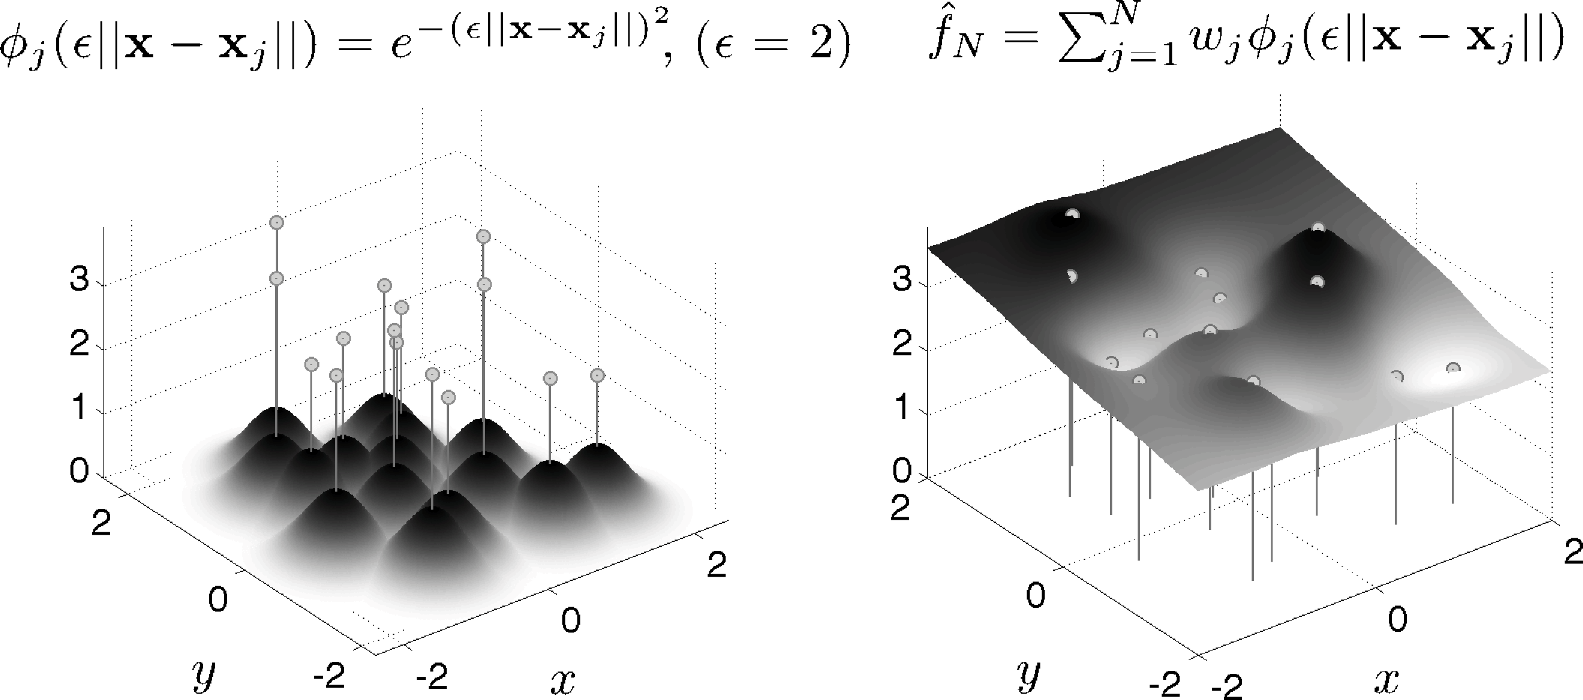
\includegraphics[scale=0.4]{figures/paper1/figures/trimmed_interpolate2D_ga__m_GRAY.pdf}
    \caption{RBF interpolation using 15 translates of the Gaussian RBF with $\epsilon=2$. One RBF is centered at each node in the domain. Linear
    combinations of these produce an interpolant over the domain passing through known function values. }
    \label{fig:rbfInterpolation}
\end{figure}

%To our knowledge, this paper presents the first implementation of RBF-FD 
Within this dissertation, we have developed the first implementation of RBF-FD
to span multiple CPUs. Each CPU has a corresponding GPU attached to it
in a one-to-one correspondence. We thus also introduced the first known 
implementation of accelerated RBF-FD on the GPU. \hl{continue with outline of chapters} 
We present our explicit and implicit solutions to PDEs with our multi-GPU RBF-FD implementation. 
%Within the scope of this paper we detail our method for spanning RBF-FD across multiple CPU/GPU processors and emphasize numerical validation of the implementation rather than optimization strategies. We will consider optimization in future work. The calculations are performed on Keeneland, a high performance computing installation supported by the National Science Foundation and located at Oak Ridge National Lab. Keeneland currently has 240 CPUs accompanied by 360 NVidia Fermi class GPUs with at least double that number expected by the end of 2012 \cite{Vetter2011}.

%The remainder of this paper is organized as follows:  Chapter~\ref{chap:rbffd} introduces RBF-FD via interpolation. Chapter~\ref{chap:gpu} details our parallelization strategies for the Keeneland system, including data partitions that are handled concurrently by different CPU processes and the data-parallel explicit time stepping scheme for the GPU. In Section~\ref{sec:validation}, our implementation is verified against well-known hyperbolic PDE test cases on the sphere, advection of a cosine bell and vortex wrap-up. Finally, performance benchmarks and results are presented in Section~\ref{sec:performance}, followed by conclusions and proposals for future optimization strategies in Section~\ref{sec:conclusion}.

\section{Cut from Paper1}



Sufficient understanding of RBF interpolation led to the development of the first global RBF method for PDEs in \cite{Kansa1990a}. Most popular among global methods is collocation, wherein RBF interpolation approximates the PDE solution by solving a large, dense linear system. 
In some cases RBF collocation demonstrates higher accuracy for the same number of nodes when compared to other state-of-the-art pseudospectral methods (e.g., \cite{Larsson2003} \cite{Flyer2007} \cite{Flyer2009b}). In \cite{Flyer2010}, spectral accuracy was demonstrated for hyperbolic PDEs even with local refinement of nodes in time.


Unfortunately---ill-conditioning aside---collocation methods are prohibitively expensive to solve when scaled to a large number of nodes. Assuming the collocation matrix does not change in time, global methods, with their dense systems, scale at $O(N^3)$ operations for initial preconditioning/preprocessing followed by $O(N^2)$ operations every time-step. This complexity is consistent with any collocation scheme. However, by introducing sparsity into the system (e.g., using compactly supported RBFs), the complexity is somewhat reduced.



General Purpose GPU (GPGPU) computing is one of today's hottest trends within scientific computing. 
The release of NVidia's CUDA at the end of 2006 marked both a 
redesign of GPU architecture, plus the addition of a new software layer that finally made GPGPU accessible to the general public. The CUDA API includes routines for memory control, interoperability with graphics contexts (i.e., 
OpenGL programs), and provides GPU implementation subsets of BLAS and FFTW libraries \cite{CudaGuide2011}. After the undeniable success of CUDA for C, new projects emerged to encourage GPU programming in languages like FORTRAN (see e.g., HMPP \cite{HMPP2009} and Portland Group Inc.'s CUDA-FORTRAN \cite{CudaFortran2009}). 

In early 2009, the Khronos Group--the group responsible for maintaining OpenGL--announced a new specification for a general 
parallel programming lanugage referred to as the Open Compute Language (OpenCL) \cite{OpenCL2009}. Similar in design to the CUDA language---in many ways it is a simple refactoring of the predecessor---the goal of OpenCL is to provide a mid-to-low level API and language to control any multi- or many-core processor in a uniform fashion. Today, OpenCL drivers exist for a variety of hardware including NVidia GPUs, AMD/ATI CPUs and GPUs, and Intel CPUs. 

This \textit{functional portability} is the cornerstone of the OpenCL language. However, functional portability does not imply performance portability. That is, OpenCL allows developers to write kernels capable of running on all types of target hardware, but optimizing kernels for one type of target (e.g., GPU) does not guarantee the kernel will run efficiently on another target (e.g., CPU).
% Already, today, CPUs are tending toward many core architectures. Simultaneously, the once specialized many-core GPUs now offer general purpose functionality. New architectures like the AMD Fusion \cite{AMDFusion} join CPU and GPU on the same chip proving that 
%, and It is easy to see that soon the CPU and GPU will meet somewhere in the middle as general purpose many-core architectures. OpenCL is an attempt to standardize programming before this intersection occurs. 
With CPUs tending toward many cores, and the once special purpose, many-core GPUs offering general purpose functionality, it is easy to see that soon the CPU and GPU will meet somewhere in the middle as general purpose many-core architectures. Already, ATI has introduced the Fusion APU (Accelerated Processing Unit) which couples an AMD CPU and ATI GPU within a single die. OpenCL is an attempt to standardize programming ahead of this intersection. 

%Home computers, smart-phones and other devices containing many- or multi-core compute units internally have driven the generalization of the accelerator language to provide a unified approach to targeting any available hardware. 

Petascale computing centers around the world are leveraging GPU accelerators to achieve peak performance. In fact, many of today's high performance computing installations boast significantly more GPU accelerators than CPU counterparts. The Keeneland project is one such example, currently with 240 CPUs accompanied by 360 NVidia Fermi class GPUs with at least double that number expected by the end of 2012 \cite{Vetter2011}. 

Such throughput oriented architectures require developers to decompose problems into thousands of independent parallel tasks in order to fully harness the capabilities of the hardware. To this end, a plethora of research has been dedicated to researching algorithms in all fields of computational science. Of interest to us are methods for atmospheric- and geo-sciences. 

%!TEX root = karen.tex


\chapter{The RBF-generated Finite Differences Method}

This chapter introduces our numerical method of choice, the Radial Basis Function-generated Finite Differences (RBF-FD). We start with a simple explanation of the method in terms of function expansion and interpolation, then provide examples operators used to calculate weights within this work. 

\section{Stencil-based Derivative Approximation}

The RBF-FD method approximates derivatives at a single node with a weighted combination of functions values at the node and its neighbors. 

Similar to standard Finite Differences, a stencil is generated connecting the center node and its nearest neighbors. In Figure~\ref{fig:stencil_example} we

\begin{figure}[htbp]
	\centering
	\begin{subfigure}[b]{0.40\textwidth}
		\centering
		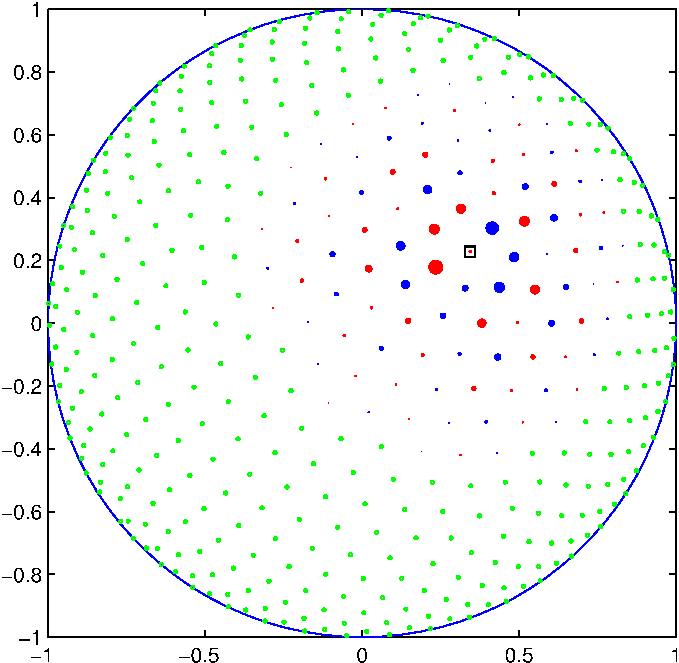
\includegraphics[width=1.0\textwidth]{figures/chapter1/RBFFD_single-eps-converted-to.pdf}
		\caption{A 75 node RBF-FD stencil with blue (negative) and red (positive) differentiation weights to approximate advective operator at the square.}
	\end{subfigure}
	\begin{subfigure}[b]{0.55\textwidth}
		\centering
		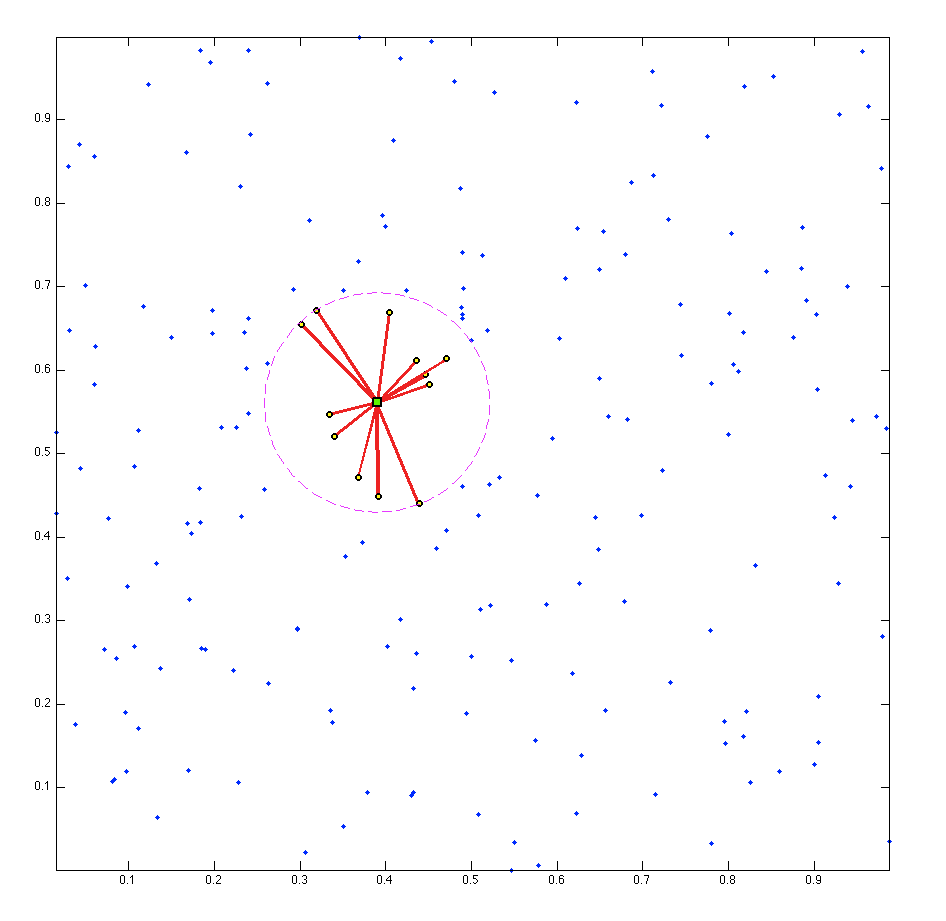
\includegraphics[width=1.0\textwidth]{figures/chapter1/preview_stencils_example.png}
		\caption{A 13 node RBF-FD stencil in a square domain of randomly distributed nodes. Stencil is centered at the green square.}
	\end{subfigure}
\end{figure}


\section{RBF-FD weights}
\label{sec:rbffd}

Given a set of function values, $\{u(\vx_j)\}_{j=1}^{N}$, on a set of $N$ nodes $\{\vx_j\}_{j=1}^{N}$, the operator $\diffop$ acting on $u(\vx)$ evaluated at 
$\vx_j$, %$u(\vx_j)$ 
is approximated by a weighted combination of function values, $\{u(\vx_i)\}_{i=1}^{n}$, in a small neighborhood of $\vx_j$, 
where $n\ll N$ defines the size of the stencil. 
%(added constant term to equation:)
\begin{align}
\diffop{u(\vx)}\mid_{\vx=\vx_j} &\approx \sum_{i=1}^{n} w_i u(\vx_i) + w_{n+1} p_0
\label{eq:derivFromFDWeights}
\end{align}
The RBF-FD weights, ${w_i}$, are found by enforcing that they are exact within the space spanned by the RBFs $\phi_i(\epsilon r) = \phi(\ep\vectornorm{\vx-\vx_{i}})$, centered at the nodes $\{\vx_i\}_{i=1}^{n}$, with 
$r=\vectornorm{\vx - \vx_i}$
being the distance between where the RBF is centered and where it is evaluated as measured in the standard Euclidean 2-norm. Various studies show  \cite{WrightFornberg06,FornbergDriscoll02,FornbergLehto11,FlyerLehto11} that better accuracy is achieved when the 
interpolant can exactly reproduce a constant, $p_0$.  
Assuming $p_0 = 1$, the constraint $\sum_{i=1}^{n}w_i=\diffop{1}|_{\vx=\vx_{j}}=0$ completes the system: 
%Address how the constraint is added. $w_{n+1}$ is mentioned without being defined.
%($\epsilon$ has been moved outside the norm on the RHS)
\begin{align}
\begin{pmatrix}
\phi(\epsilon\vectornorm{\vx_1-\vx_1}) & \phi(\epsilon\vectornorm{\vx_1-\vx_2} & \cdots & \phi(\epsilon\vectornorm{\vx_1-\vx_n}) & 1 \\
\phi(\epsilon\vectornorm{\vx_2-\vx_1}) & \phi(\epsilon\vectornorm{\vx_2-\vx_2} & \cdots &
\phi(\epsilon\vectornorm{\vx_2-\vx_n}) & 1\\
\vdots & \ddots & \ddots & \vdots & \vdots\\
\phi(\epsilon\vectornorm{\vx_n-\vx_1}) & \phi(\epsilon\vectornorm{\vx_n-\vx_2} & \cdots &
\phi(\epsilon\vectornorm{\vx_n-\vx_n}) & 1 \\
1 & 1 & \cdots & 1 & 0
\end{pmatrix}
\begin{bmatrix} w_1 \\ w_2 \\ \vdots \\ w_n  \\ w_{n+1}\end{bmatrix}
&=
\begin{bmatrix} \diffop{\phi(\ep\vectornorm{\vx-\vx_{1}})}|_{\vx=\vx_{j}} \\
                \diffop{\phi(\ep\vectornorm{\vx-\vx_{2}})}|_{\vx=\vx_{j}} \\ \vdots \\  \diffop{\phi(\ep\vectornorm{\vx-\vx_{n}})}|_{\vx=\vx_{j}}\\
                0
\end{bmatrix},
\label{eq:rbffd_weight_system}
\end{align}
where $w_{n+1}$ is ignored after the matrix in ({\ref{eq:rbffd_weight_system}}) is inverted.
This $n \times n$ system solve is repeated for each stencil center  $\vx_j$, $j=1...N$, to form the $N$ rows of the DM  with $n$ non-zeros $(n\ll N)$ per row.
As an example, if $\diffop$ is the identity operator, 
then the above procedure leads to RBF-FD interpolation. If $\diffop=\pd{}{x}$, one obtains the DM that approximates the first derivative in $x$. In the context of time-dependent PDEs,  the stencil weights remain constant for all time-steps when the nodes are stationary. Therefore, the calculation of the 
differentiation weights is performed once in a single preprocessing step of O$(n^3N)$ 
%floating point operations (FLOPs). 
FLOPs.
Improved efficiency is achieved
by processing multiple right hand sides in one pass, calculating the weights
corresponding to all required derivative quantities (i.e., $\pd{}{x}$, $\pd{}{y}$, $\Laplacian$, etc.).

%reply to the LSH question from the reviewer involving parallelization of the search process for each point, and the issue regarding embarrassingly parallel process. Also note: this is done only once so efficiency is not an issue, nor is parallelization.

For each of the $N$ small system solves of Equation~(\ref{eq:rbffd_weight_system}), the $n$ nearest neighbors to $\vx_j$ need to be located. This can be done efficiently using neighbor query algorithms or spatial partitioning data-structures such as Locality Sensitive Hashing (LSH) and $k$D-Tree. Different query algorithms often have a profound impact on the DM structure and memory access patterns. We choose a Raster ($ijk$) ordering LSH algorithm \cite{Bollig2011} leading to the matrix structure in Figures~\ref{fig:oneThreadPerStencil} and \ref{fig:oneWarpPerStencil}. While querying neighbors for each stencil is an embarrassingly parallel operation, the node sets used here are stationary and require stencil generation only once. Efficiency and parallelism for this task has little impact on the overall run-time of tests, which is dominated by the time-stepping. We preprocess node sets and generate stencils serially, then load stencils and nodes from disk at run-time. In contrast to the RBF-FD view of a static grid, Lagrangian/particle based PDE algorithms promote efficient parallel variants of LSH in order to accelerate querying neighbors at each time-step \cite{Pan2011, Goswami2010}. 


\section{Weight Operators}
Throughout the development of our parallel code we have verified code correctness through the solution of a variety of PDEs. Here we provide a list of operators we have tested and their corresponding equations for the RHS of Equation~\ref{eq:rbffd_weight_system} necessary to compute RBF-FD weights. 

The standard first derivatives $\pd{}{x}, \pd{}{y}, \pd{}{z}$:
\begin{itemize}
	\item $\pd{\phi}{x}  $
\end{itemize} 

where $\pd{\phi}{r}$ for the Gaussian RBFs is given by: 


\subsection{Laplacian ($\Laplacian$)}

2D: 

3D: 

\subsection{Laplace-Beltrami ($\LaplaceBeltrami$) on the Sphere}

The $\Laplacian$ operator can be represented in spherical polar coordinates for $\mathbb{R}^3$ as: 
\begin{align} 
\Laplacian = \underbrace{\frac{1}{r} \pd{}{r} \left( r^{2} \pd{}{r}  \right)}_{\mathsf{radial}} + \underbrace{\frac{1}{r^2} \Delta_{S}}_{\mathsf{angular}} , \label{eq:laplacian_in_spherical}
\end{align}
where $\LaplaceBeltrami$ is the Laplace-Beltrami operator---i.e., the Laplacian operator constrained to the surface of the sphere. This form nicely illustrates the separation of components into radial and angular terms. 

In the case of PDEs solved on the unit sphere, there is no radial term, so we have:
\begin{align}
\Laplacian  \equiv \LaplaceBeltrami.
\end{align}
Although this originated in the spherical coordinate system, \cite{WrightFlyerYuen10} introduced the following Laplaci-Beltrami operator for the surface of the sphere: 
\begin{align} 
\LaplaceBeltrami = \frac{1}{4} \left[ \left(4-r^2\right) \pdd{}{r} + \frac{4-3r^2}{r} \pd{}{r} \right],
\end{align} 
where $r$ is the Euclidean distance between nodes of an RBF-FD stencil and is independent of our choice of coordinate system. 

\subsection{Constrained Gradient ($P_{x} \cdot \grad$) on the Sphere}

Additionally following \cite{FlyerWright09, FlyerLehto11}, the gradient operator must also be constrained to the sphere with this projection matrix: 
%\frac{1}{||\mathbf{x}||}
\begin{align}
P = I - \mathbf{x} \mathbf{x}^T =  \begin{pmatrix} 
(1-x_1^2) & -x_1 x_2 & -x_1 x_3 \\
-x_1 x_2 & (1-x_2^2) & -x_2 x_3 \\ 
-x_1 x_3 & -x_2 x_3 & (1-x_3^2) 
\end{pmatrix} = \begin{pmatrix} P_{x_1} \\ P_{x_2} \\ P_{x_3} \end{pmatrix}
\label{eq:project_gradient}
\end{align}
where $\mathbf{x}$ is the unit normal at the stencil center. 


The direct method of computing RBF-FD weights for the projected gradient for $\mathbf{P} \cdot \nabla $ is presented in \cite{FlyerWright09}. When solving for the weights, we apply the projection on the right hand side of our small linear system. We let $\vx = \begin{pmatrix} x_1, x_2, x_3 \end{pmatrix} $ be the stencil center, and $\vx_k=\begin{pmatrix} x_{1,k}, x_{2,k}, x_{3,k}\end{pmatrix}$ indicate an RBF-FD stencil node. 

Using the chain rule, and assumption that 
$$r(\vx_k-\vx)=\vectornorm{\vx_k-\vx} = \sqrt{(x_{1,k}-x_1)^2 + (x_{2,k}-x_2)^2 + (x_{3,k}-x_3)^2},$$
 we obtain the unprojected gradient of $\phi$ as
$$\nabla \phi(r(\vx_k - \vx)) = \pd{r}{\vx} \pd{\phi(r(\vx_k - \vx))}{r} = - (\vx_k - \vx)\frac{1}{r(\vx_k - \vx)} \pd{\phi(r(\vx_k - \vx))}{r}$$. 

Applying the projection matrix gives 
\begin{align*}
\mathbf{P} \nabla \phi(r(\vx_k - \vx)) & = - (\mathbf{P} \cdot \vx_k - \mathbf{P}\cdot\vx)\frac{1}{r(\vx_k - \vx)} \pd{\phi(r(\vx_k - \vx))}{r} \\
& =  - (\mathbf{P}\cdot\vx_k - 0)\frac{1}{r(\vx_k - \vx)} \pd{\phi(r(\vx_k - \vx))}{r} \\
& = - (I-\vx\vx^T)(\vx_k
)\frac{1}{r(\vx_k - \vx)} \pd{\phi(r(\vx_k - \vx))}{r} \\
& = \begin{pmatrix} x \vx^T \vx_k - x_k \\ y \vx^T \vx_k -  y_k \\ z \vx^T \vx_k -z_k \end{pmatrix} \frac{1}{r(\vx_k - \vx)} \pd{\phi(r(\vx_k - \vx))}{r} 
 \end{align*}
Thus, when computing RBF-FD weights for the projected gradient we directly compute the weights using these RHS for the small stencil weight linear systems: 
\begin{align} 
P\pd{}{x_1} = ( x_1 \vx^T \vx_k - x_{1,k}) \frac{1}{r(\vx_k - \vx)} \pd{\phi(r(\vx_k - \vx))}{r} |_{\vx=\vx_j} \\
P\pd{}{x_2} = ( x_2 \vx^T \vx_k - x_{2,k}) \frac{1}{r(\vx_k - \vx)} \pd{\phi(r(\vx_k - \vx))}{r} |_{\vx=\vx_j} \\
P\pd{}{x_3} = ( x_3 \vx^T \vx_k - x_{3,k}) \frac{1}{r(\vx_k - \vx)} \pd{\phi(r(\vx_k - \vx))}{r} |_{\vx=\vx_j}
\end{align}



\section{Stabilization: Hyperviscosity}

For RBF-FD, differentiation matrices encode convective operators of the form 
\begin{equation}
D = \alpha \pd{}{\lambda} + \beta \pd{}{\theta} \label{eqconv}
\end{equation}
where $\alpha$ and $\beta$ are a function of the fluid velocity. The convective operator, discretized
through RBF-FD, has eigenvalues 
%given 
 in the right half-plane causing the method to be unstable~\cite{FornbergLehto11, FlyerLehto11}. 
%. 
%Shorter previous sentence. What diff operator is being discretized by DM?
Stabilization of the RBF-FD method is achieved through the application of a hyperviscosity filter 
to Equation~(\ref{eqconv}) \cite{FornbergLehto11}. By using Gaussian 
 RBFs, $\phi(r) = e^{-(\epsilon r)^2}$, the hyperviscosity (a high order Laplacian operator) simplifies to
\begin{equation}
\Delta^{k}\phi(r) = \epsilon^{2k} p_k(r) \phi(r)
\label{eqn:gaussian_hv}
\end{equation}
where $k$ is the order of the Laplacian and  $p_k(r)$ are multiples of generalized Laguerre polynomials that
are generated recursively (see \cite{FornbergLehto11}: Section 3.2). We assume a 2D  Laplacian operator 
when working on the surface of the sphere since a local stencil can be viewed as lying on a plane.
%Since the purpose of hyperviscosity is to suppress the highly oscillatory modes while leaving all the smooth ones intact, it suffices to ignore the local curvature of the sphere, and calculate $\Delta^{k}\phi(r)$ as if the RBF-FD stencil was located on a 2D flat plane.
%A 2D approximation for the hyperviscosity suffices because its only role is to suppress spurious unphysical modes. The scale of hyperviscosity, on the order of $10^{-30}$, makes this a completely harmless assumption even in the case when the stencil radius is large relative to the size of the sphere.

%I do not understand question 2.8

In the case of parabolic and hyperbolic PDEs, hyperviscosity is added as a filter to the right hand side of the evaluation. For example, at the continuous level, 
the equation solved takes the form
\begin{equation}
\pd{u}{t} = - D u + H u,
\label{eq:evaluation_with_hyperviscosity}
\end{equation}
%Address the issue of continuous versus discrete form. Use words operator and matrix properly. \authnote{Double check}
where $D$ is the PDE operator, and $H$ is the hyperviscosity filter operator.
Applying hyperviscosity shifts all the eigenvalues of D to the left half of the complex plane. 
This shift is controlled by $k$, the order of the Laplacian, and a scaling parameter $\gamma_c$, defined by
\begin{equation*}	
H = \gamma \Delta^{k} = \gamma_c N^{-k} \Delta^{k}.
\end{equation*}
Given a choice of $\epsilon$ (see Section~\ref{sec:numerical_validation}), it was found experimentally that $\gamma = \gamma_c N^{-k}$  provides stability and good accuracy for all values of $N$ considered here. It also ensures that the viscosity vanishes as $N\rightarrow\infty$ \cite{FlyerLehto11}.
In general, the larger the stencil size, the higher the order of the Laplacian.  This is attributed to the fact that, for convective operators, larger stencils treat a wider range of modes accurately. As a result, the hyperviscosity operator should preserve as much of that range as possible. The parameter $\gamma_c$ must also be chosen with care and its sign depends on $k$ (for $k$ even, $\gamma_c$ will be negative and for $k$ odd, it will be positive). If $\gamma_c$ is too large, the eigenvalues move outside the stability domain of our time-stepping scheme and/or eigenvalues corresponding to lower physical modes are not left intact, reducing the accuracy of our approximation. If $\gamma_c$ is too small, eigenvalues remain in the right half-plane \cite{FornbergLehto11,FlyerLehto11}.

\section{Fragments (integrate above)}

Global RBF collocation methods pose the problem of interpolating a multivariate function $f : \domain
    \rightarrow \R$ where $\domain \subset \R^m$. Given a set of sample values
    $\{f(x_j)\}_{j=1}^{N}$ on a discrete set of nodes $X = \{x_j\}_{j=1}^{N}
    \subset \domain$, an approximation $\hat{f}_N$ can be constructed through
    linear combinations of interpolation functions. Here, we choose univariate,
    radially symmetric functions based on Euclidean distance ($\vnorm{\cdot}$), and use
    translates $\phi(x-x_j)$ of a single continuous real
    valued function $\phi$ defined on $\R$ and centered at $x_j$:
         \begin{equation*} 
         \phi(x) := \varphi(\vnorm{x}).
         \end{equation*} 
    %with a continuous function $\varphi$ on $\R_0^{+}$. 
    Here, $\varphi$ is a
    Radial Basis Function and $\phi$ the
    associated kernel. For simplification $\phi_j(x)$ refers to a kernel centered at $x_j$; i.e., $\varphi(\vectornorm{x-x_j})$.

   The interpolant $\hat{f}_N(x)$ requires a linear combination of translates:  
        \begin{equation*}
      %  \hat{f}_N(x) = \sum_{j=1}^{N} c_j \varphi(\vnorm{x-x_j})
        \hat{f}_N(x) = \sum_{j=1}^{N} c_j \phi_j(x)
        \end{equation*}
    with real coefficients $\{c_j\}_{j=1}^{N}$. Assuming the interpolant passes through
    known values of $f$; i.e., 
        \begin{equation*} 
        \hat{f}_N(x_i) = f(x_i),\ \ \ \ \ 1 \leq i \leq N, 
        \end{equation*}
    allows one to solve for coefficients if the following linear system is uniquely
    solvable: 
        \begin{equation*} 
        %\sum_{j=1}^{N} c_j \varphi(\vnorm{x_i-x_j}) = f(x_i),\ \ \ \ \ 1
        \sum_{j=1}^{N} c_j \phi_j(x_i) = f(x_i),\ \ \ \ \ 1
        \leq i \leq N. 
        \end{equation*} 
    This is true if the $N \by N$ matrix $\Phi$ produced by the linear system
%        \begin{align} 
%          \begin{pmatrix}  
%            \varphi(\vnorm{x_1 - x_1}) & \varphi(\vnorm{x_1 - x_2}) & \cdots & \varphi(\vnorm{x_1 - x_N}) \\ 
%            \varphi(\vnorm{x_2 - x_1}) & \varphi(\vnorm{x_2 - x_2}) & \cdots & \varphi(\vnorm{x_2 - x_N}) \\ 
%            \vdots & \ddots & \ddots & \vdots \\
%            \varphi(\vnorm{x_N - x_1}) & \varphi(\vnorm{x_N - x_2}) & \cdots & \varphi(\vnorm{x_N - x_N})
%                \end{pmatrix} 
%                \begin{bmatrix} c_1 \\ c_2 \\ \vdots \\ c_N \end{bmatrix}
%               &=                \begin{bmatrix} f(x_1) \\ f(x_2) \\ \vdots \\ f(x_N) \end{bmatrix} \\
%                         \Phi \vec{c} &= \vec{f} 
%        \end{align} 
        \begin{align*} 
          \begin{pmatrix}  
            \phi_1(x_1) & \phi_2(x_1) & \cdots & \phi_N(x_1) \\ 
            \phi_1(x_2) & \phi_2(x_2) & \cdots & \phi_N(x_2) \\ 
            \vdots & \ddots & \ddots & \vdots \\
            \phi_1(x_N) & \phi_2(x_N) & \cdots & \phi_N(x_N)
                \end{pmatrix} 
                \begin{bmatrix} c_1 \\ c_2 \\ \vdots \\ c_N \end{bmatrix}
               &=                \begin{bmatrix} f(x_1) \\ f(x_2) \\ \vdots \\ f(x_N) \end{bmatrix} \\
                         \Phi \vec{c} &= \vec{f} 
        \end{align*} 
is nonsingular.

 When choosing an appropriate basis function for interpolation, a
    subset of RBFs have been shown to produce symmetric positive definite
    $\Phi$, while others are only conditionally positive definite (for more details see
    \cite{Fasshauer2007}).  With
    the latter set, additional polynomial terms are added to constrain the
    system and enforce positive definiteness, resulting in this expanded system of equations: 
        \begin{align} 
       % \sum_{j=1}^{N} c_j \varphi(\vnorm{x_i-x_j}) + \sum_{k=1}^{t}d_k p_k(x_i) &= f(x_i),\ \ \ \ \ 1
        \sum_{j=1}^{N} c_j \phi_j(x_i) + \sum_{k=1}^{M}d_k p_k(x_i) &= f(x_i),\ \ \ \ \ 1
        \leq i \leq N, \nonumber \\ 
        \sum_{j=1}^{N} c_j p_k(x_j) &=  0,\ \ \ \ \ \ \ \ \ \ 1 \leq k \leq M. \nonumber \\
          \begin{pmatrix} \Phi & P \\ P^T & 0 \end{pmatrix} \begin{bmatrix} c \\ d \end{bmatrix} &= \begin{bmatrix} \vec{f} \\ 0 \end{bmatrix}
	\label{eq:additional_constraints}
        \end{align} 
        where $\{p_k\}_{k=1}^{M}$ is a basis for $\Pi_{p}^{m} $ (the set of polynomials in $m$ variables of degree $\leq p$) and 
       \begin{equation*}
       M = {{p+m}\choose{m}}       .
       \end{equation*} 
      %\authnote{Add table? or cut:} Table~\ref{tbl:rbfoptions} provides example RBF functions and notes their (conditionally) positive definiteness. 


Given the coefficients $\vec{c}$, the function value at a test point $x$ is interpolated by
\begin{align}	 
	\hat{f}_N(x) &= \sum_{j=1}^{N}c_j \Phi_j(x) + \sum_{l=1}^{M}d_l P_l(x)  \nonumber \\
	&=  \left[\begin{array}{cc}
        \Phi & \PP
	\end{array} \right] 
	 \begin{bmatrix}	c \\
					d
		 \end{bmatrix} \nonumber \\
						 &= \vec{\Phi}_x^T \vec{c} \nonumber \\
						 &= \vec{\Phi}_x^T \Phi^{-1}\vec{f}	
						 \label{eq:rbf_interpolate_pt}
\end{align}
where $\vec{c}$ is substituted by the solution to Equation~\ref{eq:additional_constraints}. In Equation~\ref{eq:rbf_interpolate_pt} the term $\Phi_{x}^T\Phi^{-1}$, dependent only on node positions, can be evaluated prior to knowing $f$. 

For the RBF-FD method, derivatives of $u(x)$ are weighted combinations of a small neighborhood of $N_s$ nodes (i.e., a stencil with $N_s \ll N$):
 %derivative of u (i.e., $\diffop{u}$) at the stencil center ($x_1$) as a weighted combination of neighbors (like typical Finite Differencing): 
        \begin{align} 
        \diffop{u(x_1)} &\approx \sum_{j=1}^{N_s} c_j u(x_j) \nonumber 
        \label{eq:derivFromFDWeights}
        \end{align}
where $\diffop{u}$ denotes a linear differential quantity over $u$ (e.g., $\diffop{u} = \d{u}{x}$). Here, ${c_j}$ are unknown, and obtained by enforcing the reconstruction:
	\begin{align}
	        \diffop{\phi_j(x_1)} = \sum_{i=1}^{N_s} c_i \phi_j(x_i) \ \ \ \ \ \ \textrm{for }j=1,2,...,N_s \nonumber 
	\end{align}
with $\diffop{\phi}_j$ provided by analytically applying the differential operator to the kernel function.
This is equivalent to: 
	\begin{align}        
          \begin{pmatrix}  
            \phi_1(x_1) & \phi_1(x_2) & \cdots & \phi_1(x_{N_s}) \\ 
            \phi_2(x_1) & \phi_2(x_2) & \cdots & \phi_2(x_{N_s}) \\ 
            \vdots & \ddots & \ddots & \vdots \\
            \phi_{N_s}(x_1) & \phi_{N_s}(x_2) & \cdots & \phi_{N_s}(x_{N_s})
                \end{pmatrix} 
                \begin{bmatrix} c_1 \\ c_2 \\ \vdots \\ c_N \end{bmatrix}
               &=                \begin{bmatrix} \diffop{\phi_1}(x_1) \\  \diffop{\phi_2}(x_1) \\ \vdots \\  \diffop{\phi_{N_s}}(x_1) 
               \end{bmatrix} \\
                         \Phi_{s} \vec{c} &= \vec{\Phi_{\diffop{}_s}}.% (x_1)
                         \label{eqn:rbffd_simplified}
                         % \Phi_{i,j} \vec{c} &= \vec{\diffop{\phi_j}} 
        \end{align} 
Solving Equation~\ref{eqn:rbffd_simplified} for stencils weights, $\vec{c}$, and substituting into Equation~\ref{eq:derivFromFDWeights} reveals the similarity between RBF-FD and the general problem of RBF interpolation (see Equation~\ref{eq:rbf_interpolate_pt} and discussion): 
        \begin{align*} 
        \diffop{u(x_1)} &\approx (\Phi^{-1}_s \vec{\Phi}_{\diffop{}_s})^T \vec{u} \\
        &\approx \vec{\Phi}_{\diffop{}_s}^T \Phi^{-T}_s \vec{u}
        \label{eq:rbffd_approx_derivs}
        \end{align*}
        
	
Again, based on the choice of RBF, positive definiteness of the system is ensured by adding the same constraints as Equation~\ref{eq:additional_constraints}, but note differential quantities for $\vec{\PP}$ on the right hand side: 
	\begin{align}
		\begin{pmatrix}
		\Phi_s & \PP \\
		\PP^T & 0
		\end{pmatrix} \begin{bmatrix}
							c \\ 
							d
							\end{bmatrix}
				 &= \begin{bmatrix}
							\vec{\Phi}_{\diffop{}_s} \\
							\vec{\PP}_{\diffop{}}
							 \end{bmatrix}.
	\end{align}
	%\authnote{must have things mixed up in my head. Cannot justify the reason to have $\PP_{\diffop{}}$ and not $0$. Perhaps because I dont fully understand the cardinal point derivation of RBFFD.}
Equation~\ref{eq:rbffd_approx_derivs} is strictly for the stencil centered at node $x_1$. To obtain weights for all stencils in the domain, a total of $N$ such systems must be solved. %Following the discussion of Equation~\ref{eq:rbf_interpolate_pt}, stencils weights are computed given only node positions. 


Stabilization of the RBF-FD method is achieved through the application of a hyperviscosity filter \cite{Fornberg2011b}. By assuming the use of Gaussian RBFs, $\phi(r) = e^{-(\epsilon r)^2}$, the hyperviscosity operator simplifies to
\begin{equation}
\Delta^{k}\phi(r) = \epsilon^{2k} p_k(r) \phi(r).
\label{eqn:gaussian_hv}
\end{equation}
The multiples of generalized Laguerre polynomials, $p_k(r)$, are obtained through the following recursive relation:
\begin{align*}
\begin{cases} 
p_0(r) &=1, \\
p_1(r) &= 4(\epsilon r)^2 - 2d, \\
p_k(r) &= 4((\epsilon r)^2 - 2(k-1) - \frac{d}{2})  p_{k-1}(r) - 8(k-1)(2(k-1) - 2 + d) p_{k-2}(r), \ \ \ \ k = 2, 3, ...
\end{cases}
\end{align*}
where $d$ is the dimension of the problem. We assume $d=2$ below when working on the surface of the sphere.

\chapter{Tabular Data and Tables}

Most graduate students will come to a place in their career where they
must create a table of some kind.  Many simple layouts are a breeze
with \LaTeX.  Here's a brief example:

\begin{quote}
\begin{tabular}{ r r || c | l }
  1  & a      & $3^1$                      &     3 \\
  2  & abb    & $3\times 3^2$              &    27 \\ \hline
  33 & abbccc & $3^3 \times 3^3 \times 3^3$ & 19683 \\
\end{tabular}
\hskip12pt and the source text that created it:
\begin{verbatim}
\begin{tabular}{ r r || c | l }
  1  & a      & $3^1$                       &     3 \\
  2  & abb    & $3\times 3^2$               &    27 \\ \hline
  33 & abbccc & $3^3 \times 3^3 \times 3^3$ & 19683 \\
\end{tabular}
\end{verbatim}
\end{quote}

When the \lit{tabular} environment begins, the next required parameter
specifies the layout of the table.  In this case, the table layout
specifies two right-justified columns (\lit{r r}), a double-vertical
separator (\lit{||}), a centered column (\lit{c}), a single-vertical
separator (\lit{|}), and a left-justified column (\lit{l}).  The next
rows provide the data for the table, with columns separated by the
ampersand (\verb|&|) character.  The end of the row is indicated by
the double backslash (\verb|\\|).  As you can see, the columns may
contain text, numeric data, and even some math.  A horizontal line may
be drawn between rows using the \verb|\hline| command.

For many people, this may be all the information on tables that's
required (for now, anyway).  But at some point, you may need even more
options to create just the right layout.  A quick web search for
\lit{latex table} will turn up a wealth of usable information,
samples, examples, and tutorials.

The \lit{tabular} environment provides the layout mechanism for
placing text and data into row and column form.  But it's the
\lit{table} environment that allows you to automatically number your
table and to add a heading (caption).  The \lit{table} environment
works just like the \lit{figure} environment as far as floating
placement is concerned.  However, the FSU thesis guidelines state that
table captions should appear \emph{before} the table, while
\lit{figure} captions appear \emph{after} the figure.  The text in
Figure~\ref{sonnet-text} generates Table~\ref{sonnets} as an example.
(And I used \verb|Table~\ref{sonnets}| in the previous sentence to
retrieve the table number.)  This demonstrates how one can create
paragraphs of text as part of a table by using the \verb|p{5cm}|
format specifier.  Additional space was inserted after each row by
adding a dimension to the linebreak specification, i.e., \verb|\\[5pt]|.

However, just because you put some text or data into a multi-column
form, it doesn't necessarily mean that it's a table as far as your
thesis or dissertation is concerned.  If the tabular-form data is part
of your text and flows in the order of your presentation, it may not
be necessary to set it off as a table.  The layout example at the
beginning of this chapter is an example of tabular data which is not
set off as a table.

Other than the unfortunately confusing similarity in their names, the
\lit{tabular} environment and the \lit{table} environment have
independent functionality: while the \lit{tabular} environment is
often used inside the \lit{table} environment, either environment can
be used without the other.  And while we're at it, figures don't
necessarily need to contain graphics.  Figure~\ref{sonnet-text} is an
example of a figure which contains ordinary text, but the text has
been wrapped within a \lit{figure} environment so that it can be
allowed to float outside the main flow of text.

If you have a particularly wide table, you may want to turn the table
sideways on the page.  To do this, you should place a
\verb|\usepackage{rotating}| in the document preamble.  When it is
time to insert the rotated table, type \verb|\begin{sidewaystable}|
instead of \verb|\begin{table}|.  This also works for figures, by the
way, so instead of \verb|\begin{figure}|, you may use
\verb|\begin{sidewaysfigure}| for diagrams and images that you want
rotated.  Sideways figures and tables will always be floated to their
own page.

\begin{figure}
% Centering doesn't work around a verbatim environment (it takes up the
% entire line-width), so we fake it by prefixing spaces to each line.
\begin{verbatim}
    \begin{table}
    \caption{Shakespeare Sonnets, First Lines, IIX --- XII}
    \label{sonnets}
    \begin{center}
      \begin{tabular}{r p{5cm} }
        8 & Music to hear, why hear'st thou music sadly? \\[5pt]
        9 & Is it for fear to wet a widow's eye \\[5pt]
       10 & For shame deny that thou bear'st love to any \\[5pt]  
       11 & As fast as thou shalt wane, so fast thou grow'st \\[5pt]
       12 & When I do count the clock that tells the time \\
      \end{tabular}
    \end{center}
    \end{table}
\end{verbatim}
\caption{\LaTeX{} source that generates Table~\ref{sonnets} on 
page~\pageref{sonnets}.}
\label{sonnet-text}
\end{figure}

\begin{table}
\caption{Shakespeare Sonnets, First Lines, IIX --- XII}
\label{sonnets}
\begin{center}
\begin{tabular}{r p{5cm} }
  8 & Music to hear, why hear'st thou music sadly? \\[5pt]
  9 & Is it for fear to wet a widow's eye \\[5pt]
 10 & For shame deny that thou bear'st love to any \\[5pt]  
 11 & As fast as thou shalt wane, so fast thou grow'st \\[5pt]
 12 & When I do count the clock that tells the time \\
\end{tabular}
\end{center}
\end{table}
 
%!TEX root = karen.tex

\chapter{Numerical Validation} 

\label{sec:validation}

\section{Stencil Generation} 
\subsection{kD-Tree vs LSH} 
\section{Choosing $\epsilon$}
Present our attemps to get the right support parameter


\section{Parabolic} 

Include figure tracking max temperature and min temperature. If we have zero flux conditions then they should average out. If we have Dirichlet BCs the temperature will converge to 0. 



\section{Hyperbolic} 

Here, we present the first results in the literature for parallelizing RBF-FDs on multi-CPU and multi-GPU architectures for solving PDEs. 
 To verify our multi-CPU, single GPU and multi-GPU implementations, two hyperbolic PDEs on the surface of the sphere are tested: 1) vortex roll-up \cite{NairTransport05, NairJablonowski08} and 2) solid body rotation \cite{JakobChien1995}. These tests were chosen since they are not only standard in the numerical literature, but also
for the development of RBFs in solving PDEs on the sphere \cite{FlyerWright07, Fornberg2008, FlyerLehto10, Fornberg2011a}. Although any `approximately evenly' distributed nodes on the sphere would suffice for our purposes, maximum determinant (MD) node distributions on the sphere are used (see \cite{Sloan2003} for details) in order to be consistent with previously published results (see e.g., \cite{FlyerWright07} and \cite{FornbergLehto11}). Node sets from 1024 to 27,556 are considered with stencil sizes ranging from 17 to 101.

All results in this section are produced by the single-GPU implementation. Multi-CPU and multi-GPU implementations are verified to produce these same results. Synchronization of the solution at each time-step and the use of double precision on both the CPU and GPU ensure consistent results regardless of the number and/or choice of CPU vs GPU. Eigenvalues are computed on the CPU by the Armadillo library \cite{armadillo2010}.

\subsection{Vortex Rollup}
\label{sec:numerical_validation}
The first test case demonstrates vortex roll-up of a fluid on the surface of a unit sphere. An angular velocity field causes the initial condition to spin into two diametrically opposed but stationary vortices.

The governing PDE in latitude-longitude coordinates, $(\theta,\lambda)$, is
\begin{equation}
\pd{h}{t} + \frac{u}{\cos \theta} \pd{h}{\lambda} = 0
\label{eq:vortex}
\end{equation}
where the velocity field, $u$, only depends on latitude and is given by
\begin{equation*}
u  = \omega(\theta) \cos \theta.
\end{equation*}
Note that the $\cos \theta$ in $u$ and $1/\cos{\theta}$ in (\ref{eq:vortex}) cancel in the analytic formulation, so the discrete operator approximates $\omega(\theta) \pd{}{\lambda}$. 

Here, $\omega(\theta)$ is the angular velocity component given by
\begin{equation*}
\omega(\theta) =
\begin{cases}
\frac{3\sqrt{3}}{2 \rho(\theta)} \mathrm{sech}^{2}(\rho(\theta)) \mathrm{tanh}(\rho(\theta)) & \rho(\theta) \neq 0 \\
0 & \rho(\theta) = 0
\end{cases}
\end{equation*}
where $\rho(\theta) = \rho_0 \cos \theta$ is the radial distance of the vortex with $\rho_0=3$. The exact solution to (\ref{eq:vortex}) at non-dimensional time $t$ is
\begin{equation*}
h(\lambda, \theta, t) = 1 - \mathrm{tanh}\left( \frac{\rho(\theta)}{\gamma} \sin(\lambda - \omega(\theta) t) \right),
\end{equation*}
where $\gamma$ defines the width of the frontal zone.

From a method of lines approach, the discretized version of (\ref{eq:vortex}) is
\begin{equation}
%\pd{\mathbf{h}}{t} = - \text{diag}(\omega(\theta)) D_\lambda \mathbf{h}.
\d{\mathbf{h}}{t} = - \text{diag}(\omega(\theta)) D_\lambda \mathbf{h}.
\label{eq:vortex_matrix_form}
\end{equation}
where $D_\lambda$ is the DM containing the RBF-FD weights that approximate $\pd{}{\lambda}$ at each node on the sphere.

For stability, hyperviscosity is added to the right hand side of (\ref{eq:vortex_matrix_form}) in the form given in (\ref{eq:evaluation_with_hyperviscosity}). The scaling parameter $\gamma_c$ and the order of hyperviscosity $k$ are given in
Table~\ref{tbl:vortex_hv_params}. The goal when choosing $k$ is to damp the higher spurious eigenmodes of $\text{diag}(\omega(\theta)) D_\lambda$ while leaving the lower physical modes that can be resolved by the stencil intact. In this process, the eigenvalues will be pushed into the left half of the complex plane. Then, $\gamma_c$ is used to condense the eigenvalues as near to the imaginary axis as possible. Figure \ref{fig:vortex_eigs_hv} shows the effect of hyperviscosity on the eigenvalues of the DM, $-diag(\omega(\theta)) D_\lambda$, in (\ref{eq:vortex_matrix_form}). 

In order to scale to large node sets, the RBF shape parameter, $\epsilon$, is chosen such that the mean condition number of the local RBF interpolation matrices $\bar{\kappa}_A = \frac{1}{N}\sum_{j=1}^N (\kappa_A)_j$ is kept constant as $N$ increases ($(\kappa_A)_j$ is the condition number of the interpolation matrix in (\ref{syst}), representing the $j^{th}$ stencil). For a constant mean condition number, $\epsilon$ varies linearly with $\sqrt{N}$ (see \cite{FlyerLehto11} Figure 4a and b). This is not surprising since the condition number strongly depends on the quantity $\epsilon r$, where $r\thicksim1/\sqrt{N}$ on the sphere. Thus, to obtain a constant condition number, we let $\epsilon (N) = c_1 \sqrt{N} - c_2$, where $c_1$ and $c_2$ are constants based on \cite{FlyerLehto11}.

\begin{table}[t]
\caption{Values for hyperviscosity and the RBF shape parameter $\epsilon$ for vortex roll-up test.}
\begin{center}
\begin{tabular}{|c|c|c|c|c|c|}
\hline		     & \multicolumn{2}{c|}{$\epsilon = c_1 \sqrt{N} - c_2$} & \multicolumn{2}{c|}{$H = -\gamma_{c} N^{-k} \Delta^{k}$ } \\ \hline
Stencil Size ($n$) & $c_{1}$ & $c_{2}$ & $k$ & $\gamma_c$ \\ \hline
17 & 0.026 & 0.08 & 2 & $8$ \\
31 & 0.035 & 0.1  & 4 & $800$ \\
50 & 0.044 & 0.14 & 4 & $145$ \\
101 & 0.058 & 0.16 & 4 & $40$ \\ \hline
\end{tabular}
\end{center}
\label{tbl:vortex_hv_params}
\end{table}



\begin{figure}[htb]
\begin{center}
\begin{subfigure}[b]{0.45\textwidth}
	\centering
	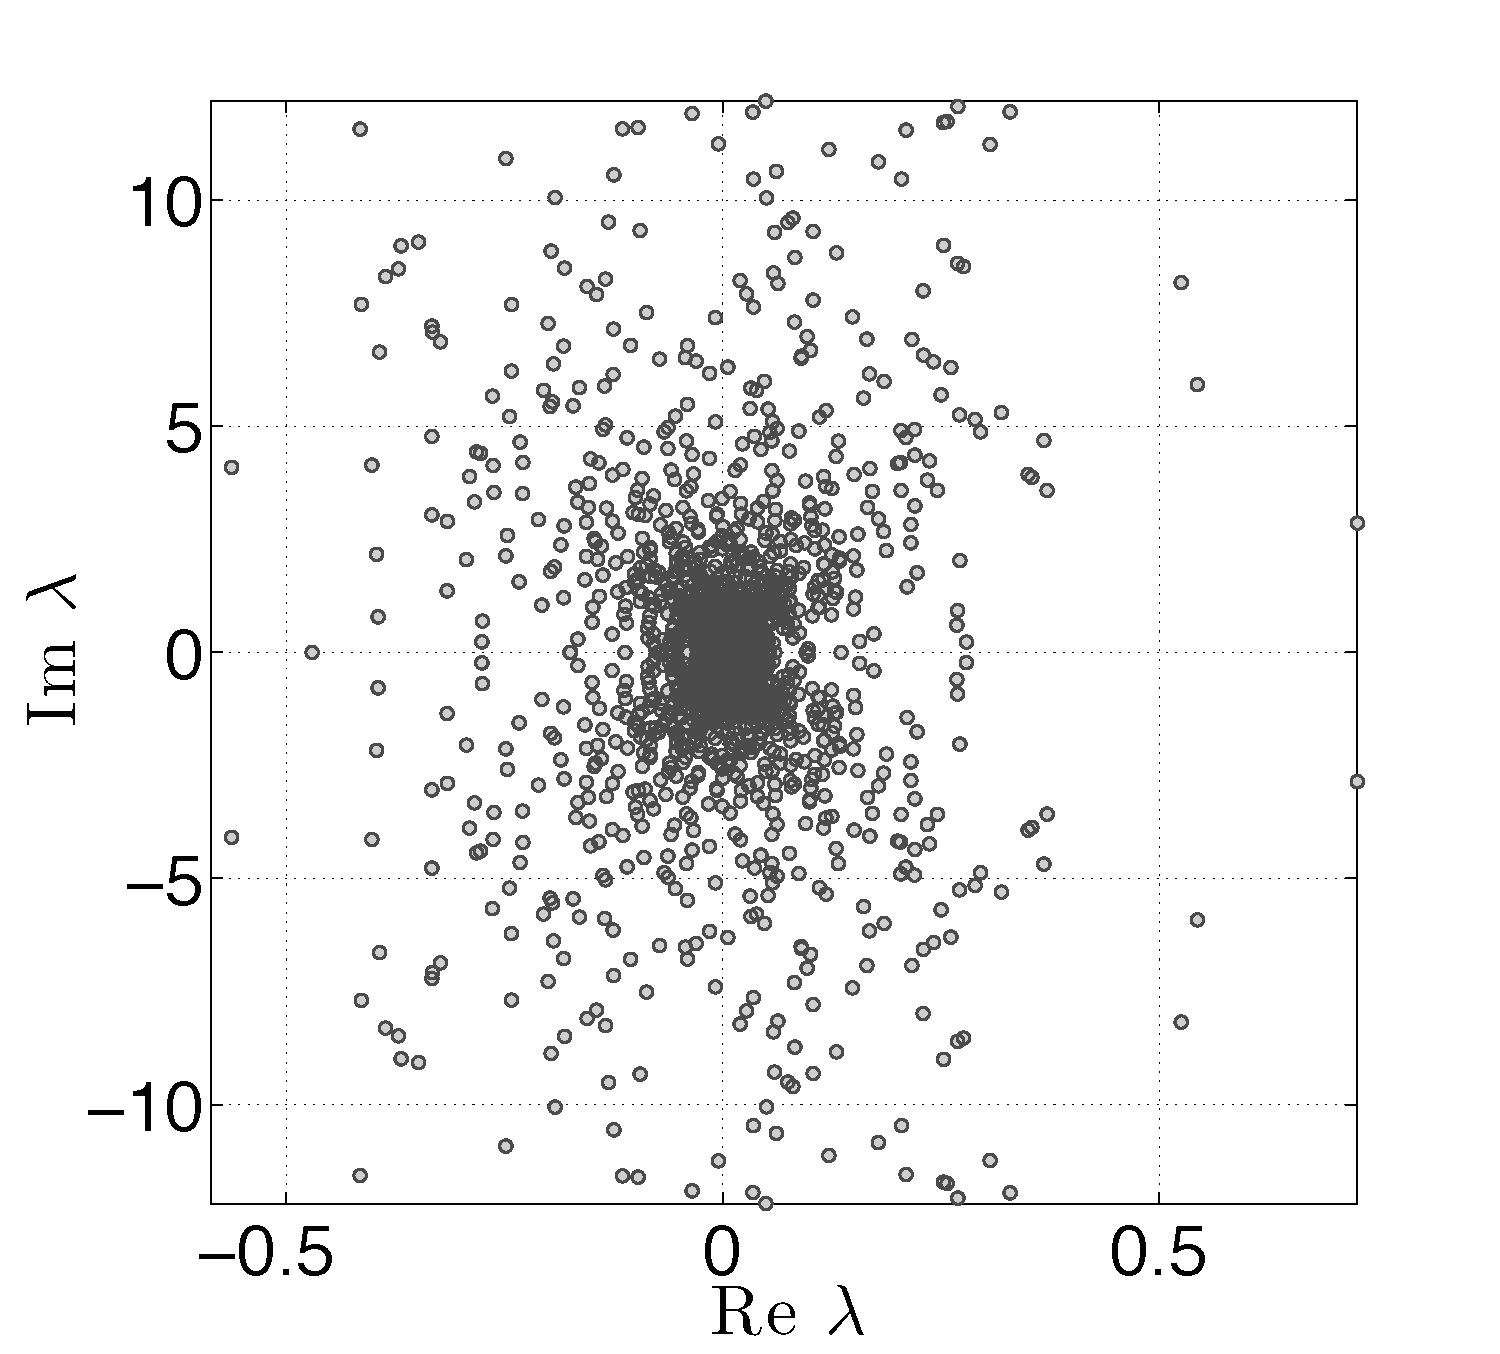
\includegraphics[width=1.0\textwidth]{figures/paper1/figures/vortex_rollup/eigs_N4096_n101_noHV.pdf}
	\caption{No Hypervsiscosity}
	\label{fig:vortex_eigs_nohv}
\end{subfigure}
\begin{subfigure}[b]{0.45\textwidth}
	\centering
	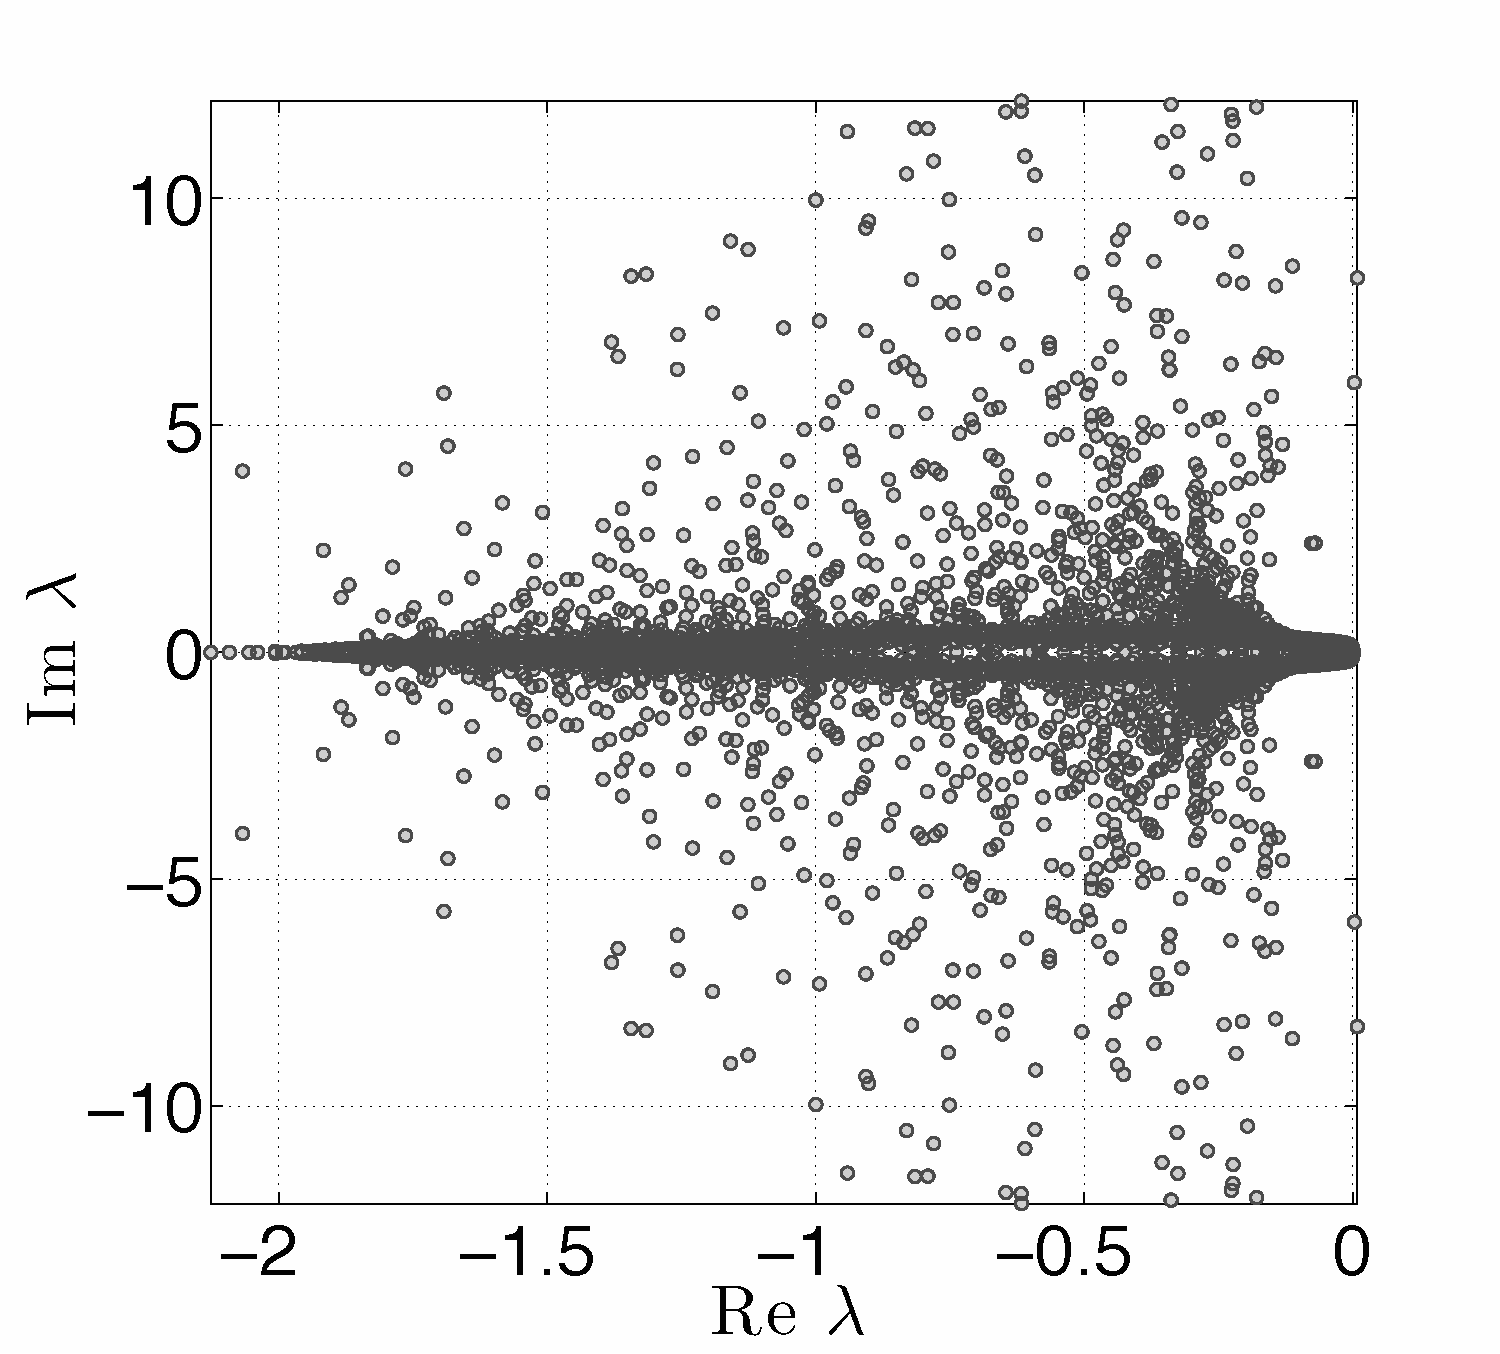
\includegraphics[width=1.0\textwidth]{figures/paper1/figures/vortex_rollup/eigs_N4096_n101_HV_k4_gamma40.pdf}
	\caption{With Hyperviscosity}
	\label{fig:vortex_eigs_hv}
\end{subfigure}
\caption{Eigenvalues of $\text{diag}(\omega(\theta)) D_\lambda$ for the vortex roll-up test case for $N=4096$ nodes, stencil size $n=101$ and $\epsilon = 3.5$. Left: no hyperviscosity. Right: hyperviscosity enabled with $k=4$ and $\gamma_c = 40$. }
\label{fig:eig_vortex}
\end{center}
\end{figure}

\begin{figure}[htbp]
\begin{center}
\begin{subfigure}[b]{0.45\textwidth}
	\centering
	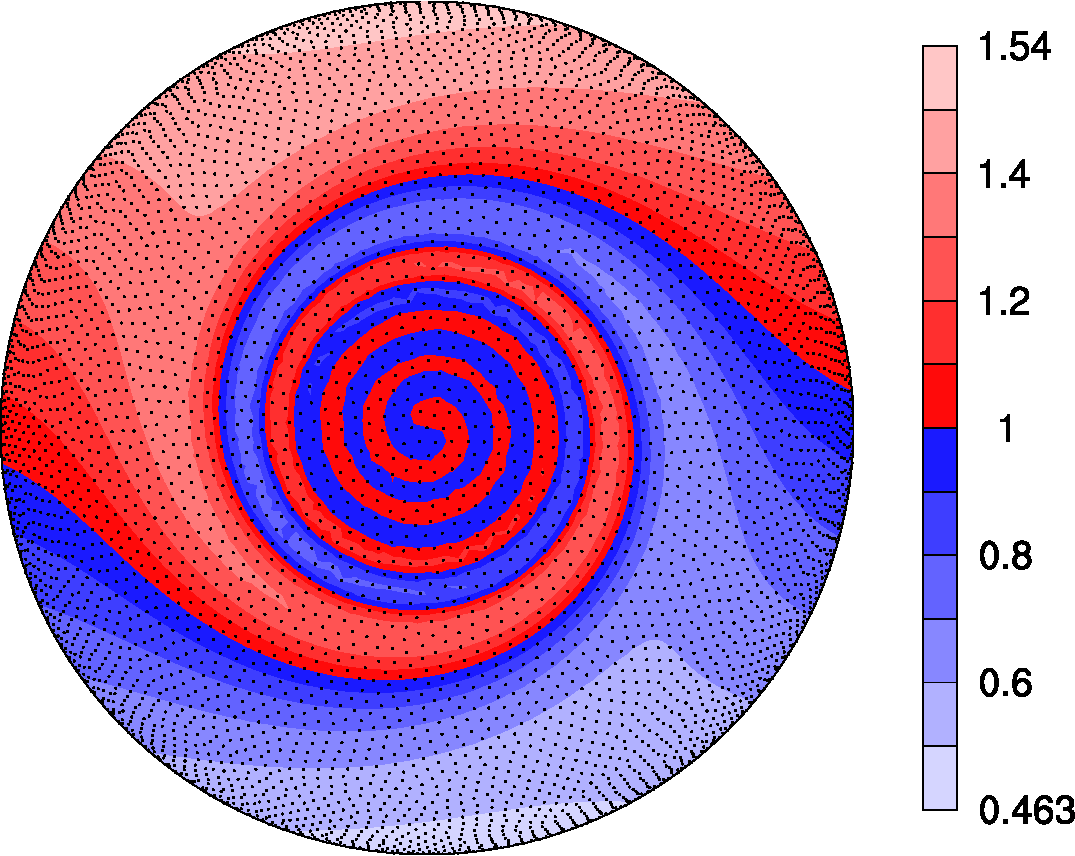
\includegraphics[width=1.0\textwidth]{figures/paper1/figures/vortex_rollup/vortexComputedSolution-eps-converted-to.pdf}
	\caption{Computed Solution}
	\label{fig:vortex_approx}
\end{subfigure} 
\begin{subfigure}[b]{0.45\textwidth}
	\centering
	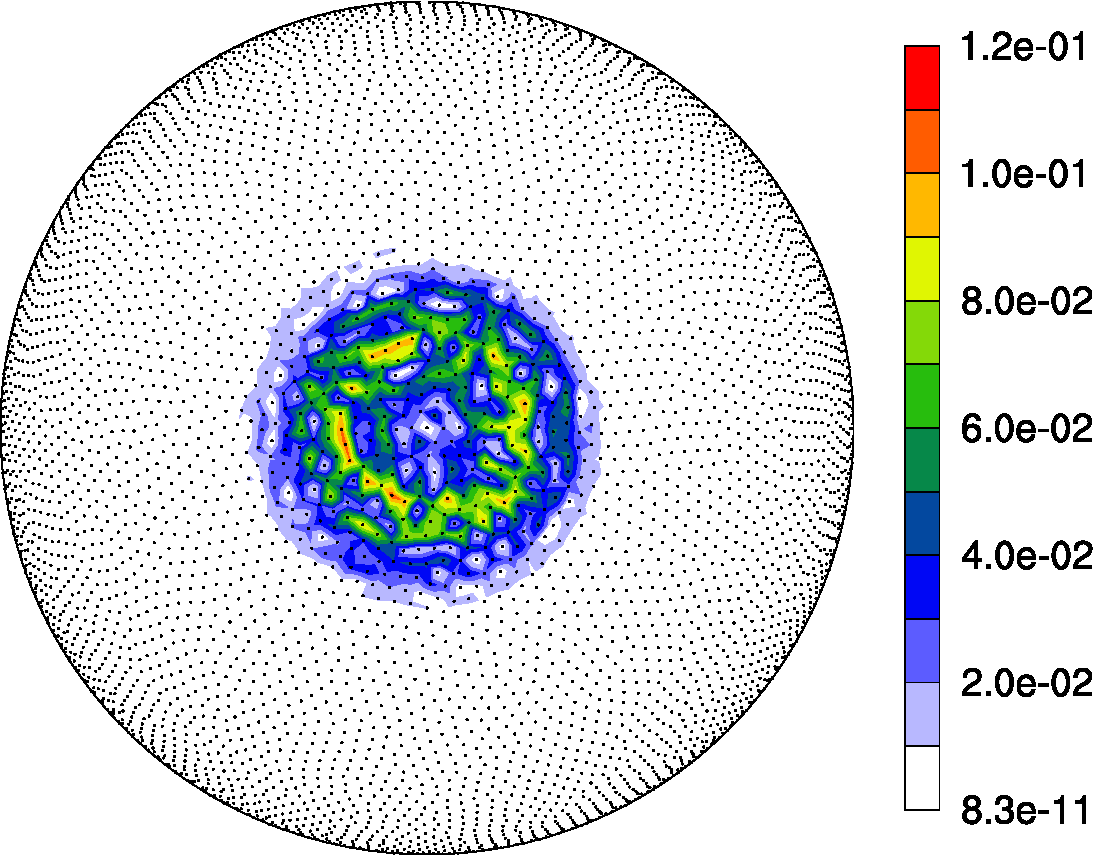
\includegraphics[width=1.0\textwidth]{figures/paper1/figures/vortex_rollup/vortexRelativeError-eps-converted-to.pdf}
	\caption{Relative Absolute Error}
	\label{fig:vortex_relerr}
\end{subfigure}
\caption{Vortex roll-up solution at time $t=10$ using RBF-FD with $N=10,201$ and $n=50$ point stencil. Normalized $\ell_2$ error of solution at $t=10$ is $1.25(10^{-2})$ }
\label{fig:vortex_t10}
\end{center}
\end{figure}

Figure~\ref{fig:vortex_t10} shows the solution to Equation~(\ref{eq:vortex}) at $t = 10$, on $N=10201$ nodes, with stencil size $n=50$. This resolution is sufficient to properly capture the vortices at $t=10$, but lower resolutions would suffer approximation errors associated with insufficient grid resolution. 
For this reason, the solution at $t=3$ is considered in the normalized $\ell_2$ error convergence study presented in Figure~\ref{fig:conv_plot_vortex_hv}. The time step $\Delta t = 0.05$ for all resolutions.

\begin{figure}[htbp!]
\begin{center}
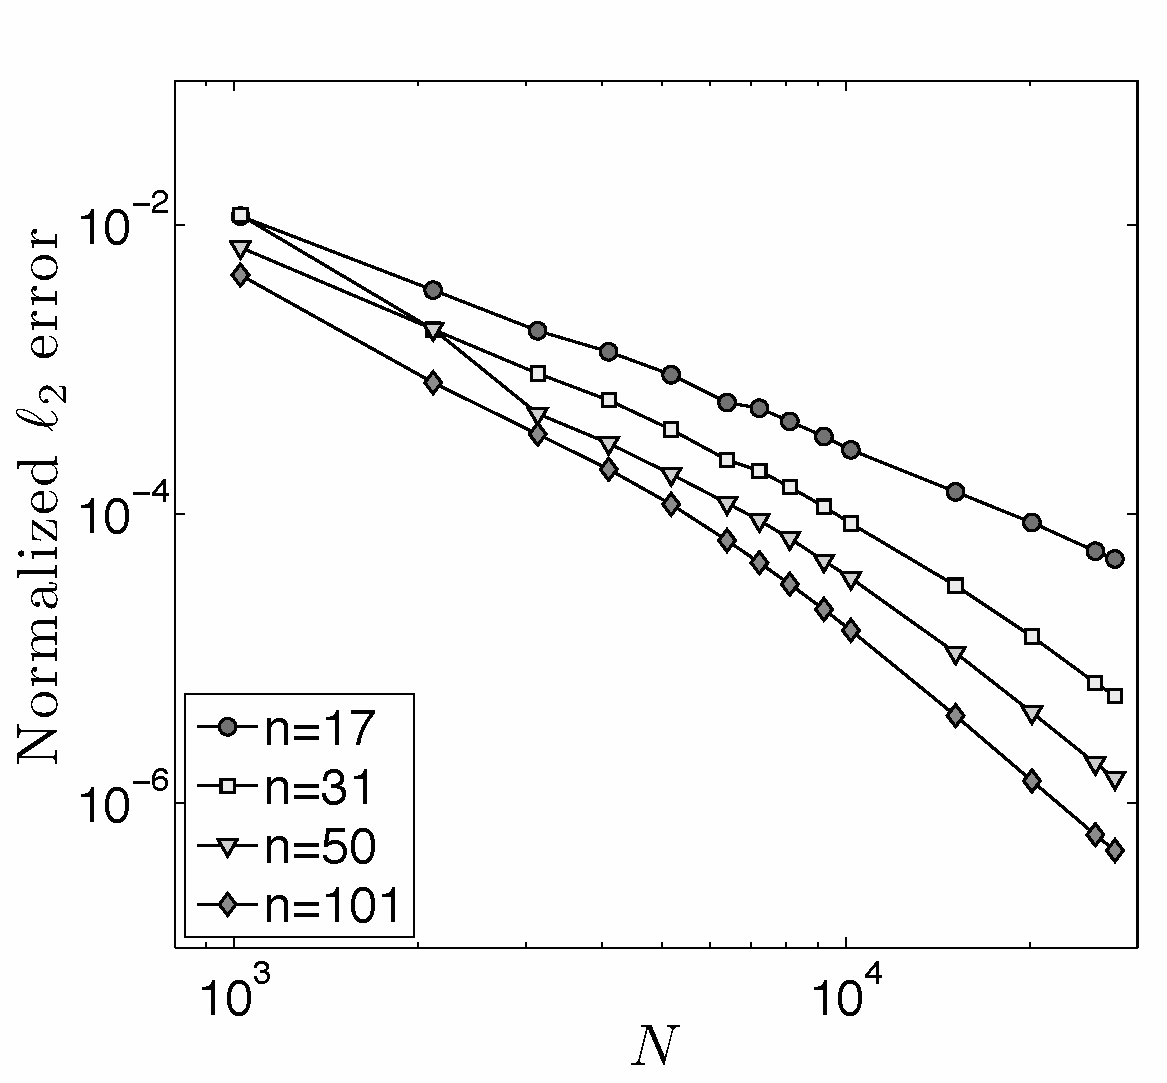
\includegraphics[width=3in] {figures/paper1/figures/vortex_rollup/convergence_plot_hv.pdf}
\caption{Convergence plot for vortex roll-up at $t=3$. }
\label{fig:conv_plot_vortex_hv}
\end{center}
\end{figure}

\subsection{Solid body rotation}

The second test case simulates the advection of a cosine bell over the surface of a unit sphere at an angle $\alpha$ relative to the pole of a standard latitude-longitude grid. The governing PDE is
\begin{equation}
\pd{h}{t} + \frac{u}{\cos \theta} \pd{h}{\lambda} + v \pd{h}{\theta} = 0, \label{eq:cosine_bell}
\end{equation}
with velocity field,
\begin{equation*}
%\begin{cases}
%u =  \cos \theta \cos \alpha + \sin \theta \cos \lambda \sin \alpha,  & \\
%v =  -\sin \lambda \sin \alpha &.
%\end{cases}
\begin{cases}
u =  u_0 (\cos \theta \cos \alpha + \sin \theta \cos \lambda \sin \alpha),  & \\
v =  -u_0(\sin \lambda \sin \alpha) &.
\end{cases}
\end{equation*}
inclined at an angle $\alpha$ relative to the polar axis and velocity $u_0 = 2 \pi / (1036800$ seconds$)$ to require 12 days per revolution of the bell as in \cite{NairTransport05, FlyerWright07}.
%$u_0 = 1$.

The discretized form of (\ref{eq:cosine_bell}) is
\begin{equation}
%D = \text{diag}(\frac{u}{\cos \theta}) D_\lambda + \text{diag}(v) D_\theta
\d{\mathbf{h}}{t} = -\text{diag}\left(\frac{u}{\cos \theta}\right) D_\lambda \mathbf{h} - \text{diag}(v) D_\theta \mathbf{h}
\label{eq:cosine_with_hyperviscosity}
\end{equation}
where DMs $D_\lambda$ and $D_\theta$ contain RBF-FD weights corresponding to all $N$ stencils that approximate $\pd{}{\lambda}$ and $\pd{}{\theta}$ respectively. Rather than merge the differentiation matrices in (\ref{eq:cosine_with_hyperviscosity}) into one operator, our implementation evaluates them as two sparse matrix-vector multiplies. The separate matrix-vector multiplies are motivated by an effort to provide general and reusable GPU kernels. Additionally, they artificially increase the amount of computation compared to the vortex roll-up test case to simulate cases when operators cannot be merged into one DM (e.g., a non-linear PDE).

By splitting the DM, the singularities at the poles ($1 / \cos{\theta} \rightarrow \infty$ as $\theta \rightarrow \pm\frac{\pi}{2}$) in (\ref{eq:cosine_bell}) remain. However, in this case, the approach functions without amplification of errors because the MD node sets have nodes near, but not on, the poles. As noted in \cite{FlyerWright07, FornbergLehto11}, applying the entire spatial operator to the right hand side of Equation~\ref{syst} generates a single DM that analytically removes the singularities at poles. 

We will advect a $C^1$ cosine bell height-field given by
\begin{equation*}
h  =
\begin{cases}
\frac{h_0}{2} (1 + \cos(\frac{\pi \rho}{R}))  & \rho \le R  \\
 0 &  \rho \geq R
\end{cases}
\end{equation*}
having a maximum height of $h_0 = 1$, a radius $R = \frac{1}{3}$ and centered at $(\lambda_c, \theta_c) = (^{3\pi}/_{2}, 0)$, with 
$\rho = \arccos( \sin \theta_{c} \sin \theta + \cos \theta_{c} \cos \theta \cos (\lambda - \lambda_{c}) )$.
The angle of rotation, $\alpha =\ ^{\pi}/_{2}$, is chosen to transport the bell over the poles of the coordinate system.

\begin{table}[ht!]
\caption{Values for hyperviscosity and RBF shape parameter for the cosine bell test. }
\begin{center}
\begin{tabular}{|c|c|c|c|c|c|}
\hline		     & \multicolumn{2}{c|}{$\epsilon = c_1 \sqrt{N} - c_2$} & \multicolumn{2}{c|}{$H = -\gamma_{c} N^{-k} \Delta^{k}$ } \\ \hline
Stencil Size ($n$) & $c_{1}$ & $c_{2}$ & $k$ & $\gamma_c$ \\ \hline
17 & 0.026 & 0.08 & 2 & $8 * 10^{-4}$ \\
31 & 0.035 & 0.1 & 4 & $5 * 10^{-2}$ \\
50 & 0.044 & 0.14 & 6 & $5 * 10^{-1}$ \\
101 & 0.058 & 0.16 & 8 & $5 * 10^{-2}$ \\ \hline
\end{tabular}
\end{center}
\label{tbl:cos_hv_params}
\end{table}

\begin{figure}[ht!]
\begin{center}
\begin{subfigure}[b]{0.45\textwidth}
	\centering
	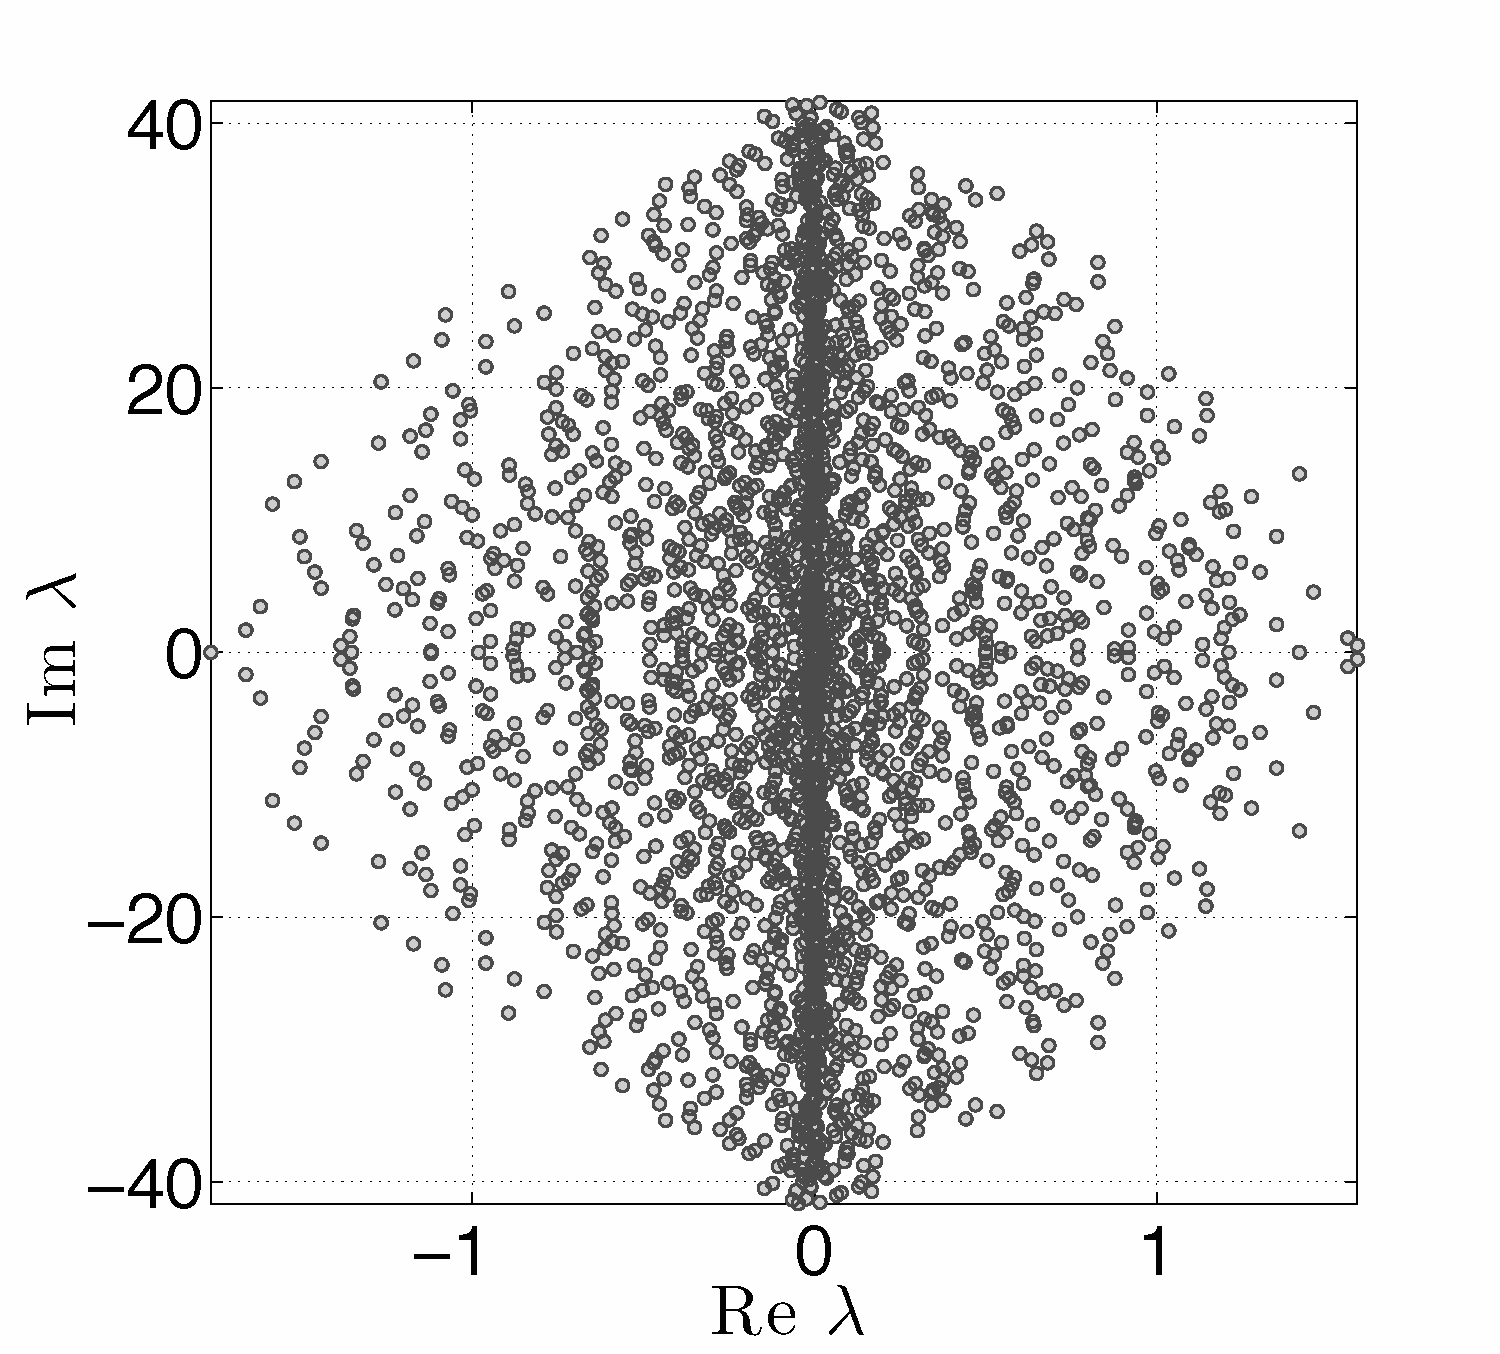
\includegraphics[width=1.0\textwidth]{figures/paper1/figures/cosine_bell/eigs_N4096_n101_noHV_SCALED.pdf}
	\caption{No Hyperviscosity}
	\label{fig:cosine_eigs_nohv}
\end{subfigure}
\begin{subfigure}[b]{0.45\textwidth}
	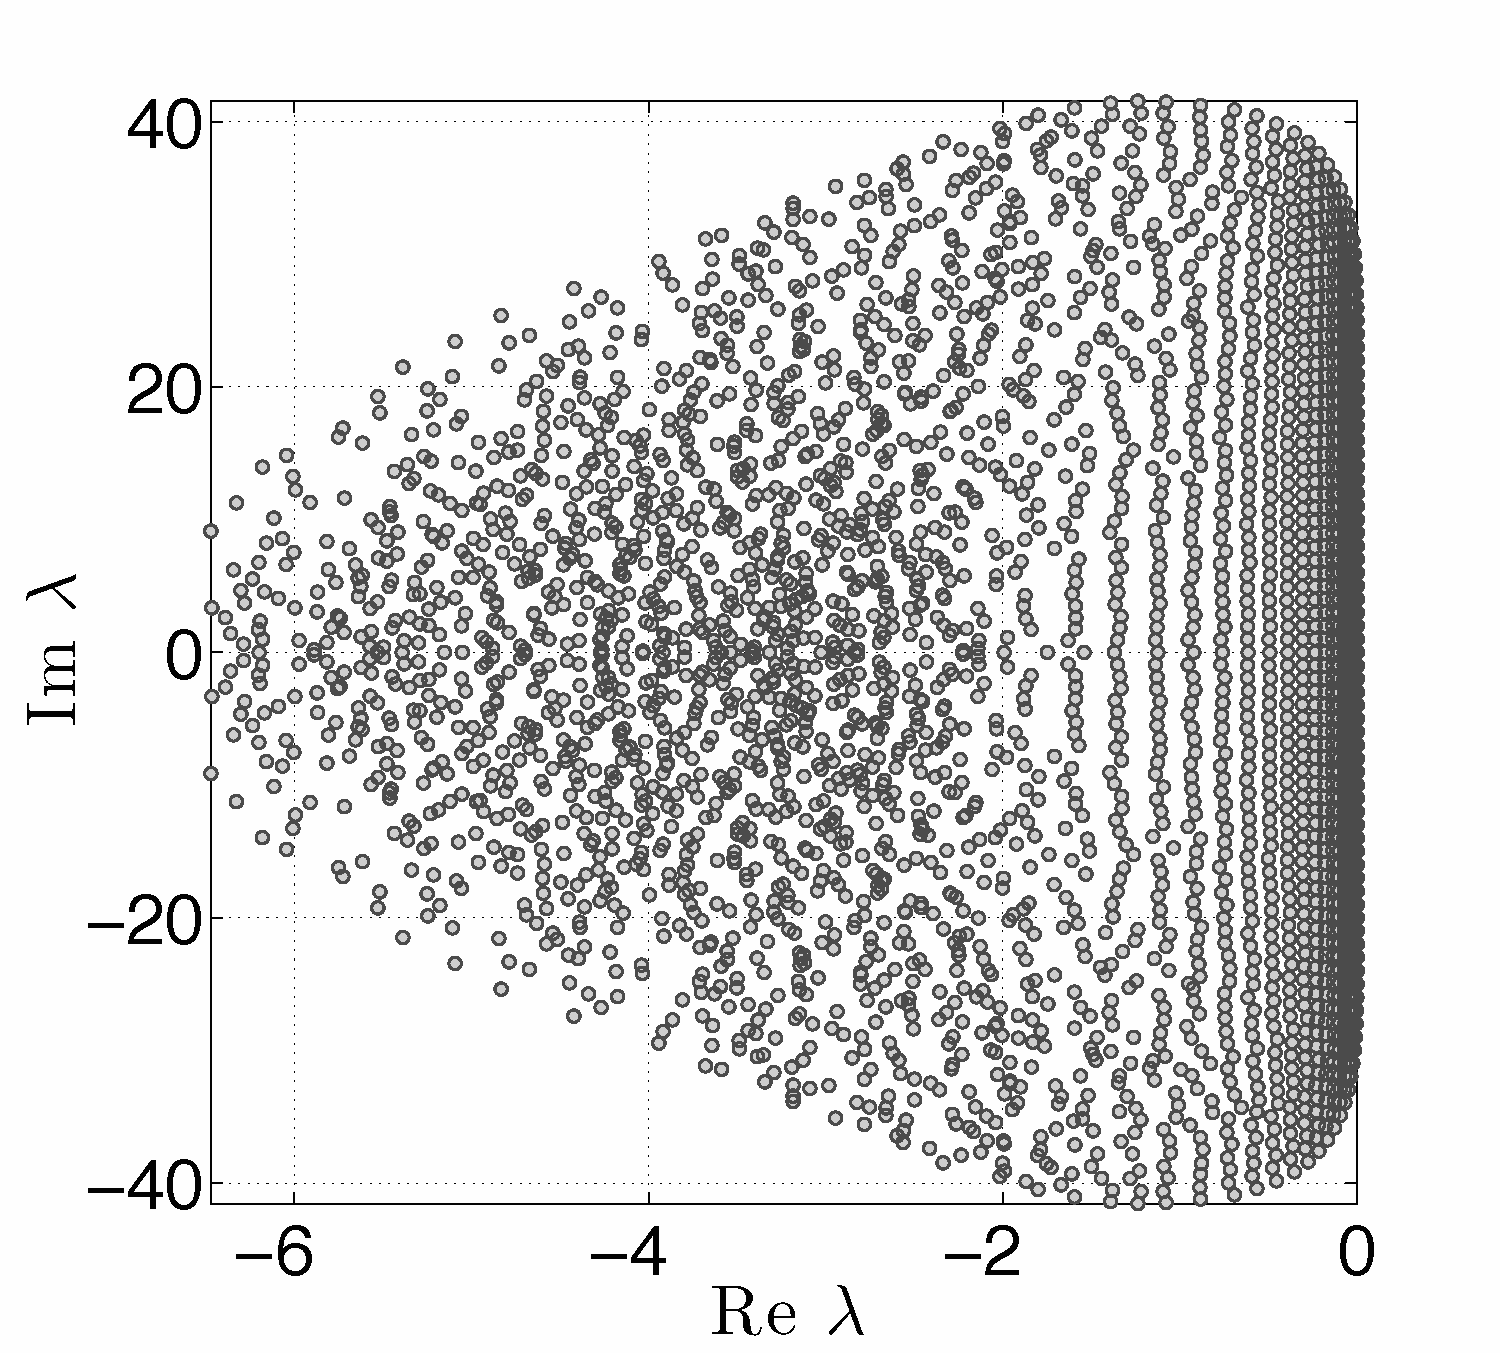
\includegraphics[width=1.0\textwidth]{figures/paper1/figures/cosine_bell/eigs_HV_N4096_n101_k8_gamma5e_m2_SCALED.pdf}
	\caption{With Hyperviscosity}
	\label{fig:cosine_eigs_hv}
\end{subfigure}
\caption{Eigenvalues of (\ref{eq:cosine_with_hyperviscosity}) for the cosine bell test case with $N=4096$ nodes, stencil size $n=101$, and $\epsilon = 3.5$. Left: no hyperviscosity. Right: hyperviscosity enabled with $k=8$ and $\gamma_c = 5*10^{-2}$. Eigenvalues are divided by $u_0$ to remove scaling effects of velocity.  
}
\label{fig:eig_cosine}
\end{center}
\end{figure}

\begin{figure}[ht!]
\begin{center}
\begin{subfigure}[b]{0.45\textwidth}
	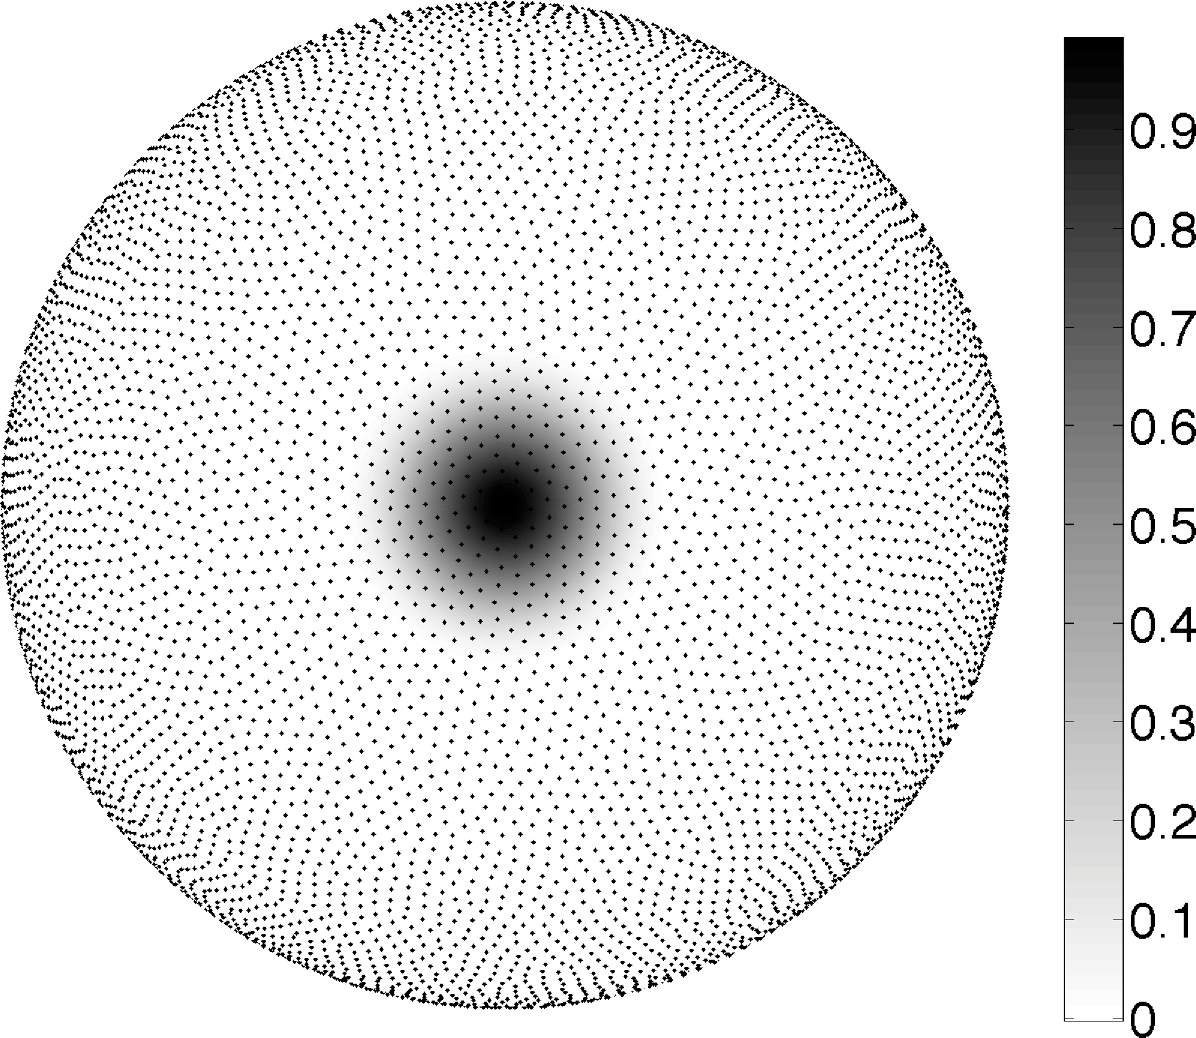
\includegraphics[width=1.0\textwidth]{figures/paper1/figures/cosine_bell/trimmed_ComputedSolution_ManualBar.pdf}
	\caption{10 Revolutions}
	\label{fig:cosine_approx}
\end{subfigure}
\begin{subfigure}[b]{0.45\textwidth}
	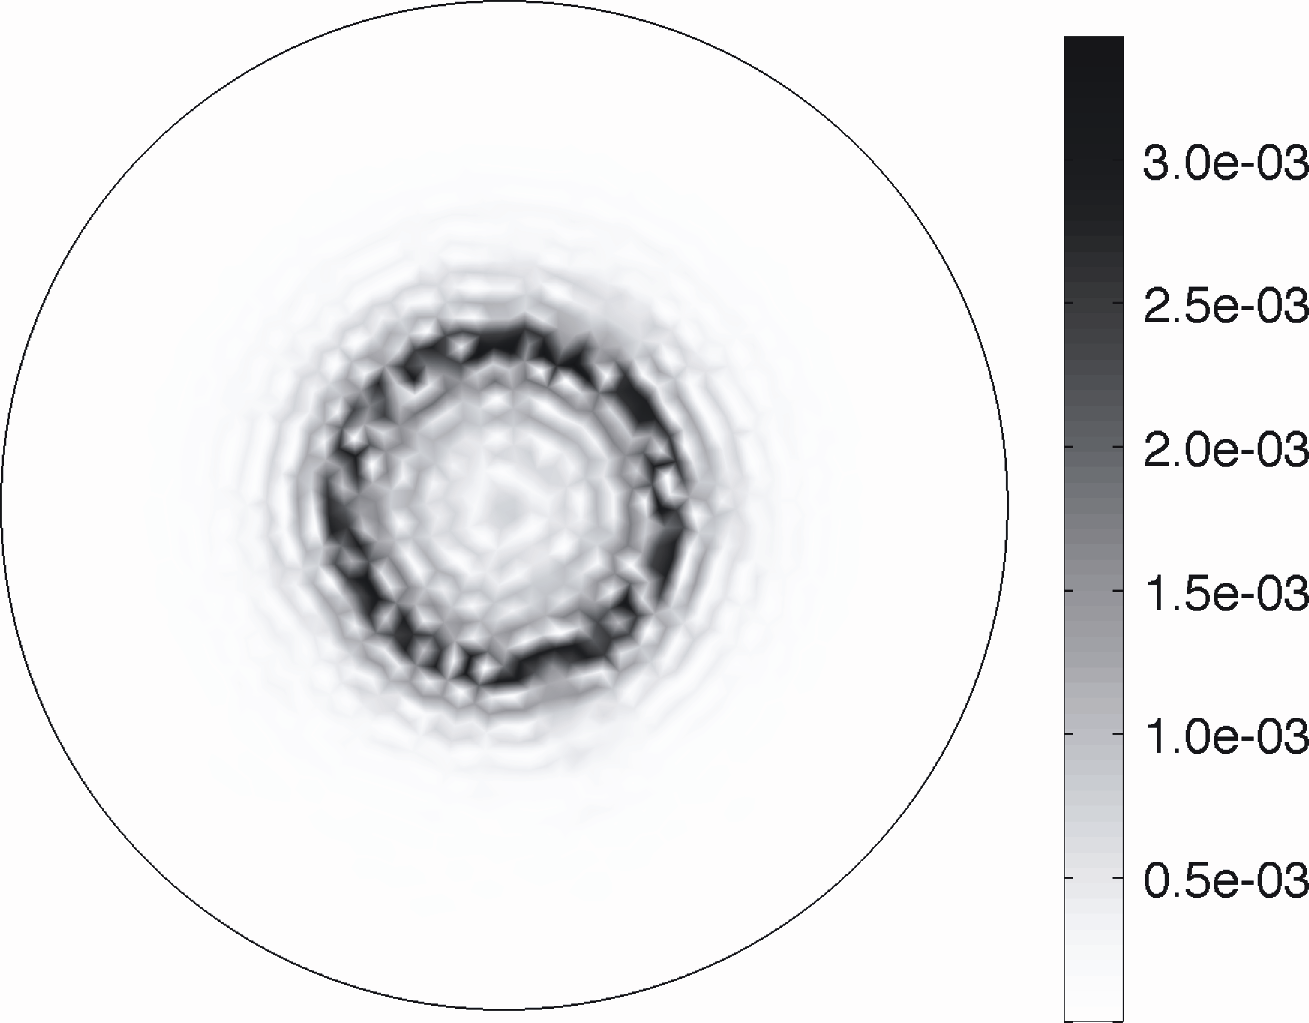
\includegraphics[width=1.0\textwidth]{figures/paper1/figures/cosine_bell/trimmed_Error_CoveredScale2.pdf}
	\caption{Absolute Error at $10$ Revolutions}
	\label{fig:cosine_abserror}
\end{subfigure}
\caption{Cosine bell solution after 10 revolutions with $N=10201$ nodes and stencil size $n=101$.
Hyperviscosity parameters are $k = 8$, $\gamma_c = 5(10^{-2})$. 
}
 \label{fig:cosine_10revs}
\end{center}
\end{figure}

Figure~\ref{fig:eig_cosine} compares eigenvalues of the DM for $N=4096$ nodes and stencil size $n=101$ before and after hyperviscosity is applied. To avoid scaling effects of velocity on the eigenvalues, they have been scaled by $1/u_0$.  The same approach as in the vortex roll-up case is used to determine the parameters for hyperviscosity and $\epsilon$. Our tuned parameters are presented in 
%\blue{However, note the difference in scale on the real axis compared to the vortex roll-up case; the initial range of the real part of the eigenvalues is approximately four orders of magnitude smaller. In this case, eigenvalues are more sensitive to the hyperviscosity filter. 
Table~\ref{tbl:cos_hv_params}.
% provides appropriate parameters for hyperviscosity in this test case. %, which reflect the difference in scale of $\gamma_c$ compared to Table~\ref{tbl:vortex_hv_params}.
%The parameters for hyperviscosity are dependent on $u_0$ 

%\clearpage

Figure~\ref{fig:cosine_10revs} shows the cosine bell transported ten full revolutions around the sphere. Without hyperviscosity, RBF-FD cannot complete a single revolution of the bell before instability takes over. However, adding hyperviscosity allows computation to extend to dozens or even thousands of revolutions and maintain stability (e.g., see \cite{FornbergLehto11}). After ten revolutions, the cosine bell is still intact. The majority of the absolute error (Figure~\ref{fig:cosine_abserror}) appears at the base of the $C^1$ bell where the discontinuity appears in the derivative. At ten revolutions, Figure~\ref{fig:conv_cosine_bell} illustrates the convergence of the RBF-FD method. All tests in Figure~\ref{fig:conv_cosine_bell} assume 1000 time-steps per revolution (i.e., $\Delta t = 1036.8$ seconds). 


\hl{Complete:}
17.28 minutes was a conservative step that allowed the problem to scale up to $N=27556$ nodes. Compare this to the conservative 30 minute time-step taken for $N=4096$ nodes in \cite{FlyerWright07}, which was already half necessary for DG and 8x less than necessary for both Spherical Harmonics and Double Fourier methods.\authnote{It would be good to quantify the appropriate $dt$ that would compare RBF-FD to their $N=4096$ case with global RBFs.} 


\begin{figure}[htbp]
\begin{center}
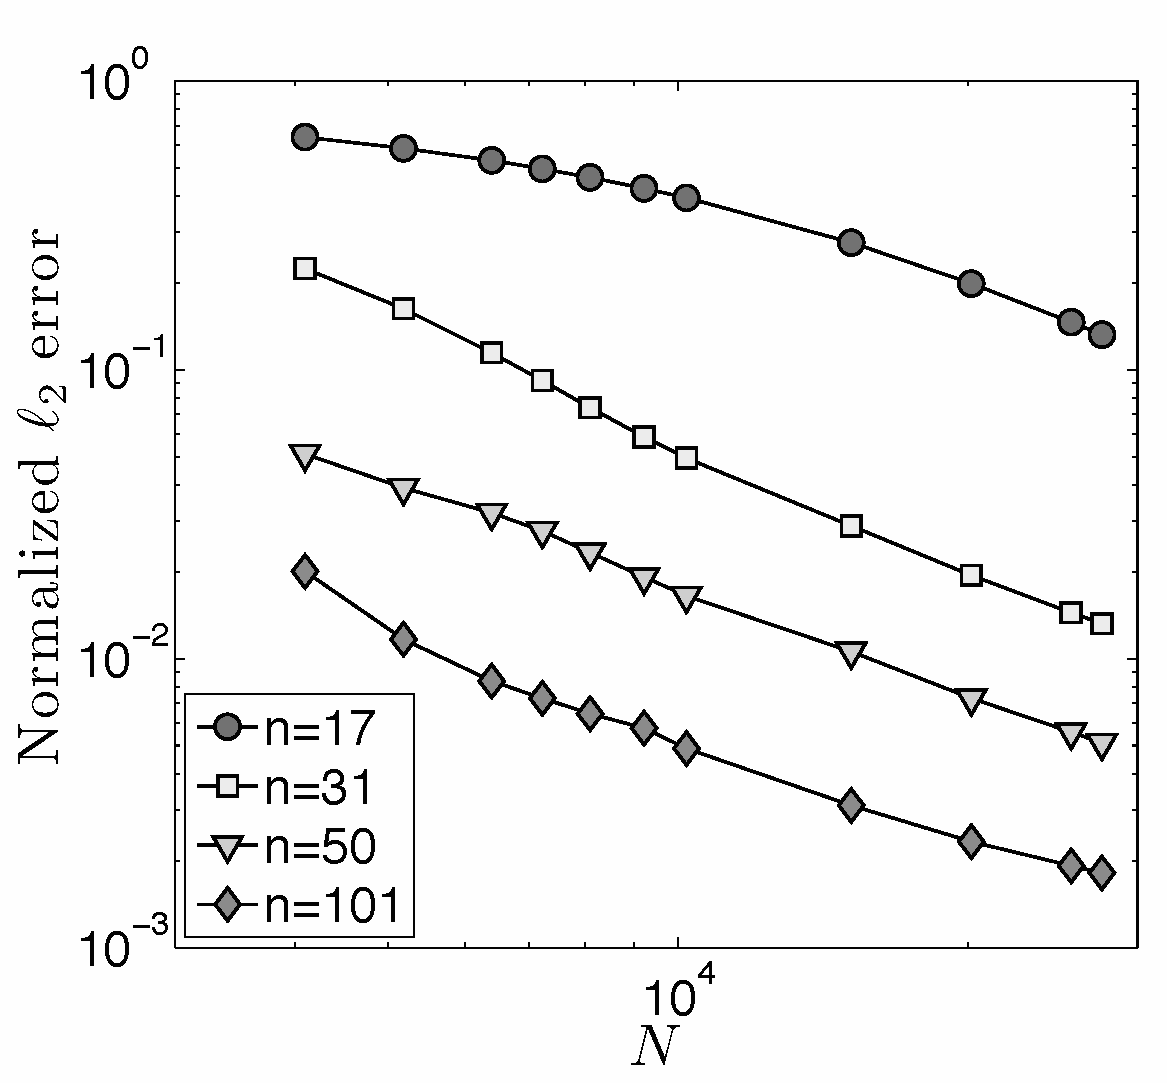
\includegraphics[width=3in]{figures/paper1/figures/cosine_bell/convergence_plot_hv.pdf}
\caption{Convergence plot for cosine bell advection. Normalized $\ell_2$ error at 10 revolutions with hyperviscosity enabled. }
\label{fig:conv_cosine_bell}
\end{center}
\end{figure}


\section{Fragments (integrate above)}
To verify our multi-CPU and multi-CPU+GPU implementations, two hyperbolic PDEs on the surface of the sphere are tested. For both cases a spherical coordinate system is used in terms of latitude $\lambda$ and longitude $\theta$:
\begin{eqnarray*} 
x & = & \rho \cos \lambda \cos \theta, 	\\
y & = & \rho \sin \lambda \cos \theta, 		\\
z & = & \rho \sin \theta.		
\end{eqnarray*}

Node sets are the Maximum Determinant point distributions on the sphere \cite{Sloan2003} consistent with previously published results (see e.g., \cite{Flyer2007} and \cite{Fornberg2011b}).

Hyperviscosity parameters $\gamma_c$ and $k$ depend on the RHS of the PDE. 
For this test case, hyperviscosity scaling parameters are listed in Table~\ref{tbl:vortex_hv_params}. Linear functions to choose the RBF support parameter $\epsilon$ are also provided. The parameters $\gamma_c$ and $k$ were obtained via trial-and-error parameter searching on $N=4096$ nodes. The goal when choosing parameters is to push all eigenvalues to the left half-plane, and then tweak $\gamma_c$ up or down to condense the eigenvalues as near to the imaginary axis as possible. We try to keep the range of filtered eigenvalue real parts within twice the width of the unfiltered range, so hyperviscosity does not cause too much diffusion in the solution. 

For the cosine bell we use the initial conditions
\begin{equation*}
h  = 
\begin{cases} 
\frac{h_0}{2} (1 + \cos(\frac{\pi \rho}{R})  & \rho \le R  \\
 0 &  \rho \geq R 
\end{cases}
\end{equation*}
where the bell of radius $R = \frac{a}{3}$ is centered at $(\lambda_c, \theta_c)$ and provided by the expression,
\begin{eqnarray*}
\rho = a \arccos( \sin \theta_{c} \sin \theta + \cos \theta_{c} \cos \theta \cos (\lambda - \lambda_{c}) ).
\end{eqnarray*}
We assume $a = 1$, $h_0 = 1$, and $(\lambda_c, \theta_c) = (^{3\pi}/_{2}, 0)$. The angle $\alpha =\ ^{\pi}/_{2}$ is chosen to transport the bell over the poles of the coordinate system, and $u_0 =\ ^{2 \pi a}/_{1036800}$. 

\authnote{Include figures from NCL or Paraview}


\section{Elliptic}
 

need chapter stating publications and talks, internships, developer status
need Survey of goals stated in prospectus and whether they were completed or not (Probably part of slides, not actual dissertation)

\makeatletter
\@ifundefined{standalonetrue}{\newif\ifstandalone}{}
\@ifundefined{section}{\standalonetrue}{\standalonefalse}
\makeatother
\ifstandalone
\documentclass{report}

\usepackage{textcase}
%\usepackage{hyperref}
%\hypersetup{breaklinks=true}


% Added packages
\usepackage[usenames]{color}
\usepackage{amsfonts, amsmath, amssymb, graphics}

% NOTE: bibentry MUST appear before the hyperref or build will fail
\usepackage{bibentry}
\nobibliography*
\usepackage[square,sort,comma,numbers]{natbib}
  
\usepackage{float}
\usepackage[
	hidelinks,%
    %hyperindex=true,		% Make numbers of index links as well
   	backref=page, 		% Provide page listing where refs occur in the bibliography
	%breaklinks=true,
    %colorlinks,%
    %citecolor=green,%
    %filecolor=blue,%
    %linkcolor=red,%
    %urlcolor=red, 
]{hyperref}

\usepackage{dsfont}
%%%% USEPACKAGES for MACROS %%%%%
\usepackage{algpseudocode}
\usepackage[chapter]{algorithm}
%\usepackage{caption}
\usepackage{subcaption}
\usepackage{url}

\usepackage{array}
\usepackage{arydshln}
\usepackage{multirow}
\usepackage{multicol}
%\usepackage[section]{placeins}

\usepackage[usenames,dvipsnames]{color}
%\usepackage[english]{babel}
\usepackage{tabularx}
\usepackage{soul}
\usepackage{xparse}
\usepackage{listings}
%\usepackage[normalem]{ulem}



%%%%%%%%%%%%%%%
% Show a list of items "todo" or "done" 
% USAGE: 
% \begin{todolist} 
% 	\todo Something not finished
% 	\done Something finished
% \end{todolist} 
\newenvironment{todolist}{%
  \begin{list}{}{}% whatever you want the list to be
  \let\olditem\item
  \renewcommand\item{\olditem \textcolor{red}{(TODO)}: }
  \newcommand\todo{\olditem \textcolor{red}{(TODO)}: }
   \newcommand\done{\olditem \textcolor{ForestGreen}{(DONE)}: }
}{%
  \end{list}
} 
%%%%%%%%%%%%%%%

%%%%%%%%%%%%%%%
% Show a Author's Note
% USAGE: 
% \incomplete[Optional footnote message to further clarify note]{The text which is currently not finished}
\DeclareDocumentCommand \incomplete{ o m }
{%
\IfNoValueTF {#1}
{\textcolor{red}{Incomplete: \ul{#2}}} 
{\textcolor{red}{Incomplete: \ul{#2}}\footnote{Comment: #1}}%
}
%%%%%%%%%%%%%%%



%%%%%%%%%%%%%%%
% Show a Author's Note
% USAGE: 
% \authnote[Optional footnote message to further clarify note]{The note to your readers}
\DeclareDocumentCommand \authnote { o m }
{%
\IfNoValueTF {#1}
{\textcolor{blue}{Author's Note: \ul{#2}}} 
{\textcolor{blue}{Author's Note: \ul{#2}}\footnote{Comment: #1}}%
}
%%%%%%%%%%%%%%%



%%%%%%%%%%%%%%%
% Strike out text that doesn't belong in the paper
% USAGE: 
% \strike[Optional footnote to state why it doesn't belong]{Text to strike out}
\DeclareDocumentCommand \strike { o m }
{%
\setstcolor{Red}
\IfNoValueTF {#1}
{\textcolor{Gray}{\st{#2}}} 
{\textcolor{Gray}{\st{#2}}\footnote{Comment: #1}}%
}
%%%%%%%%%%%%%%%

\definecolor{light-gray}{gray}{0.95}

\newcommand{\cbox}[3]{
\ \\
\fcolorbox{#1}{#2}{
\parbox{\textwidth}{
#3
}
}
}

% Setup an environment similar to verbatim but which will highlight any bash commands we have
\lstnewenvironment{unixcmds}[0]
{
%\lstset{language=bash,frame=shadowbox,rulesepcolor=\color{blue}}
\lstset{ %
language=sh,		% Language
basicstyle=\ttfamily,
backgroundcolor=\color{light-gray}, 
rulecolor=\color{blue},
%frame=tb, 
columns=fullflexible,
%framexrightmargin=-.2\textwidth,
linewidth=0.8\textwidth,
breaklines=true,
%prebreak=/, 
  prebreak = \raisebox{0ex}[0ex][0ex]{\ensuremath{\hookleftarrow}},
%basicstyle=\footnotesize,       % the size of the fonts that are used for the code
%numbers=left,                   % where to put the line-numbers
%numberstyle=\footnotesize,      % the size of the fonts that are used for the line-numbers
%stepnumber=2,                   % the step between two line-numbers. If it's 1 each line 
                                % will be numbered
%numbersep=5pt,                  % how far the line-numbers are from the code
showspaces=false,               % show spaces adding particular underscores
showstringspaces=false,         % underline spaces within strings
showtabs=false,                 % show tabs within strings adding particular underscores
frame=single,	                % adds a frame around the code
tabsize=2,	                % sets default tabsize to 2 spaces
captionpos=b,                   % sets the caption-position to bottom
breakatwhitespace=false,        % sets if automatic breaks should only happen at whitespace
}
} { }

% Setup an environment similar to verbatim but which will highlight any bash commands we have
\lstnewenvironment{cppcode}[1]
{
%\lstset{language=bash,frame=shadowbox,rulesepcolor=\color{blue}}
\lstset{ %
	backgroundcolor=\color{light-gray}, 
	rulecolor=\color[rgb]{0.133,0.545,0.133},
	tabsize=4,
	language=[GNU]C++,
%	basicstyle=\ttfamily,
        basicstyle=\scriptsize,
        upquote=true,
        aboveskip={1.5\baselineskip},
        columns=fullflexible,
        %framexrightmargin=-.1\textwidth,
       %framexleftmargin=6mm,
        showstringspaces=false,
        extendedchars=true,
        breaklines=true,
        prebreak = \raisebox{0ex}[0ex][0ex]{\ensuremath{\hookleftarrow}},
        frame=single,
        showtabs=false,
        showspaces=false,
        showstringspaces=false,
        numbers=left,                   % where to put the line-numbers
	numberstyle=\footnotesize,      % the size of the fonts that are used for the line-numbers
	stepnumber=4,                   % the step between two line-numbers. If it's 1 each line 
                                % will be numbered
	firstnumber=#1,
         numbersep=5pt,                  % how far the line-numbers are from the code
        identifierstyle=\ttfamily,
        keywordstyle=\color[rgb]{0,0,1},
        commentstyle=\color[rgb]{0.133,0.545,0.133},
        stringstyle=\color[rgb]{0.627,0.126,0.941},
}
} { }

% Setup an environment similar to verbatim but which will highlight any bash commands we have
\lstnewenvironment{mcode}[1]
{
\lstset{ %
	backgroundcolor=\color{light-gray}, 
	rulecolor=\color[rgb]{0.133,0.545,0.133},
	tabsize=4,
	language=Matlab,
%	basicstyle=\ttfamily,
        basicstyle=\scriptsize,
        upquote=true,
        aboveskip={1.5\baselineskip},
        columns=fullflexible,
        %framexrightmargin=-.1\textwidth,
       %framexleftmargin=6mm,
        showstringspaces=false,
        extendedchars=true,
        breaklines=true,
        prebreak = \raisebox{0ex}[0ex][0ex]{\ensuremath{\hookleftarrow}},
        frame=single,
        showtabs=false,
        showspaces=false,
        showstringspaces=false,
        numbers=left,                   % where to put the line-numbers
	numberstyle=\footnotesize,      % the size of the fonts that are used for the line-numbers
	stepnumber=4,                   % the step between two line-numbers. If it's 1 each line 
                                % will be numbered
	firstnumber=#1,
         numbersep=5pt,                  % how far the line-numbers are from the code
        identifierstyle=\ttfamily,
        keywordstyle=\color[rgb]{0,0,1},
        commentstyle=\color[rgb]{0.133,0.545,0.133},
        stringstyle=\color[rgb]{0.627,0.126,0.941},
}
} { }

\newcommand{\inputmcode}[1]{%
\lstset{ %
	backgroundcolor=\color{light-gray},  %
	rulecolor=\color[rgb]{0.133,0.545,0.133}, %
	tabsize=4, %
	language=Matlab, %
%	basicstyle=\ttfamily,
        basicstyle=\scriptsize, %
        %        upquote=true,
        aboveskip={1.5\baselineskip}, %
        columns=fullflexible, %
        %framexrightmargin=-.1\textwidth,
       %framexleftmargin=6mm,
        showstringspaces=false, %
        extendedchars=true, %
        breaklines=true, %
        prebreak = \raisebox{0ex}[0ex][0ex]{\ensuremath{\hookleftarrow}}, %
        frame=single, %
        showtabs=false, %
        showspaces=false, %
        showstringspaces=false,%
        numbers=left,                   % where to put the line-numbers
	numberstyle=\footnotesize,      % the size of the fonts that are used for the line-numbers
	stepnumber=4,                   % the step between two line-numbers. If it's 1 each line 
                                % will be numbered
         numbersep=5pt,                  % how far the line-numbers are from the code
        identifierstyle=\ttfamily, %
        keywordstyle=\color[rgb]{0,0,1}, %
        commentstyle=\color[rgb]{0.133,0.545,0.133}, %
        stringstyle=\color[rgb]{0.627,0.126,0.941} %
}
\lstinputlisting{#1}%
}

%\lstset{ %
%	backgroundcolor=\color{light-gray}, 
%	rulecolor=\color[rgb]{0.133,0.545,0.133},
%	tabsize=4,
%	language=Matlab,
%%	basicstyle=\ttfamily,
%        basicstyle=\scriptsize,
%        upquote=true,
%        aboveskip={1.5\baselineskip},
%        columns=fullflexible,
%        %framexrightmargin=-.1\textwidth,
%       %framexleftmargin=6mm,
%        showstringspaces=false,
%        extendedchars=true,
%        breaklines=true,
%        prebreak = \raisebox{0ex}[0ex][0ex]{\ensuremath{\hookleftarrow}},
%        frame=single,
%        showtabs=false,
%        showspaces=false,
%        showstringspaces=false,
%        numbers=left,                   % where to put the line-numbers
%	numberstyle=\footnotesize,      % the size of the fonts that are used for the line-numbers
%	stepnumber=4,                   % the step between two line-numbers. If it's 1 each line 
%                                % will be numbered
%	firstnumber=#1,
%         numbersep=5pt,                  % how far the line-numbers are from the code
%        identifierstyle=\ttfamily,
%        keywordstyle=\color[rgb]{0,0,1},
%        commentstyle=\color[rgb]{0.133,0.545,0.133},
%        stringstyle=\color[rgb]{0.627,0.126,0.941},
%}


\newcommand{\Laplacian}[1]{\nabla^2 #1}

% set of all nodes received and contained on GPU
\newcommand{\setAllNodes}[0]{\mathcal{G}}
% set of stencil centers on GPU
\newcommand{\setCenters}[0]{\mathcal{Q}}
% set of stencil centers with nodes in \setDepend
\newcommand{\setBoundary}[0]{\mathcal{B}}
% set of nodes received by other GPUs
\newcommand{\setDepend}[0]{\mathcal{R}}
% set of nodes sent to other GPUs
\newcommand{\setProvide}[0]{\mathcal{O}}


\newcommand{\toprule}[0]{\hline}
\newcommand{\midrule}[0]{\hline\hline}
\newcommand{\bottomrule}[0]{\hline}

\newcolumntype{C}{>{\centering\arraybackslash}b{1in}}
\newcolumntype{L}{>{\flushleft\arraybackslash}b{1.5in}}
\newcolumntype{R}{>{\flushright\arraybackslash}b{1.5in}}
\newcolumntype{D}{>{\flushright\arraybackslash}b{2.0in}}
\newcolumntype{E}{>{\flushright\arraybackslash}b{1.0in}}

\DeclareSymbolFont{AMSb}{U}{msb}{m}{n}
\DeclareMathSymbol{\N}{\mathbin}{AMSb}{"4E}
\DeclareMathSymbol{\Z}{\mathbin}{AMSb}{"5A}
\DeclareMathSymbol{\R}{\mathbin}{AMSb}{"52}
\DeclareMathSymbol{\Q}{\mathbin}{AMSb}{"51}
\DeclareMathSymbol{\PP}{\mathbin}{AMSb}{"50}
\DeclareMathSymbol{\I}{\mathbin}{AMSb}{"49}
%\DeclareMathSymbol{\C}{\mathbin}{AMSb}{"43}

%%%%%% VECTOR NORM: %%%%%%%
\newcommand{\vectornorm}[1]{\left|\left|#1\right|\right|}
\newcommand{\vnorm}[1]{\left|\left|#1\right|\right|}
\newcommand{\by}[0]{\times}
\newcommand{\vect}[1]{\mathbf{#1}}
%\newcommand{\mat}[1]{\mathbf{#1}} 

%\renewcommand{\vec}[1]{ \textbf{#1} }
%%%%%%%%%%%%%%%%%%%%%%

%%%%%%% THM, COR, DEF %%%%%%%
%\newtheorem{theorem}{Theorem}[section]
%\newtheorem{lemma}[theorem]{Lemma}
%\newtheorem{proposition}[theorem]{Proposition}
%\newtheorem{corollary}[theorem]{Corollary}
%\newenvironment{proof}[1][Proof]{\begin{trivlist}
%\item[\hskip \labelsep {\bfseries #1}]}{\end{trivlist}}
%\newenvironment{definition}[1][Definition]{\begin{trivlist}
%\item[\hskip \labelsep {\bfseries #1}]}{\end{trivlist}}
%\newenvironment{example}[1][Example]{\begin{trivlist}
%\item[\hskip \labelsep {\bfseries #1}]}{\end{trivlist}}
%\newenvironment{remark}[1][Remark]{\begin{trivlist}
%\item[\hskip \labelsep {\bfseries #1}]}{\end{trivlist}}
%\newcommand{\qed}{\nobreak \ifvmode \relax \else
%      \ifdim\lastskip<1.5em \hskip-\lastskip
%      \hskip1.5em plus0em minus0.5em \fi \nobreak
%      \vrule height0.75em width0.5em depth0.25em\fi}
%%%%%%%%%%%%%%%%%%%%%%

%
%\usepackage[algochapter]{algorithm2e}
%\usepackage[usenames]{color}
% colors to show the corrections
\newcommand{\red}[1]{\textbf{\textcolor{red}{#1}}}
\newcommand{\blue}[1]{\textbf{\textcolor{blue}{#1}}}
\newcommand{\cyan}[1]{\textbf{\textcolor{cyan}{#1}}}
\newcommand{\green}[1]{\textbf{\textcolor{green}{#1}}}
\newcommand{\magenta}[1]{\textbf{\textcolor{magenta}{#1}}}
\newcommand{\orange}[1]{\textbf{\textcolor{orange}{#1}}}
%%%%%%%%%% DK DK
% comments between authors
\newcommand{\toall}[1]{\textbf{\green{@@@ All: #1 @@@}}}
\newcommand{\toevan}[1]{\textbf{\red{*** Evan: #1 ***}}}
%\newcommand{\toevan}[1]{}  % USE FOR FINAL VERSION
\newcommand{\toe}[1]{\textbf{\red{*** Evan: #1 ***}}}
\newcommand{\tog}[1]{\textbf{\blue{*** Gordon: #1 ***}}}
%\newcommand{\togordon}[1]{\textbf{\blue{*** Gordon: #1 ***}}}
\renewcommand{\ge}[3]{{\textcolor{blue}{*** \textbf{Gordon:}\strike{#1} #2 ***}}\red{(#3)}}
\renewcommand{\ge}[3]{{\textcolor{blue}{#2}}}
\renewcommand{\ge}[3]{{\textcolor{Red}{#2}}}
\newcommand{\eb}[3]{{\textcolor{Red}{*** \textbf{Evan:}\strike{#1} #2 ***}}\red{(#3)}}
\renewcommand{\eb}[3]{{{\textcolor{Red}{#2}}}}
%\def\ge#1#2#3{}{\textbf{\blue{*** Gordon: #2 ***}}}{(#3)}
\newcommand{\gee}[1]{{\bf{\blue{{\em #1}}}}}
\newcommand{\old}[1]{}
\newcommand{\del}[1]{***#1*** }



% \DeclareMathOperator{\Sample}{Sample}
%\let\vaccent=\v % rename builtin command \v{} to \vaccent{}
%\renewcommand{\vec}[1]{\ensuremath{\mathbf{#1}}} % for vectors
\newcommand{\gv}[1]{\ensuremath{\mbox{\boldmath$ #1 $}}} 
% for vectors of Greek letters
\newcommand{\uv}[1]{\ensuremath{\mathbf{\hat{#1}}}} % for unit vector
\newcommand{\abs}[1]{\left| #1 \right|} % for absolute value
\newcommand{\avg}[1]{\left< #1 \right>} % for average
\let\underdot=\d % rename builtin command \d{} to \underdot{}
\renewcommand{\d}[2]{\frac{d #1}{d #2}} % for derivatives
\newcommand{\dd}[2]{\frac{d^2 #1}{d #2^2}} % for double derivatives
\newcommand{\pd}[2]{\frac{\partial #1}{\partial #2}} 
% for partial derivatives
\newcommand{\pdd}[2]{\frac{\partial^2 #1}{\partial #2^2}} 
\newcommand{\pdda}[3]{\frac{\partial^2 #1}{\partial #2 \partial #3}} 
% for double partial derivatives
\newcommand{\pdc}[3]{\left( \frac{\partial #1}{\partial #2}
 \right)_{#3}} % for thermodynamic partial derivatives
\newcommand{\ket}[1]{\left| #1 \right>} % for Dirac bras
\newcommand{\bra}[1]{\left< #1 \right|} % for Dirac kets
\newcommand{\braket}[2]{\left< #1 \vphantom{#2} \right|
 \left. #2 \vphantom{#1} \right>} % for Dirac brackets
\newcommand{\matrixel}[3]{\left< #1 \vphantom{#2#3} \right|
 #2 \left| #3 \vphantom{#1#2} \right>} % for Dirac matrix elements
\newcommand{\grad}[1]{\gv{\nabla} #1} % for gradient
\let\divsymb=\div % rename builtin command \div to \divsymb
\renewcommand{\div}[1]{\gv{\nabla} \cdot #1} % for divergence
\newcommand{\curl}[1]{\gv{\nabla} \times #1} % for curl
\let\baraccent=\= % rename builtin command \= to \baraccent
\renewcommand{\=}[1]{\stackrel{#1}{=}} % for putting numbers above =
\newcommand{\diffop}[1]{\mathcal{L}#1}
\newcommand{\boundop}[1]{\mathcal{B}#1}
\newcommand{\rvec}[0]{{\bf r}}

\newcommand{\Interior}[0]{\Omega}
\newcommand{\domain}[0]{\Omega}
%\newcommand{\Boundary}[0]{\partial \Omega}
\newcommand{\Boundary}[0]{\Gamma}

\newcommand{\on}[1]{\hskip1.5em \textrm{ on } #1}

\newcommand{\gemm}{\texttt{GEMM}}
\newcommand{\trmm}{\texttt{TRMM}}
\newcommand{\gesvd}{\texttt{GESVD}}
\newcommand{\geqrf}{\texttt{GEQRF}}


\newcommand{\minitab}[2][l]{\begin{tabular}{#1}#2\end{tabular}}
\newcommand{\comm}[1]{\textcolor{red}{\textit{#1}}}

\newcommand{\nfrac}[2]{
\nicefrac{#1}{#2}
%\frac{#1}{#2}
}

\usepackage{xparse}
\usepackage{soul}


%%%%%%%%%%%%%%%
% Show a Author's Note
% USAGE: 
% \incomplete[Optional footnote message to further clarify note]{The text which is currently not finished}
\DeclareDocumentCommand \incomplete{ o m }
{%
\IfNoValueTF {#1}
{\textcolor{red}{Incomplete: \ul{#2}}} 
{\textcolor{red}{Incomplete: \ul{#2}}\footnote{Comment: #1}}%
}
%%%%%%%%%%%%%%%



%%%%%%%%%%%%%%%
% Show a Author's Note
% USAGE: 
% \authnote[Optional footnote message to further clarify note]{The note to your readers}
\DeclareDocumentCommand \authnote { o m }
{%
\IfNoValueTF {#1}
{\textcolor{blue}{Author's Note: \ul{#2}}} 
{\textcolor{blue}{Author's Note: \ul{#2}}\footnote{Comment: #1}}%
}
%%%%%%%%%%%%%%%



%%%%%%%%%%%%%%%
% Strike out text that doesn't belong in the paper
% USAGE: 
% \strike[Optional footnote to state why it doesn't belong]{Text to strike out}
\DeclareDocumentCommand \strike { o m }
{%
\setstcolor{red}
\IfNoValueTF {#1}
{\textcolor{Gray}{\st{#2}}} 
{\textcolor{Gray}{\st{#2}}\footnote{Comment: #1}}%
}
%%%%%%%%%%%%%%%



%
% colors to show the corrections
\newcommand{\red}[1]{\textbf{\textcolor{red}{#1}}}
\newcommand{\blue}[1]{\textbf{\textcolor{blue}{#1}}}
\newcommand{\cyan}[1]{\textbf{\textcolor{cyan}{#1}}}
\newcommand{\green}[1]{\textbf{\textcolor{green}{#1}}}
\newcommand{\magenta}[1]{\textbf{\textcolor{magenta}{#1}}}
\newcommand{\orange}[1]{\textbf{\textcolor{orange}{#1}}}
%%%%%%%%%% DK DK
% comments between authors
\newcommand{\toall}[1]{\textbf{\green{@@@ All: #1 @@@}}}
\newcommand{\toevan}[1]{\textbf{\red{*** Evan: #1 ***}}}
%\newcommand{\toevan}[1]{}  % USE FOR FINAL VERSION
\newcommand{\toe}[1]{\textbf{\red{*** Evan: #1 ***}}}
\newcommand{\tog}[1]{\textbf{\blue{*** Gordon: #1 ***}}}
%\newcommand{\togordon}[1]{\textbf{\blue{*** Gordon: #1 ***}}}
\renewcommand{\ge}[3]{{\textcolor{blue}{*** \textbf{Gordon:}\strike{#1} #2 ***}}\red{(#3)}}
\renewcommand{\ge}[3]{{\textcolor{blue}{#2}}}
\renewcommand{\ge}[3]{{\textcolor{red}{#2}}}
\newcommand{\eb}[3]{{\textcolor{red}{*** \textbf{Evan:}\strike{#1} #2 ***}}\red{(#3)}}
\renewcommand{\eb}[3]{{{\textcolor{red}{#2}}}}
%\def\ge#1#2#3{}{\textbf{\blue{*** Gordon: #2 ***}}}{(#3)}
\newcommand{\gee}[1]{{\bf{\blue{{\em #1}}}}}
\newcommand{\old}[1]{}
\newcommand{\del}[1]{***#1*** }



% Rename  this file          misc_mac.tex
%----------------------------------------------------------------------
%%%%%%%%%%%%%%%%%%%%%%%%%%%%%%%%%%%%%%%%%%%%%%%%%%%%%%%%%%%%%%%%%%%%%%%%%%%%%%%
%
%	Math Symbols   Math Symbols   Math Symbols   Math Symbols   
%
%%%%%%%%%%%%%%%%%%%%%%%%%%%%%%%%%%%%%%%%%%%%%%%%%%%%%%%%%%%%%%%%%%%%%%%%%%%%%%%
\def\pmb#1{\setbox0=\hbox{$#1$}%
	\kern-.025em\copy0\kern-\wd0
	\kern.05em\copy0\kern-\wd0
	\kern-.025em\raise.0433em\box0}
\def\pmbf#1{\pmb#1}
\def\bfg#1{\pmb#1}

% BETTER VALUES FOR AUTOMATIC FIGURE PLACEMENT THAN THOSE PROVIDED BY 
% LATEX DEFAULTS.

\renewcommand{\textfloatsep}{1ex}
\renewcommand{\floatpagefraction}{0.9}
\renewcommand{\intextsep}{1ex}
\renewcommand{\topfraction}{.9}
\renewcommand{\bottomfraction}{.9}
\renewcommand{\textfraction}{.1}

% #1  position of floating figure (h|t|b|p)
% #1  EPS postscript file
% #2  size
% #3  caption

%usage of newfig:
%  \newfig{file.ps}{3in}{Fig1: this is a figure}

\input{epsf}
\def\newfig#1#2#3{
  \begin{figure}[htbp]
  \vspace{1ex}
  \setlength{\epsfxsize}{#2}
  \centerline{\epsfbox{#1}}
  \vspace{-.1in}\caption{\small #3}\break\vspace{.2in}
  \label{#1}
  \end{figure}
}

%usage of newfigtwo: 2 figures, vertically stacked
% \newfig
%	{file1.ps}
%	{file2.ps}
%	{width}
%	{vertical space}
%	{Caption}

\def\newfigtwo#1#2#3#4#5{
  \begin{figure}[htbp]
  \vspace{1ex}
  \setlength{\epsfxsize}{#3}
  \centerline{\epsfbox{#1}}
  \vspace{#4}
  \setlength{\epsfxsize}{#3}
  \centerline{\epsfbox{#2}}
  \vspace{-.1in}\caption{\small #5}\break\vspace{.2in}
  \label{#1}
  \end{figure}
}

\def\newfigh#1#2#3#4{  % add height specification
  \begin{figure}[htbp]
  \vspace{1ex}
  \setlength{\epsfxsize}{#2}
  \setlength{\epsfysize}{#4}
  \centerline{\epsfbox{#1}}
  \vspace{-.1in}\caption{\small #3}\break\vspace{.2in}
  \label{#1}
  \end{figure}
}

\def\herefig#1#2#3{
  \begin{figure}[h]
  \setlength{\epsfxsize}{#2}
  \centerline{\epsfbox{#1}}
  \caption{\small #3}
  \label{#1}
  \end{figure}
}

\def\etal{{{\em et~al.\,\,}}}
\def\note#1{\\ =====#1===== \\}
\def\FBOX#1{\ \\ \fbox{\begin{minipage}{5in}#1\end{minipage}}\\ }
\newcount\sectionno     \sectionno=0
\newcount\eqnum         \eqnum=0
\def\addeqno{\global\advance \eqnum by  1 }
\def\subeqno{\global\advance \eqnum by -1 }
%\def\eqn{\addeqno \eqno \hbox{(\number\sectionno.\number\eqnum)} }

\def\tildetilde#1{\tilde{\tilde{#1}}}
\def\barbar#1{\overbar{\overbar{#1}}}

\def\vsp#1{\vspace{#1 ex}}
\def\fpar{\hspace{\parindent}}
%
%  \pf : 2 arguments: numerator and denominator of partial derivative
%
\def\pf#1#2{{\frac{\partial{#1}}{\partial{#2}}}}
\def\pfs#1#2{{\partial_{#2}{#1}}}
\def\pftwo#1#2{{\frac{\partial^2{#1}}{\partial{#2}^2}}}
\def\pfxx#1#2{{\frac{\partial^2{#1}}{\partial{#2}^2}}}
%\def\pfxy#1#2{{\frac{\partial^2{#1}}{\partial{#2}\partial{#3}}}}
\def\pfn#1#2#3{{\frac{\partial^{#1}{#2}}{\partial{#3}^{#1}}}}
\def\df#1#2{{\frac{d{#1}}{d{#2}}}}
\def\dfn#1#2#3{{\frac{d^{#1}{#2}}{d{#3}^{#1}}}}
\def\Dt#1#2{\frac{D#1}{D#2}}
\def\dt#1#2{\frac{d#1}{d#2}}
\def\bld#1{{\bf #1}}
\def\pfp#1#2#3{\pf{}{#3}{\left(\frac{#1}{#2}\right)}}

\def\norm#1{\|#1\|}

%
% Graphic characters  (\dot already defined by TeX/LateX)
%
\def\dash{\rule[1.5pt]{2mm}{.3mm}\HS{.9mm}}
\def\dott{\rule[1.5pt]{.7mm}{.3mm}\HS{.7mm}}
\def\dashline{\dash\dash\dash}
\def\dotline{\dott\dott\dott\dott\dott\dott}
\def\dashdotline{\dash$\cdot$\HS{.9mm}\dash}
\def\solidline{\rule[2pt]{7mm}{.3mm}}
% 
% overcircle
%
\def\ovcircle#1{\buildrel{\circ}\over{#1}}
%\def\below#1#2{\buildrel{#2}\under{#1}}
%\def\above#1#2{\buildrel{#2}\over{#1}}
%
%  big parenthesis and brackets
%
\def\bigpar#1#2{{\left(\frac{#1}{#2}\right)}}
\def\bigbra#1#2{{\left\[\frac{#1}{#2}\right\]}}

\def\Lp{\left(}
\def\Rp{\right)}
\def\Lb{\left[}
\def\Rb{\right]}
\def\Ln{\left\langle}
\def\Rn{\right\rangle}
\def\Ld{\left.}
\def\Rd{\right.}
\def\Lv{\left|}
\def\Rv{\right|}
\def\Lbr{\left|}
\def\Rbr{\right|}
\def\lng{\langle}
\def\rng{\rangle}
\def\Lc{\left\{}
\def\Rc{\right\}}
%%% %

% Cannot be handled by Lyx
%\def\[{{[}}
%\def\]{{]}}

%
\def\eol{\nonumber \\}
\def\eolnonb{\nonumber\\}
\def\eolnb{\\}
\def\nonb{\nonumber}
\def\be{\begin{equation}}
\def\ee{\end{equation}}
\def\BEQNA{\begin{eqnarray}}
\def\EEQNA{\end{eqnarray}}
\def\eqa{&=&}
\def\beqna{\begin{eqnarray}}
\def\eeqna{\end{eqnarray}}
\def\bverb{\begin{verbatim}}
\def\everb{\end{verbatim}}
\def\VERB#1{\bverb #1 \everb}
\def\btbl{\begin{tabular}}
\def\etbl{\end{tabular}}
\def\bmini{\begin{minipage}[t]{5.5in}}
\def\emini{\end{minipage}}
\def\parray#1#2{\left(\begin{array}{#1}#2\end{array}\right)}
\def\barray#1#2{\left[\begin{array}{#1}#2\end{array}\right]}
\def\carray#1#2{\left\{\begin{array}{#1}#2\end{array}\right.}
\def\darray#1#2{\left|\begin{array}{#1}#2\end{array}\right|}

\def\BEGTABLE#1{\begin{table}[hbt]\vspace{2ex}\begin{center}\bmini\centering\btbl{#1}}
\def\ENDTABLE#1#2{\etbl\caption[#1]{#2}\EMINI\end{center}\vspace{2ex}\end{table}}

\def\bfltbl#1{\begin{table}[hbt]\vspace{2ex}\begin{center}\bmini\centering\btbl{#1}}
\def\efltbl#1#2{\etbl\caption[#1]{#2}\emini\end{center}\vspace{2ex}\end{table}}
\def\mcol{\multicolumn}
%
%  label equations with (#)
%
\def\reff#1{(\ref{#1})}
%
%  macros borrowed from viewgraph package
%

\newenvironment{LETTRS}[3]{\begin{letter}{#1}
\input{origin}\opening{Dear #2:}\input{#3}\closing{Sincerely yours,}\end{letter}}{\clearpage}

\newenvironment{VIEW}[1]{{\BC\Huge\bf #1 \EC}\LARGE\VS{.05in}}{\clearpage}

\def\RM#1{\rm{#1\ }}
\def\BV{\begin{VIEW}}
\def\EV{\end{VIEW}}

\def\NI{\noindent}

\def\VS{\vspace*}
\def\HS{\hspace*}
\def\IT{\item}

\def\BARR{\begin{array}}
\def\EARR{\end{array}}

\def\BPARR{\left(\begin{array}}
\def\EPARR{\end{array}\right)}

\def\BDET{\left|\begin{array}}
\def\EDET{\end{array}\right|}

\def\BDF{\begin{definition}}
\def\EDF{\end{definition}}

\def\BSU{\begin{block}{Summary}}
\def\ESU{\end{block}}

\def\BEX{\begin{example}}
\def\EEX{\end{example}}

\def\BTH{\begin{theorem}}
\def\ETH{\end{theorem}}

\def\BCO{\begin{corollary}}
\def\ECO{\end{corollary}}

\def\BPROOF{\begin{proof}}
\def\EPROOF{\end{proof}}

\def\BLM{\begin{lemma}}
\def\ELM{\end{lemma}}

\def\BEQ{\begin{equation}}
\def\EEQ{\end{equation}}

\def\BEQNNB{$$}
\def\EEQNNB{$$}

\def\BE{\begin{enumerate}}
\def\EE{\end{enumerate}}

\def\BD{\begin{description}}
\def\ED{\end{description}}

\def\BI{\begin{itemize}}
\def\EI{\end{itemize}}

\def\BC{\begin{center}}
\def\EC{\end{center}}

\def\BFIG{\begin{figure}}
\def\EFIG{\end{figure}}

\def\BTABB{\begin{tabbing}}
\def\ETABB{\end{tabbing}}

\def\BMINI{\begin{minipage}}
\def\EMINI{\end{minipage}}

\def\BTABLE{\begin{table}}
\def\ETABLE{\end{table}}

\def\BTABUL{\begin{tabular}}
\def\ETABUL{\end{tabular}}

\def\MCOL{\multicolumn}
\def\UL{\underline}
\def\ULL#1{\UL{\UL{#1}}}

\def\BDOC{\begin{document}}
\def\EDOC{\end{document}}

\def\EM#1{{\em #1\/}}
\def\FN{\footnote}

% Courtesy of Ugo Piomelli

\def\latexfig #1 #2 #3 #4 #5 {\ \vfill
\hfill\hbox to 0.05in{\vbox to #3truein{
         \special{psfile="#1" angle=270 hscale=100 
                  hoffset=#4 voffset=#5 vscale=100} }\hfill}
\hfill\vspace{-0.1in}        }

% #1 is the .ps filename
% #2 is not used in the present version
% #3 is the size of the white space left above the caption (in inches)
% #4 is the horizontal offset from some unknown reference point.
%    It is in 1/72 of an inch and is positive to the right.
% #5 is the vertical offset from some unknown reference point.
%    It is in 1/72 of an inch and is positive upwards.


\newcommand{\mathsym}[1]{{}}
\newcommand{\unicode}[1]{{}}
\newcommand{\ep}{\epsilon}
\newcommand{\vv}{\mathbf{v}}
\newcommand{\vu}{\mathbf{u}}
\newcommand{\vx}{\mathbf{x}}

\newcommand{\Laplacian}[1]{\nabla^2 #1}
\newcommand{\LaplaceBeltrami}[1]{\Delta_S #1}

% set of all nodes received and contained on GPU
\newcommand{\setAllNodes}[0]{\mathcal{G}}
% set of stencil centers on GPU
\newcommand{\setCenters}[0]{\mathcal{Q}}
% set of stencil centers with nodes in \setDepend
\newcommand{\setBoundary}[0]{\mathcal{B}}
% set of nodes received by other GPUs
\newcommand{\setDepend}[0]{\mathcal{R}}
% set of nodes sent to other GPUs
\newcommand{\setProvide}[0]{\mathcal{O}}





\usepackage{tabularx} 
\newcolumntype{C}{>{\centering\arraybackslash}b{1in}}
\newcolumntype{L}{>{\flushleft\arraybackslash}b{1.5in}}
\newcolumntype{R}{>{\flushright\arraybackslash}b{1.5in}}
\newcolumntype{D}{>{\flushright\arraybackslash}b{2.0in}}
\newcolumntype{E}{>{\flushright\arraybackslash}b{1.0in}}


 


%\usepackage{xcolor}

%\usepackage{refcheck}
% Sepia
%\definecolor{myBGcolor}{HTML}{F6F0D6}
%\definecolor{myTextcolor}{HTML}{4F452C}
% Dark
%\definecolor{myBGcolor}{HTML}{3E3535}
%\definecolor{myTextcolor}{HTML}{CFECEC}
%\color{myTextcolor}
%\pagecolor{myBGcolor}
 

\begin{document}
\fi

\chapter{Community Outreach}


\begin{itemize} 
        \item \bibentry{ErlebacherSauleFlyerBollig2013}
        \item \bibentry{BolligFlyerErlebacher2012}
%        \item \bibentry{BolligFlyerErlebacher2012b}
        \item \bibentry{BolligSIAMSEAS2012}     
        \item \bibentry{BolligXpo2013}. Also presented at: the Minnesota Supercomputing Institute Research Exhibition, Minneapolis, MN, April 2013
        \item \bibentry{BolligXpo2012}
        \item \bibentry{BolligAGU2011}              
        \item \bibentry{BolligMA2011}
\end{itemize}



\ifstandalone
\bibliographystyle{plain}
\bibliography{merged_references}
\end{document}
\else
\expandafter\endinput
\fi


%\chapter{Review}
%\begin{itemize} 
%	\item Review of the Literature (don’t make the mistake of reviewing after rather than before data collection in qualitative studies)
%	\item The more references the better
%	\item All relevant, reliable, and recent studies be included
%	\item Organization is critical 
%	\item Compare, contrast, and evaluate previous studies
%\end{itemize}
%
%\chapter{Research Methodology}
%\begin{itemize} 
%	\item Research Perspective: type of methodology and why it is the best way to answer your research question
%	\item Context and Access: where, when, and how you will find participants 
% 	\item Instrumentation: include copy in appendix or in text if using survey or interview questions
% 	\item Procedure: be specific so a reader could imitate your study 
% 	\item Data Analysis: again, specific down to the computer program used for statistics
% 	\item Qualitative methods
% 	\item Data Sources
% 	\item Data Collection
% 	\item Data Analysis
% 	\item Verification
% 	\item Ethical Considerations
%\end{itemize} 
%
%\chapter{Findings}
%\begin{itemize} 
%	\item Research Findings (Will be regularly updated)
%	\item Presentation of Data (Graphs, charts, tables, etc)
%	\item Timings, Convergence Rates, etc.
%\end{itemize} 
%
%\chapter{Summary}
%\begin{itemize} 
%\item Summary (what should readers find in document)
%\item Conclusions (what are the improvements made, what algorithms are demonstrated effective?)
%\item Discussion
%\item Suggestions for future research
%\end{itemize} 
%%\makeatletter
\@ifundefined{standalonetrue}{\newif\ifstandalone}{}
\@ifundefined{section}{\standalonetrue}{\standalonefalse}
\makeatother
\ifstandalone
\documentclass[11pt]{report}
\usepackage{textcase}
%\usepackage{hyperref}
%\hypersetup{breaklinks=true}


% Added packages
\usepackage[usenames]{color}
\usepackage{amsfonts, amsmath, amssymb, graphics}

% NOTE: bibentry MUST appear before the hyperref or build will fail
\usepackage{bibentry}
\nobibliography*
\usepackage[square,sort,comma,numbers]{natbib}
  
\usepackage{float}
\usepackage[
	hidelinks,%
    %hyperindex=true,		% Make numbers of index links as well
   	backref=page, 		% Provide page listing where refs occur in the bibliography
	%breaklinks=true,
    %colorlinks,%
    %citecolor=green,%
    %filecolor=blue,%
    %linkcolor=red,%
    %urlcolor=red, 
]{hyperref}

\usepackage{dsfont}
%%%% USEPACKAGES for MACROS %%%%%
\usepackage{algpseudocode}
\usepackage[chapter]{algorithm}
%\usepackage{caption}
\usepackage{subcaption}
\usepackage{url}

\usepackage{array}
\usepackage{arydshln}
\usepackage{multirow}
\usepackage{multicol}
%\usepackage[section]{placeins}

\usepackage[usenames,dvipsnames]{color}
%\usepackage[english]{babel}
\usepackage{tabularx}
\usepackage{soul}
\usepackage{xparse}
\usepackage{listings}
%\usepackage[normalem]{ulem}



%%%%%%%%%%%%%%%
% Show a list of items "todo" or "done" 
% USAGE: 
% \begin{todolist} 
% 	\todo Something not finished
% 	\done Something finished
% \end{todolist} 
\newenvironment{todolist}{%
  \begin{list}{}{}% whatever you want the list to be
  \let\olditem\item
  \renewcommand\item{\olditem \textcolor{red}{(TODO)}: }
  \newcommand\todo{\olditem \textcolor{red}{(TODO)}: }
   \newcommand\done{\olditem \textcolor{ForestGreen}{(DONE)}: }
}{%
  \end{list}
} 
%%%%%%%%%%%%%%%

%%%%%%%%%%%%%%%
% Show a Author's Note
% USAGE: 
% \incomplete[Optional footnote message to further clarify note]{The text which is currently not finished}
\DeclareDocumentCommand \incomplete{ o m }
{%
\IfNoValueTF {#1}
{\textcolor{red}{Incomplete: \ul{#2}}} 
{\textcolor{red}{Incomplete: \ul{#2}}\footnote{Comment: #1}}%
}
%%%%%%%%%%%%%%%



%%%%%%%%%%%%%%%
% Show a Author's Note
% USAGE: 
% \authnote[Optional footnote message to further clarify note]{The note to your readers}
\DeclareDocumentCommand \authnote { o m }
{%
\IfNoValueTF {#1}
{\textcolor{blue}{Author's Note: \ul{#2}}} 
{\textcolor{blue}{Author's Note: \ul{#2}}\footnote{Comment: #1}}%
}
%%%%%%%%%%%%%%%



%%%%%%%%%%%%%%%
% Strike out text that doesn't belong in the paper
% USAGE: 
% \strike[Optional footnote to state why it doesn't belong]{Text to strike out}
\DeclareDocumentCommand \strike { o m }
{%
\setstcolor{Red}
\IfNoValueTF {#1}
{\textcolor{Gray}{\st{#2}}} 
{\textcolor{Gray}{\st{#2}}\footnote{Comment: #1}}%
}
%%%%%%%%%%%%%%%

\definecolor{light-gray}{gray}{0.95}

\newcommand{\cbox}[3]{
\ \\
\fcolorbox{#1}{#2}{
\parbox{\textwidth}{
#3
}
}
}

% Setup an environment similar to verbatim but which will highlight any bash commands we have
\lstnewenvironment{unixcmds}[0]
{
%\lstset{language=bash,frame=shadowbox,rulesepcolor=\color{blue}}
\lstset{ %
language=sh,		% Language
basicstyle=\ttfamily,
backgroundcolor=\color{light-gray}, 
rulecolor=\color{blue},
%frame=tb, 
columns=fullflexible,
%framexrightmargin=-.2\textwidth,
linewidth=0.8\textwidth,
breaklines=true,
%prebreak=/, 
  prebreak = \raisebox{0ex}[0ex][0ex]{\ensuremath{\hookleftarrow}},
%basicstyle=\footnotesize,       % the size of the fonts that are used for the code
%numbers=left,                   % where to put the line-numbers
%numberstyle=\footnotesize,      % the size of the fonts that are used for the line-numbers
%stepnumber=2,                   % the step between two line-numbers. If it's 1 each line 
                                % will be numbered
%numbersep=5pt,                  % how far the line-numbers are from the code
showspaces=false,               % show spaces adding particular underscores
showstringspaces=false,         % underline spaces within strings
showtabs=false,                 % show tabs within strings adding particular underscores
frame=single,	                % adds a frame around the code
tabsize=2,	                % sets default tabsize to 2 spaces
captionpos=b,                   % sets the caption-position to bottom
breakatwhitespace=false,        % sets if automatic breaks should only happen at whitespace
}
} { }

% Setup an environment similar to verbatim but which will highlight any bash commands we have
\lstnewenvironment{cppcode}[1]
{
%\lstset{language=bash,frame=shadowbox,rulesepcolor=\color{blue}}
\lstset{ %
	backgroundcolor=\color{light-gray}, 
	rulecolor=\color[rgb]{0.133,0.545,0.133},
	tabsize=4,
	language=[GNU]C++,
%	basicstyle=\ttfamily,
        basicstyle=\scriptsize,
        upquote=true,
        aboveskip={1.5\baselineskip},
        columns=fullflexible,
        %framexrightmargin=-.1\textwidth,
       %framexleftmargin=6mm,
        showstringspaces=false,
        extendedchars=true,
        breaklines=true,
        prebreak = \raisebox{0ex}[0ex][0ex]{\ensuremath{\hookleftarrow}},
        frame=single,
        showtabs=false,
        showspaces=false,
        showstringspaces=false,
        numbers=left,                   % where to put the line-numbers
	numberstyle=\footnotesize,      % the size of the fonts that are used for the line-numbers
	stepnumber=4,                   % the step between two line-numbers. If it's 1 each line 
                                % will be numbered
	firstnumber=#1,
         numbersep=5pt,                  % how far the line-numbers are from the code
        identifierstyle=\ttfamily,
        keywordstyle=\color[rgb]{0,0,1},
        commentstyle=\color[rgb]{0.133,0.545,0.133},
        stringstyle=\color[rgb]{0.627,0.126,0.941},
}
} { }

% Setup an environment similar to verbatim but which will highlight any bash commands we have
\lstnewenvironment{mcode}[1]
{
\lstset{ %
	backgroundcolor=\color{light-gray}, 
	rulecolor=\color[rgb]{0.133,0.545,0.133},
	tabsize=4,
	language=Matlab,
%	basicstyle=\ttfamily,
        basicstyle=\scriptsize,
        upquote=true,
        aboveskip={1.5\baselineskip},
        columns=fullflexible,
        %framexrightmargin=-.1\textwidth,
       %framexleftmargin=6mm,
        showstringspaces=false,
        extendedchars=true,
        breaklines=true,
        prebreak = \raisebox{0ex}[0ex][0ex]{\ensuremath{\hookleftarrow}},
        frame=single,
        showtabs=false,
        showspaces=false,
        showstringspaces=false,
        numbers=left,                   % where to put the line-numbers
	numberstyle=\footnotesize,      % the size of the fonts that are used for the line-numbers
	stepnumber=4,                   % the step between two line-numbers. If it's 1 each line 
                                % will be numbered
	firstnumber=#1,
         numbersep=5pt,                  % how far the line-numbers are from the code
        identifierstyle=\ttfamily,
        keywordstyle=\color[rgb]{0,0,1},
        commentstyle=\color[rgb]{0.133,0.545,0.133},
        stringstyle=\color[rgb]{0.627,0.126,0.941},
}
} { }

\newcommand{\inputmcode}[1]{%
\lstset{ %
	backgroundcolor=\color{light-gray},  %
	rulecolor=\color[rgb]{0.133,0.545,0.133}, %
	tabsize=4, %
	language=Matlab, %
%	basicstyle=\ttfamily,
        basicstyle=\scriptsize, %
        %        upquote=true,
        aboveskip={1.5\baselineskip}, %
        columns=fullflexible, %
        %framexrightmargin=-.1\textwidth,
       %framexleftmargin=6mm,
        showstringspaces=false, %
        extendedchars=true, %
        breaklines=true, %
        prebreak = \raisebox{0ex}[0ex][0ex]{\ensuremath{\hookleftarrow}}, %
        frame=single, %
        showtabs=false, %
        showspaces=false, %
        showstringspaces=false,%
        numbers=left,                   % where to put the line-numbers
	numberstyle=\footnotesize,      % the size of the fonts that are used for the line-numbers
	stepnumber=4,                   % the step between two line-numbers. If it's 1 each line 
                                % will be numbered
         numbersep=5pt,                  % how far the line-numbers are from the code
        identifierstyle=\ttfamily, %
        keywordstyle=\color[rgb]{0,0,1}, %
        commentstyle=\color[rgb]{0.133,0.545,0.133}, %
        stringstyle=\color[rgb]{0.627,0.126,0.941} %
}
\lstinputlisting{#1}%
}

%\lstset{ %
%	backgroundcolor=\color{light-gray}, 
%	rulecolor=\color[rgb]{0.133,0.545,0.133},
%	tabsize=4,
%	language=Matlab,
%%	basicstyle=\ttfamily,
%        basicstyle=\scriptsize,
%        upquote=true,
%        aboveskip={1.5\baselineskip},
%        columns=fullflexible,
%        %framexrightmargin=-.1\textwidth,
%       %framexleftmargin=6mm,
%        showstringspaces=false,
%        extendedchars=true,
%        breaklines=true,
%        prebreak = \raisebox{0ex}[0ex][0ex]{\ensuremath{\hookleftarrow}},
%        frame=single,
%        showtabs=false,
%        showspaces=false,
%        showstringspaces=false,
%        numbers=left,                   % where to put the line-numbers
%	numberstyle=\footnotesize,      % the size of the fonts that are used for the line-numbers
%	stepnumber=4,                   % the step between two line-numbers. If it's 1 each line 
%                                % will be numbered
%	firstnumber=#1,
%         numbersep=5pt,                  % how far the line-numbers are from the code
%        identifierstyle=\ttfamily,
%        keywordstyle=\color[rgb]{0,0,1},
%        commentstyle=\color[rgb]{0.133,0.545,0.133},
%        stringstyle=\color[rgb]{0.627,0.126,0.941},
%}


\newcommand{\Laplacian}[1]{\nabla^2 #1}

% set of all nodes received and contained on GPU
\newcommand{\setAllNodes}[0]{\mathcal{G}}
% set of stencil centers on GPU
\newcommand{\setCenters}[0]{\mathcal{Q}}
% set of stencil centers with nodes in \setDepend
\newcommand{\setBoundary}[0]{\mathcal{B}}
% set of nodes received by other GPUs
\newcommand{\setDepend}[0]{\mathcal{R}}
% set of nodes sent to other GPUs
\newcommand{\setProvide}[0]{\mathcal{O}}


\newcommand{\toprule}[0]{\hline}
\newcommand{\midrule}[0]{\hline\hline}
\newcommand{\bottomrule}[0]{\hline}

\newcolumntype{C}{>{\centering\arraybackslash}b{1in}}
\newcolumntype{L}{>{\flushleft\arraybackslash}b{1.5in}}
\newcolumntype{R}{>{\flushright\arraybackslash}b{1.5in}}
\newcolumntype{D}{>{\flushright\arraybackslash}b{2.0in}}
\newcolumntype{E}{>{\flushright\arraybackslash}b{1.0in}}

\DeclareSymbolFont{AMSb}{U}{msb}{m}{n}
\DeclareMathSymbol{\N}{\mathbin}{AMSb}{"4E}
\DeclareMathSymbol{\Z}{\mathbin}{AMSb}{"5A}
\DeclareMathSymbol{\R}{\mathbin}{AMSb}{"52}
\DeclareMathSymbol{\Q}{\mathbin}{AMSb}{"51}
\DeclareMathSymbol{\PP}{\mathbin}{AMSb}{"50}
\DeclareMathSymbol{\I}{\mathbin}{AMSb}{"49}
%\DeclareMathSymbol{\C}{\mathbin}{AMSb}{"43}

%%%%%% VECTOR NORM: %%%%%%%
\newcommand{\vectornorm}[1]{\left|\left|#1\right|\right|}
\newcommand{\vnorm}[1]{\left|\left|#1\right|\right|}
\newcommand{\by}[0]{\times}
\newcommand{\vect}[1]{\mathbf{#1}}
%\newcommand{\mat}[1]{\mathbf{#1}} 

%\renewcommand{\vec}[1]{ \textbf{#1} }
%%%%%%%%%%%%%%%%%%%%%%

%%%%%%% THM, COR, DEF %%%%%%%
%\newtheorem{theorem}{Theorem}[section]
%\newtheorem{lemma}[theorem]{Lemma}
%\newtheorem{proposition}[theorem]{Proposition}
%\newtheorem{corollary}[theorem]{Corollary}
%\newenvironment{proof}[1][Proof]{\begin{trivlist}
%\item[\hskip \labelsep {\bfseries #1}]}{\end{trivlist}}
%\newenvironment{definition}[1][Definition]{\begin{trivlist}
%\item[\hskip \labelsep {\bfseries #1}]}{\end{trivlist}}
%\newenvironment{example}[1][Example]{\begin{trivlist}
%\item[\hskip \labelsep {\bfseries #1}]}{\end{trivlist}}
%\newenvironment{remark}[1][Remark]{\begin{trivlist}
%\item[\hskip \labelsep {\bfseries #1}]}{\end{trivlist}}
%\newcommand{\qed}{\nobreak \ifvmode \relax \else
%      \ifdim\lastskip<1.5em \hskip-\lastskip
%      \hskip1.5em plus0em minus0.5em \fi \nobreak
%      \vrule height0.75em width0.5em depth0.25em\fi}
%%%%%%%%%%%%%%%%%%%%%%

%
%\usepackage[algochapter]{algorithm2e}
%\usepackage[usenames]{color}
% colors to show the corrections
\newcommand{\red}[1]{\textbf{\textcolor{red}{#1}}}
\newcommand{\blue}[1]{\textbf{\textcolor{blue}{#1}}}
\newcommand{\cyan}[1]{\textbf{\textcolor{cyan}{#1}}}
\newcommand{\green}[1]{\textbf{\textcolor{green}{#1}}}
\newcommand{\magenta}[1]{\textbf{\textcolor{magenta}{#1}}}
\newcommand{\orange}[1]{\textbf{\textcolor{orange}{#1}}}
%%%%%%%%%% DK DK
% comments between authors
\newcommand{\toall}[1]{\textbf{\green{@@@ All: #1 @@@}}}
\newcommand{\toevan}[1]{\textbf{\red{*** Evan: #1 ***}}}
%\newcommand{\toevan}[1]{}  % USE FOR FINAL VERSION
\newcommand{\toe}[1]{\textbf{\red{*** Evan: #1 ***}}}
\newcommand{\tog}[1]{\textbf{\blue{*** Gordon: #1 ***}}}
%\newcommand{\togordon}[1]{\textbf{\blue{*** Gordon: #1 ***}}}
\renewcommand{\ge}[3]{{\textcolor{blue}{*** \textbf{Gordon:}\strike{#1} #2 ***}}\red{(#3)}}
\renewcommand{\ge}[3]{{\textcolor{blue}{#2}}}
\renewcommand{\ge}[3]{{\textcolor{Red}{#2}}}
\newcommand{\eb}[3]{{\textcolor{Red}{*** \textbf{Evan:}\strike{#1} #2 ***}}\red{(#3)}}
\renewcommand{\eb}[3]{{{\textcolor{Red}{#2}}}}
%\def\ge#1#2#3{}{\textbf{\blue{*** Gordon: #2 ***}}}{(#3)}
\newcommand{\gee}[1]{{\bf{\blue{{\em #1}}}}}
\newcommand{\old}[1]{}
\newcommand{\del}[1]{***#1*** }



% \DeclareMathOperator{\Sample}{Sample}
%\let\vaccent=\v % rename builtin command \v{} to \vaccent{}
%\renewcommand{\vec}[1]{\ensuremath{\mathbf{#1}}} % for vectors
\newcommand{\gv}[1]{\ensuremath{\mbox{\boldmath$ #1 $}}} 
% for vectors of Greek letters
\newcommand{\uv}[1]{\ensuremath{\mathbf{\hat{#1}}}} % for unit vector
\newcommand{\abs}[1]{\left| #1 \right|} % for absolute value
\newcommand{\avg}[1]{\left< #1 \right>} % for average
\let\underdot=\d % rename builtin command \d{} to \underdot{}
\renewcommand{\d}[2]{\frac{d #1}{d #2}} % for derivatives
\newcommand{\dd}[2]{\frac{d^2 #1}{d #2^2}} % for double derivatives
\newcommand{\pd}[2]{\frac{\partial #1}{\partial #2}} 
% for partial derivatives
\newcommand{\pdd}[2]{\frac{\partial^2 #1}{\partial #2^2}} 
\newcommand{\pdda}[3]{\frac{\partial^2 #1}{\partial #2 \partial #3}} 
% for double partial derivatives
\newcommand{\pdc}[3]{\left( \frac{\partial #1}{\partial #2}
 \right)_{#3}} % for thermodynamic partial derivatives
\newcommand{\ket}[1]{\left| #1 \right>} % for Dirac bras
\newcommand{\bra}[1]{\left< #1 \right|} % for Dirac kets
\newcommand{\braket}[2]{\left< #1 \vphantom{#2} \right|
 \left. #2 \vphantom{#1} \right>} % for Dirac brackets
\newcommand{\matrixel}[3]{\left< #1 \vphantom{#2#3} \right|
 #2 \left| #3 \vphantom{#1#2} \right>} % for Dirac matrix elements
\newcommand{\grad}[1]{\gv{\nabla} #1} % for gradient
\let\divsymb=\div % rename builtin command \div to \divsymb
\renewcommand{\div}[1]{\gv{\nabla} \cdot #1} % for divergence
\newcommand{\curl}[1]{\gv{\nabla} \times #1} % for curl
\let\baraccent=\= % rename builtin command \= to \baraccent
\renewcommand{\=}[1]{\stackrel{#1}{=}} % for putting numbers above =
\newcommand{\diffop}[1]{\mathcal{L}#1}
\newcommand{\boundop}[1]{\mathcal{B}#1}
\newcommand{\rvec}[0]{{\bf r}}

\newcommand{\Interior}[0]{\Omega}
\newcommand{\domain}[0]{\Omega}
%\newcommand{\Boundary}[0]{\partial \Omega}
\newcommand{\Boundary}[0]{\Gamma}

\newcommand{\on}[1]{\hskip1.5em \textrm{ on } #1}

\newcommand{\gemm}{\texttt{GEMM}}
\newcommand{\trmm}{\texttt{TRMM}}
\newcommand{\gesvd}{\texttt{GESVD}}
\newcommand{\geqrf}{\texttt{GEQRF}}


\newcommand{\minitab}[2][l]{\begin{tabular}{#1}#2\end{tabular}}
\newcommand{\comm}[1]{\textcolor{red}{\textit{#1}}}

\newcommand{\nfrac}[2]{
\nicefrac{#1}{#2}
%\frac{#1}{#2}
}

\usepackage{xparse}
\usepackage{soul}


%%%%%%%%%%%%%%%
% Show a Author's Note
% USAGE: 
% \incomplete[Optional footnote message to further clarify note]{The text which is currently not finished}
\DeclareDocumentCommand \incomplete{ o m }
{%
\IfNoValueTF {#1}
{\textcolor{red}{Incomplete: \ul{#2}}} 
{\textcolor{red}{Incomplete: \ul{#2}}\footnote{Comment: #1}}%
}
%%%%%%%%%%%%%%%



%%%%%%%%%%%%%%%
% Show a Author's Note
% USAGE: 
% \authnote[Optional footnote message to further clarify note]{The note to your readers}
\DeclareDocumentCommand \authnote { o m }
{%
\IfNoValueTF {#1}
{\textcolor{blue}{Author's Note: \ul{#2}}} 
{\textcolor{blue}{Author's Note: \ul{#2}}\footnote{Comment: #1}}%
}
%%%%%%%%%%%%%%%



%%%%%%%%%%%%%%%
% Strike out text that doesn't belong in the paper
% USAGE: 
% \strike[Optional footnote to state why it doesn't belong]{Text to strike out}
\DeclareDocumentCommand \strike { o m }
{%
\setstcolor{red}
\IfNoValueTF {#1}
{\textcolor{Gray}{\st{#2}}} 
{\textcolor{Gray}{\st{#2}}\footnote{Comment: #1}}%
}
%%%%%%%%%%%%%%%



%
% colors to show the corrections
\newcommand{\red}[1]{\textbf{\textcolor{red}{#1}}}
\newcommand{\blue}[1]{\textbf{\textcolor{blue}{#1}}}
\newcommand{\cyan}[1]{\textbf{\textcolor{cyan}{#1}}}
\newcommand{\green}[1]{\textbf{\textcolor{green}{#1}}}
\newcommand{\magenta}[1]{\textbf{\textcolor{magenta}{#1}}}
\newcommand{\orange}[1]{\textbf{\textcolor{orange}{#1}}}
%%%%%%%%%% DK DK
% comments between authors
\newcommand{\toall}[1]{\textbf{\green{@@@ All: #1 @@@}}}
\newcommand{\toevan}[1]{\textbf{\red{*** Evan: #1 ***}}}
%\newcommand{\toevan}[1]{}  % USE FOR FINAL VERSION
\newcommand{\toe}[1]{\textbf{\red{*** Evan: #1 ***}}}
\newcommand{\tog}[1]{\textbf{\blue{*** Gordon: #1 ***}}}
%\newcommand{\togordon}[1]{\textbf{\blue{*** Gordon: #1 ***}}}
\renewcommand{\ge}[3]{{\textcolor{blue}{*** \textbf{Gordon:}\strike{#1} #2 ***}}\red{(#3)}}
\renewcommand{\ge}[3]{{\textcolor{blue}{#2}}}
\renewcommand{\ge}[3]{{\textcolor{red}{#2}}}
\newcommand{\eb}[3]{{\textcolor{red}{*** \textbf{Evan:}\strike{#1} #2 ***}}\red{(#3)}}
\renewcommand{\eb}[3]{{{\textcolor{red}{#2}}}}
%\def\ge#1#2#3{}{\textbf{\blue{*** Gordon: #2 ***}}}{(#3)}
\newcommand{\gee}[1]{{\bf{\blue{{\em #1}}}}}
\newcommand{\old}[1]{}
\newcommand{\del}[1]{***#1*** }



% Rename  this file          misc_mac.tex
%----------------------------------------------------------------------
%%%%%%%%%%%%%%%%%%%%%%%%%%%%%%%%%%%%%%%%%%%%%%%%%%%%%%%%%%%%%%%%%%%%%%%%%%%%%%%
%
%	Math Symbols   Math Symbols   Math Symbols   Math Symbols   
%
%%%%%%%%%%%%%%%%%%%%%%%%%%%%%%%%%%%%%%%%%%%%%%%%%%%%%%%%%%%%%%%%%%%%%%%%%%%%%%%
\def\pmb#1{\setbox0=\hbox{$#1$}%
	\kern-.025em\copy0\kern-\wd0
	\kern.05em\copy0\kern-\wd0
	\kern-.025em\raise.0433em\box0}
\def\pmbf#1{\pmb#1}
\def\bfg#1{\pmb#1}

% BETTER VALUES FOR AUTOMATIC FIGURE PLACEMENT THAN THOSE PROVIDED BY 
% LATEX DEFAULTS.

\renewcommand{\textfloatsep}{1ex}
\renewcommand{\floatpagefraction}{0.9}
\renewcommand{\intextsep}{1ex}
\renewcommand{\topfraction}{.9}
\renewcommand{\bottomfraction}{.9}
\renewcommand{\textfraction}{.1}

% #1  position of floating figure (h|t|b|p)
% #1  EPS postscript file
% #2  size
% #3  caption

%usage of newfig:
%  \newfig{file.ps}{3in}{Fig1: this is a figure}

\input{epsf}
\def\newfig#1#2#3{
  \begin{figure}[htbp]
  \vspace{1ex}
  \setlength{\epsfxsize}{#2}
  \centerline{\epsfbox{#1}}
  \vspace{-.1in}\caption{\small #3}\break\vspace{.2in}
  \label{#1}
  \end{figure}
}

%usage of newfigtwo: 2 figures, vertically stacked
% \newfig
%	{file1.ps}
%	{file2.ps}
%	{width}
%	{vertical space}
%	{Caption}

\def\newfigtwo#1#2#3#4#5{
  \begin{figure}[htbp]
  \vspace{1ex}
  \setlength{\epsfxsize}{#3}
  \centerline{\epsfbox{#1}}
  \vspace{#4}
  \setlength{\epsfxsize}{#3}
  \centerline{\epsfbox{#2}}
  \vspace{-.1in}\caption{\small #5}\break\vspace{.2in}
  \label{#1}
  \end{figure}
}

\def\newfigh#1#2#3#4{  % add height specification
  \begin{figure}[htbp]
  \vspace{1ex}
  \setlength{\epsfxsize}{#2}
  \setlength{\epsfysize}{#4}
  \centerline{\epsfbox{#1}}
  \vspace{-.1in}\caption{\small #3}\break\vspace{.2in}
  \label{#1}
  \end{figure}
}

\def\herefig#1#2#3{
  \begin{figure}[h]
  \setlength{\epsfxsize}{#2}
  \centerline{\epsfbox{#1}}
  \caption{\small #3}
  \label{#1}
  \end{figure}
}

\def\etal{{{\em et~al.\,\,}}}
\def\note#1{\\ =====#1===== \\}
\def\FBOX#1{\ \\ \fbox{\begin{minipage}{5in}#1\end{minipage}}\\ }
\newcount\sectionno     \sectionno=0
\newcount\eqnum         \eqnum=0
\def\addeqno{\global\advance \eqnum by  1 }
\def\subeqno{\global\advance \eqnum by -1 }
%\def\eqn{\addeqno \eqno \hbox{(\number\sectionno.\number\eqnum)} }

\def\tildetilde#1{\tilde{\tilde{#1}}}
\def\barbar#1{\overbar{\overbar{#1}}}

\def\vsp#1{\vspace{#1 ex}}
\def\fpar{\hspace{\parindent}}
%
%  \pf : 2 arguments: numerator and denominator of partial derivative
%
\def\pf#1#2{{\frac{\partial{#1}}{\partial{#2}}}}
\def\pfs#1#2{{\partial_{#2}{#1}}}
\def\pftwo#1#2{{\frac{\partial^2{#1}}{\partial{#2}^2}}}
\def\pfxx#1#2{{\frac{\partial^2{#1}}{\partial{#2}^2}}}
%\def\pfxy#1#2{{\frac{\partial^2{#1}}{\partial{#2}\partial{#3}}}}
\def\pfn#1#2#3{{\frac{\partial^{#1}{#2}}{\partial{#3}^{#1}}}}
\def\df#1#2{{\frac{d{#1}}{d{#2}}}}
\def\dfn#1#2#3{{\frac{d^{#1}{#2}}{d{#3}^{#1}}}}
\def\Dt#1#2{\frac{D#1}{D#2}}
\def\dt#1#2{\frac{d#1}{d#2}}
\def\bld#1{{\bf #1}}
\def\pfp#1#2#3{\pf{}{#3}{\left(\frac{#1}{#2}\right)}}

\def\norm#1{\|#1\|}

%
% Graphic characters  (\dot already defined by TeX/LateX)
%
\def\dash{\rule[1.5pt]{2mm}{.3mm}\HS{.9mm}}
\def\dott{\rule[1.5pt]{.7mm}{.3mm}\HS{.7mm}}
\def\dashline{\dash\dash\dash}
\def\dotline{\dott\dott\dott\dott\dott\dott}
\def\dashdotline{\dash$\cdot$\HS{.9mm}\dash}
\def\solidline{\rule[2pt]{7mm}{.3mm}}
% 
% overcircle
%
\def\ovcircle#1{\buildrel{\circ}\over{#1}}
%\def\below#1#2{\buildrel{#2}\under{#1}}
%\def\above#1#2{\buildrel{#2}\over{#1}}
%
%  big parenthesis and brackets
%
\def\bigpar#1#2{{\left(\frac{#1}{#2}\right)}}
\def\bigbra#1#2{{\left\[\frac{#1}{#2}\right\]}}

\def\Lp{\left(}
\def\Rp{\right)}
\def\Lb{\left[}
\def\Rb{\right]}
\def\Ln{\left\langle}
\def\Rn{\right\rangle}
\def\Ld{\left.}
\def\Rd{\right.}
\def\Lv{\left|}
\def\Rv{\right|}
\def\Lbr{\left|}
\def\Rbr{\right|}
\def\lng{\langle}
\def\rng{\rangle}
\def\Lc{\left\{}
\def\Rc{\right\}}
%%% %

% Cannot be handled by Lyx
%\def\[{{[}}
%\def\]{{]}}

%
\def\eol{\nonumber \\}
\def\eolnonb{\nonumber\\}
\def\eolnb{\\}
\def\nonb{\nonumber}
\def\be{\begin{equation}}
\def\ee{\end{equation}}
\def\BEQNA{\begin{eqnarray}}
\def\EEQNA{\end{eqnarray}}
\def\eqa{&=&}
\def\beqna{\begin{eqnarray}}
\def\eeqna{\end{eqnarray}}
\def\bverb{\begin{verbatim}}
\def\everb{\end{verbatim}}
\def\VERB#1{\bverb #1 \everb}
\def\btbl{\begin{tabular}}
\def\etbl{\end{tabular}}
\def\bmini{\begin{minipage}[t]{5.5in}}
\def\emini{\end{minipage}}
\def\parray#1#2{\left(\begin{array}{#1}#2\end{array}\right)}
\def\barray#1#2{\left[\begin{array}{#1}#2\end{array}\right]}
\def\carray#1#2{\left\{\begin{array}{#1}#2\end{array}\right.}
\def\darray#1#2{\left|\begin{array}{#1}#2\end{array}\right|}

\def\BEGTABLE#1{\begin{table}[hbt]\vspace{2ex}\begin{center}\bmini\centering\btbl{#1}}
\def\ENDTABLE#1#2{\etbl\caption[#1]{#2}\EMINI\end{center}\vspace{2ex}\end{table}}

\def\bfltbl#1{\begin{table}[hbt]\vspace{2ex}\begin{center}\bmini\centering\btbl{#1}}
\def\efltbl#1#2{\etbl\caption[#1]{#2}\emini\end{center}\vspace{2ex}\end{table}}
\def\mcol{\multicolumn}
%
%  label equations with (#)
%
\def\reff#1{(\ref{#1})}
%
%  macros borrowed from viewgraph package
%

\newenvironment{LETTRS}[3]{\begin{letter}{#1}
\input{origin}\opening{Dear #2:}\input{#3}\closing{Sincerely yours,}\end{letter}}{\clearpage}

\newenvironment{VIEW}[1]{{\BC\Huge\bf #1 \EC}\LARGE\VS{.05in}}{\clearpage}

\def\RM#1{\rm{#1\ }}
\def\BV{\begin{VIEW}}
\def\EV{\end{VIEW}}

\def\NI{\noindent}

\def\VS{\vspace*}
\def\HS{\hspace*}
\def\IT{\item}

\def\BARR{\begin{array}}
\def\EARR{\end{array}}

\def\BPARR{\left(\begin{array}}
\def\EPARR{\end{array}\right)}

\def\BDET{\left|\begin{array}}
\def\EDET{\end{array}\right|}

\def\BDF{\begin{definition}}
\def\EDF{\end{definition}}

\def\BSU{\begin{block}{Summary}}
\def\ESU{\end{block}}

\def\BEX{\begin{example}}
\def\EEX{\end{example}}

\def\BTH{\begin{theorem}}
\def\ETH{\end{theorem}}

\def\BCO{\begin{corollary}}
\def\ECO{\end{corollary}}

\def\BPROOF{\begin{proof}}
\def\EPROOF{\end{proof}}

\def\BLM{\begin{lemma}}
\def\ELM{\end{lemma}}

\def\BEQ{\begin{equation}}
\def\EEQ{\end{equation}}

\def\BEQNNB{$$}
\def\EEQNNB{$$}

\def\BE{\begin{enumerate}}
\def\EE{\end{enumerate}}

\def\BD{\begin{description}}
\def\ED{\end{description}}

\def\BI{\begin{itemize}}
\def\EI{\end{itemize}}

\def\BC{\begin{center}}
\def\EC{\end{center}}

\def\BFIG{\begin{figure}}
\def\EFIG{\end{figure}}

\def\BTABB{\begin{tabbing}}
\def\ETABB{\end{tabbing}}

\def\BMINI{\begin{minipage}}
\def\EMINI{\end{minipage}}

\def\BTABLE{\begin{table}}
\def\ETABLE{\end{table}}

\def\BTABUL{\begin{tabular}}
\def\ETABUL{\end{tabular}}

\def\MCOL{\multicolumn}
\def\UL{\underline}
\def\ULL#1{\UL{\UL{#1}}}

\def\BDOC{\begin{document}}
\def\EDOC{\end{document}}

\def\EM#1{{\em #1\/}}
\def\FN{\footnote}

% Courtesy of Ugo Piomelli

\def\latexfig #1 #2 #3 #4 #5 {\ \vfill
\hfill\hbox to 0.05in{\vbox to #3truein{
         \special{psfile="#1" angle=270 hscale=100 
                  hoffset=#4 voffset=#5 vscale=100} }\hfill}
\hfill\vspace{-0.1in}        }

% #1 is the .ps filename
% #2 is not used in the present version
% #3 is the size of the white space left above the caption (in inches)
% #4 is the horizontal offset from some unknown reference point.
%    It is in 1/72 of an inch and is positive to the right.
% #5 is the vertical offset from some unknown reference point.
%    It is in 1/72 of an inch and is positive upwards.


\newcommand{\mathsym}[1]{{}}
\newcommand{\unicode}[1]{{}}
\newcommand{\ep}{\epsilon}
\newcommand{\vv}{\mathbf{v}}
\newcommand{\vu}{\mathbf{u}}
\newcommand{\vx}{\mathbf{x}}

\newcommand{\Laplacian}[1]{\nabla^2 #1}
\newcommand{\LaplaceBeltrami}[1]{\Delta_S #1}

% set of all nodes received and contained on GPU
\newcommand{\setAllNodes}[0]{\mathcal{G}}
% set of stencil centers on GPU
\newcommand{\setCenters}[0]{\mathcal{Q}}
% set of stencil centers with nodes in \setDepend
\newcommand{\setBoundary}[0]{\mathcal{B}}
% set of nodes received by other GPUs
\newcommand{\setDepend}[0]{\mathcal{R}}
% set of nodes sent to other GPUs
\newcommand{\setProvide}[0]{\mathcal{O}}





\usepackage{tabularx} 
\newcolumntype{C}{>{\centering\arraybackslash}b{1in}}
\newcolumntype{L}{>{\flushleft\arraybackslash}b{1.5in}}
\newcolumntype{R}{>{\flushright\arraybackslash}b{1.5in}}
\newcolumntype{D}{>{\flushright\arraybackslash}b{2.0in}}
\newcolumntype{E}{>{\flushright\arraybackslash}b{1.0in}}


 


%\usepackage{xcolor}

%\usepackage{refcheck}
% Sepia
%\definecolor{myBGcolor}{HTML}{F6F0D6}
%\definecolor{myTextcolor}{HTML}{4F452C}
% Dark
%\definecolor{myBGcolor}{HTML}{3E3535}
%\definecolor{myTextcolor}{HTML}{CFECEC}
%\color{myTextcolor}
%\pagecolor{myBGcolor}


\begin{document}
\fi



\chapter{Introduction}
\label{chap:introduction}

A plethora of scientific problems can be expressed as a collection of partial differential equations defined for some domain. In order to solve these 
problems, computational numerical methods are employed on some discretization of the domain. Traditionally, numerical methods have been \emph{meshed methods}, in that they rely on some underlying grid/lattice to connect discretized points in a well-defined manner. More recently a new class of methods have surfaced, called \emph{meshfree methods}, which discard the requirement for connectivity and operate only on point clouds. Each class of methods offers numerous and, in many ways, complementary benefits. This work focuses on \emph{Radial Basis Function-generated Finite Differences (RBF-FD)}; a method that draws inspiration from both meshed and meshfree methods.

%\authnote{this paragraph does not fit well}
%The first task in traditional meshed methods is to generate an
%underlying grid/mesh. Node placement can be done in a variety of
%ways including uniform, non-uniform and random (monte carlo)
%sampling, or through iterative methods like Lloyd's algorithm
%that generate a regularized sampling of the domain (see e.g.,
%\cite{Du1999}). In addition to choosing nodes, meshed methods
%require connectivity/adjacency lists to form stencils (e.g., Finite Differences) or
%elements (e.g., Finite Element Method). 
%Well balanced meshes play a significant role in isolating nodes and allowing methods to be partitioned for distributed computing. 

%this implies an added challenge to cover
%the domain closure with a chosen element type. While these tasks
%may be straightforward in one- or two-dimensions, the extension
%into higher dimensions becomes increasingly more cumbersome
%\cite{Li2007}. Also, it is often the case that methods have limited support for irregular node distributions (e.g., FD)

For decades meshed methods like Finite Difference, Finite Element and Finite Volume have been the powerhouses in computational modeling. The well-studied Eulerian schemes, with structured and stationary nodes, come backed by a vast literature on topics related to solvers, preconditioners, parallelization, etc. Unfortunately, those methods often come with many restrictions, be it limitations on node placement or other concerns like difficulties in scaling to higher dimensions. In the ideal case we seek a method defined on arbitrary geometries, that behaves regularly in any dimension, and avoids the cost of 
mesh generation. The ability to locally refine areas of interest in a practical fashion is also desirable. Fortunately, meshfree 
methods provide all of these properties: based wholly on a set of independent points in $n$-dimensional space, 
there is minimal cost for mesh generation, and refinement is as simple as adding new points where 
they are needed. 

%Since their adoption by the mathematics community in the 1980s (\cite{Fasshauer2007}), a vast number of meshfree methods have 
%arisen for the solution of partial differential equations (PDEs). Smoothed Particle Hydrodynamics, Partition of Unity method, and element-free Galerkin are all examples applied to fluid flow \cite{Chandhini2007}, but they are not even a scratch on the surface . A good survey of meshfree methods can be found in \cite{Li2007}.
%

A subset of meshfree methods of particular interest to the
numerical modeling community today revolves around Radial Basis Functions (RBFs).
RBFs are a class of radially symmetric functions (i.e.,
symmetric about a point, $x_j$, called the \emph{center}) of the
form: 
	\begin{equation*} 
		\phi_j(\vx) = \phi(r(\vx))
	\end{equation*} 
where the value of the univariate function $\phi$ is a
function of the Euclidean distance from the center point $\vx_j$ given by
$r(\vx) = ||\vx-\vx_j||_2 = \sqrt{(x-x_j)^2 + (y-y_j)^2 + (z-z_j)^2}$. Examples of
commonly used RBFs are shown in Figure~\ref{fig:rbfs} (for corresponding equations refer to Table~\ref{tbl:rbfs}). RBF
methods are based on a superposition of translates of these
radially symmetric functions, providing a linearly independent
but non-orthogonal basis to interpolate between nodes in
$n$-dimensional space. 

\begin{figure}[ht]
\centering
	\begin{subfigure}[b]{0.25\textwidth}
    	\centering
		\includegraphics[width=1.0\textwidth]{../figures/paper1/figures/ga_rbf2d-eps-converted-to.pdf} 
		\caption{Gaussian}
	\end{subfigure}
	\begin{subfigure}[b]{0.25\textwidth}
	\centering
		\includegraphics[width=1.0\textwidth]{../figures/paper1/figures/imq_rbf2d-eps-converted-to.pdf}
		\caption{Inverse Multiquadric}
	\end{subfigure}
	\begin{subfigure}[b]{0.25\textwidth}
	\centering
		\includegraphics[width=1.0\textwidth]{../figures/paper1/figures/mq_rbf2d-eps-converted-to.pdf} 
		\caption{Multiquadric}
	\end{subfigure} 
    \caption{Commonly Used Radial Basis Functions (RBFs).}
    \label{fig:rbfs}
\end{figure}

At the core of all RBF-based PDE methods lies the fundamental problem of approximation/interpolation. Some methods (e.g., global- and compact-RBF methods) apply RBFs to approximate derivatives directly. Others (e.g., RBF-FD) leverage the basis functions to compute stencil weights, which in turn are used in generalized finite-difference approximations of derivatives. 

As ``meshless" methods, RBF methods excel at solving problems that require geometric flexibility with scattered node layouts in $d$-dimensional space. They naturally extend into higher dimensions with minimal increase in programming complexity \cite{FlyerWright07,WrightFlyerYuen10}. In addition to competitive accuracy and convergence compared with other state-of-the-art methods \cite{FlyerWright07, FlyerWright09, FlyerLehto10, WrightFlyerYuen10, FlyerFornberg11}, RBF methods boast stability for large time steps. Not all RBF methods are truly meshless. Most of them operate the same given an input set of nodes, whether or not the input includes an underlying mesh. However, some methods connect all nodes to all others (to be meshless), while methods like RBF-FD rely on stencils to connect points within small neighborhoods of one another. The generated stencils limit the scope of influence for nodes and complexity of the method, but also simulate a mesh. 

%Most literature surrounding RBF solutions for PDEs apply the concept of collocation (see Chapter~\ref{chap:background}). Recent trends in the community appear to have shifted, and RBF-FD seems to be top of the list. 


%RBF-FD is a hybrid of RBF scattered data interpolation and classical Finite Difference (FD). It shares many of the benefits from other RBF methods, like functionality on scattered node layouts in any dimension and high-order accurate solutions. Likewise, benefits akin to classical FD such as compact stencils for derivative approximation, and low computational complexity.

%Classical FD derivatives are expressed at a single node (center) as a weighted combination/difference of solution values from a small neighborhood (i.e., a stencil) around the center. Common approximations such as upwind differencing, center differencing, and other higher order approximations are of this form. 
%In similar fashion, RBF-FD combines solutions values based on stencils, but it does so in a more generalized sense than standard FD. For example, classical FD is typically restricted to regular meshes and often symmetric stencils in practice with the same set of weights for each stencil. Weights can be derived from polynomial expansion and obtained in 1D by solving a Vandermonde interpolation matrix \cite{FornbergLehto11}. Higher dimension FD stencils are composed from combinations of 1D formulas applied to each dimension. This implies restrictions on the shape/layout of stencils. In contrast to this, RBF-FD is designed for stencils with irregular node placement and can easily provide a unique set of weights for each stencil with no restrictions on stencil shape. 

%TODO:  \cite{Wright2004, Wright2003, WrightFornberg06, Chandhini2007}. 
To track the history of RBF methods, one must rewind to 1971 and R.L. Hardy's seminal research on interpolation with multi-quadric basis functions \cite{Hardy1971}. The transition from interpolation to RBF PDE methods dates back to 1990 \cite{Kansa1990a,Kansa1990b}. 
The RBF-FD method was first introduced in concept in 2000 \cite{Tolstykh2000}, but it took another few years for the method to really get a start (\cite{Shu2003}, \cite{Tolstykh2003a}, \cite{Wright2003} and \cite{Cecil2004}). Now a little over a decade old, the method is finally showing signs that it has the critical-mass following necessary for use in large-scale scientific models. At the onset of this work, most of the literature considered RBF-FD for problem sizes up to a few thousand nodes; at most into tens of thousands of nodes. Similar to most RBF methods, RBF-FD is predominantly implemented within small-scale, serial computing environments. The RBF community at-large continues to depend on MATLAB for investigation and extension development.

The goal of this dissertation is to scale RBF-FD solutions on high resolution meshes across high performance clusters, and to lead the way for its adoption within HPC and supercomputing circles. As part of this push to HPC, leveraging \emph{Graphics Processing Units (GPUs)} for computation is considered critical. GPUs, introduced in Chapter~\ref{chap:gpu_rbffd}, are many-core accelerators capable of general purpose, embarrassingly parallel computations. Accelerators represent the latest trend in HPC, where compute nodes are commonly supplemented by one or more accessory boards for offloading compute intensive tasks. Our effort leads the way for RBF-FD applicationss in an age when compute nodes with attached accelerator boards are considered key to breaching the exa-scale computing barrier \cite{GPUandExascale2011}. 

Parallelization of RBF-FD is achieved at two levels. On the first level, the
physical domain of the problem is partitioned
into overlapping subdomains, each handled by different MPI processes. All processes
operate independently to compute/load RBF-FD stencil weights, run diagnostic
tests and perform other initialization tasks. A process only computes weights
corresponding to stencils centered in the interior of its partition. After
initialization, processes work together to concurrently solve the PDE. Communication
barriers ensure that processes execute in lockstep and maintain consistent
solution values across the domain.  

The second level of
parallelization offloads tasks to the GPU at each iteration of the PDE solver. The bulk of computation in RBF-FD relies on a \emph{Sparse Matrix-Vector multiply (SpMV)} to evaluate derivatives. When mapped to the GPU, the SpMV operation is broken into two parts in order to overlap communication and computation, and amortize the cost of data transfer across multiple levels of hardware (see Chapter~\ref{chap:multigpu_rbffd}). 
% Although the stencil weight calculation is also data-parallel, we assume that in this context that the weights are precomputed and loaded once from disk during the initialization phase. 

%Additional key challenges lie in the choice of grid, the choice of stencil, and stability of scalable solutions. 
%To demonstrate Chapter~\ref{chap:applied_rbffd} verifies 


%
%Even today, RBFs are still up-and-coming in the scientific world with many avenues of research left to consider. Global formulations are understood to have spectral convergence properties, high accuracy and other benefits like adaptivity and ease of implementation over meshed methods \cite{Fasshauer:2007}. However, little is known about the behavior of local and RBF-FD methods. Open questions include (but are in no way limited to): a) ideal node placement to eliminate singularities; b) data-structures for stencil storage and evaluation; c) problem sizes larger than a few thousand nodes; and d) parallel implementations across new heterogeneous multi- and many-core architectures. In response to this, our group, in collaboration with researchers assembled from a national lab and four universities (see Chapter~\ref{chap:funding}), has been granted funds by the National Science Foundation to collaboratively:
%
%\begin{quote}
%\emph{``Bring RBFs to the forefront of multi-scale geophysical modeling by developing fast, efficient, and parallelizable RBF algorithms in arbitrary geometries, with performance enhanced by hardware accelerators, such as graphic processing units (GPUs)."} \cite{RBF_proposal:2009}
%\end{quote}
%
%



The layout of this document is as follows. This chapter continues with a survey of work related to parallelizing RBF-FD, targeting the GPU, and spanning a multi-GPU cluster. Chapter~\ref{chap:background} provides a historical survey of RBF methods as a backdrop to present RBF-FD in Chapter~\ref{chap:rbffd_method}. Chapter~\ref{chap:stencils} introduces a new algorithm for generating RBF-FD stencils as a faster alternative to the RBF community favorite, $k$-D Tree. In Chapter~\ref{chap:distributed_rbffd}, the first scalable implementation of RBF-FD to span one thousand processors is described in detail. Chapter~\ref{chap:gpu_rbffd} continues with the challenge of offloading computation to GPUs, and Chapter~\ref{chap:multigpu_rbffd} expands the discussion to RBF-FD on a multi-GPU cluster. In Chapter~\ref{chap:applications} the parallel RBF-FD implementation is applied and verified on the solutions of both explicit and implicit geophysical PDEs. Finally, Chapter~\ref{chap:conclusions} concludes with a summary of novel contributions, results and a discussion on future directions.

\section{On Parallel/Distributed RBF-FD} 

%TODO: why implement independent of PETSc, Deal.II, Trilinos, etc. 

%\authnote{Related work for start of Parallel/GPU chapter}
Parallel implementations of RBF methods rely on \emph{domain decomposition}. Depending on the implementation, domain decomposition not only accelerates solution procedures, but can decrease the ill-conditioning that plague all global RBF methods (\cite{Divo2007}). The ill-conditioning is reduced if each domain is treated as a separate RBF domain, and the boundary update is treated separately. Domain decomposition methods for RBFs were introduced by Beatson et al. \cite{Beatson2000}. Their work provided a solution to solve problem sizes into the millions of nodes.

This work leverages a domain decomposition, but not for the purpose of conditioning. Instead subdomains are distributed across multiple compute nodes and scaling RBF-FD across more than a thousand CPU cores of an HPC cluster. Add to this a twist to incorporate a novel implementation on the GPU with overlapping communication and computation. This combination is unmatched in related work. However, RBF methods do have a bit of history of parallel implementations. 

In 2007, Divo and Kassab \cite{Divo2007} used a domain decomposition method with artificial 
subdomain boundaries for their implementation of a local collocation method \cite{Divo2007}. 
The subdomains are processed independently, with derivative values 
at artificial boundary points averaged to maintain global consistency of physical values. Their implementation 
was designed for a 36 node cluster, but benchmarks and scalability tests are not provided.

% Divo: it seems almost unnecessary to use domain decomposition if they have the local method.
% I suppose the domain decomposition is necessary for averaging physical values more than RBF collocation.
However, research on the parallelization of RBF algorithms to solve PDEs on multiple CPU/GPU architectures is essentially non-existent. We have found three studies that have addressed this topic, none of which implement RBF-FD but rather take the avenue of domain decomposition for global RBFs (similar to a spectral element approach). In \cite{Divo2007}, Divo and Kassab introduce subdomains with artificial boundaries that are processed independently. Their implementation was designed for a 36 node cluster, but benchmarks and scalability tests are not provided. Kosec and \v{S}arler \cite{Kosec2008} parallelize coupled heat transfer and fluid flow models using OpenMP on a single workstation with one dual-core processor. They achieved a speedup factor of 1.85x over serial execution, although there were
no results from scaling tests. Yokota, Barba and Knepley \cite{Yokota2010} apply a restrictive additive Schwarz domain decomposition to parallelize global RBF interpolation of more then 50 million nodes on 1024 CPU processors.

Kosec and \v{S}arler \cite{Kosec2008} have the only known (to our knowledge) OpenMP implementation for RBFs. The authors parallelize coupled heat transfer 
and fluid flow problems on a single workstation. 
The application involves the local RBF collocation method, explicit time-stepping and Neumann boundary conditions. A speedup 
factor of 1.85x over serial execution was achieved by executing on two CPU cores; no further 
results from scaling tests were provided. 

Stevens et al. \cite{Stevens2009a} mention a parallel implementation under development, but no document is available at this time. 

Perhaps the most competitive parallel implementation of RBFs is the PetRBF branch of PETSc \cite{Yokota2010}. The authors of PetRBF have implemented a highly scalable, efficient RBF interpolation method based on compact RBFs (i.e., they operate on sparse matrices). The authors demonstrate efficient weak scaling of PetRBF across 1024 processes on a Blue Gene/L, and strong scaling up to 128 processes on the same hardware. On the Blue Gene/L, PetRBF is demonstrated to achieve an impressive 74\% parallel weak scaling efficiency on 1024 processes (operating on over 50 million points), and 84\% strong scaling efficiency for 128 processes. Strong scaling was also tested on a Cray XT4, where strong scaling tops out at 36\% for 128 processes, a respectable number---and similar to observed results for our own code on for the same number of processes (see Chapter~\ref{chap:distributed_rbffd}).  


%Within the scope of this paper we detail our method for spanning RBF-FD across multiple CPU/GPU processors and emphasize numerical validation of the implementation rather than optimization strategies. We will consider optimization in future work. The calculations are performed on Keeneland, a high performance computing installation supported by the National Science Foundation and located at Oak Ridge National Lab. Keeneland currently has 240 CPUs accompanied by 360 NVidia Fermi class GPUs with at least double that number expected by the end of 2012 \cite{Vetter2011}.



\section{On GPU RBF Methods (Incomplete)}

With regard to the latter, there is some research on leveraging RBFs on GPUs in the fields of visualization \cite{Cuntz2007,Weiler2005},  surface reconstruction \cite{Corrigan2005,Carr2003}, and neural networks \cite{Brandstetter2008}.

 %Originally GPUs were designed as parallel rasterizing units. They had limited logic control in contrast to the serial CPUs and their advanced branching and looping logic. 
%
%Gradually new and complex logic was added to the GPU to produce the shader languages that allowed developers to customize specific parts of the rendering pipeline. This allowed scientific problems such as the diffusion equation to be solved in process of rendering \cite{Harris2005}. In other words, the GPU was tricked into computing.
%
%The year 2006 brought the modern age of GPU computing with the introduction of CUDA from NVidia. The high level language allowed scientists to leverage the GPU as a parallel accelerator without all of the overhead of setting up graphics contexts and tricking the hardware into computing. Memory management is still the developer's responsibility, but compiler transforms generic C/Fortran code to GPU instruction set. 
%
%Scientific Computing has seen a widespread adoption of GPGPU because of the goal to get to ``exa-scale'' computing, which may only be possible in the near future with the help of GPU accelerators \cite{GPUandExascale2011}. 
%
%NVidia is not the only company involved in many core parallel accelerators. Other groups like AMD and Intel have been increasing the number of cores as well. The end effect is a hybridization where CPUs look similar to GPUs and vice-versa. 
%
%Until 2009, the hardware distinction required that developers target parallelism on CPUs and GPUs using different languages. Then the OpenCL standard was drafted and implemented. OpenCL is a parallel language that strives to provide functional portability rather than performance. 
%
%We focus on the OpenCL language within this dissertation with confidence that hardware will change frequently. In fact, every 18 months \cite{CudaGuide2011} shows a new release of GPU hardware, many-core CPU hardware and extensions to parallel languages. But if hardware is constantly changing, then one must focus on a high level implementation that allows portability across hardware. Enter the Open Compute Language (OpenCL) in 2009. OpenCL is standards based a to carry our implementations into the future regardless of what hardware and which company survive. 


Related work on RBFs and GPUs is sparse. In 2009, Schmidt et al. \cite{Schmidt2009a, Schmidt2009b} implemented a global RBF method for Tsunami simulation on the GPU using the AccelerEyes Jacket \cite{JacketGuide2009} add-on for MATLAB. Jacket provides a MATLAB interface to data structures and routines that internally call to the NVidia CUDA API. Their model was based on a single large dense matrix solve, and with the help of Jacket the authors were able to achieve approximately 7x speedup over the standard MATLAB solution on the then current generation of the MacBook Pro laptop. The authors compared the laptop CPU (processor details not specified) to the built-in NVidia GeForce 8600M GT GPU. Schmidt et al.'s implementation was the first contribution to the RBF community to leverage accelerators. The results were significant and promising, but no further contributions were made on the topic. 

While both Schmidt et al.'s method and the method presented here are based on RBFs, the two problems are only distantly related when it comes to implementation on the GPU. Dense matrix operations have a high computational complexity, are considered ideal (or near to) by linear algebra libraries like BLAS \cite{BLAS} and LAPACK \cite{Lapack1999}, and were demonstrated to fit well on GPUs from the onset of General Purpose GPU (GPGPU) Computing. In fact, NVidia included CUBLAS \cite{CudaToolkitDoc} (a GPU based BLAS library for their hardware) with their initial public release of the game-changing CUDA development kit in 2006. In stark contrast to this, sparse matrix operations have minimal computational complexity and are less than ideal for the GPU.


Earlier this year (2013), Cuomo et al. \cite{Cuomo2013} implemented RBF-interpolation on the GPU for surface reconstruction. Their implementation utilizes PetRBF \cite{Yokota2010}, and new built-in extensions that allow GPU access within PETSc. PETSc internally wraps the CUSP project \cite{Cusp2012} for sparse matrix algebra on the GPU. With the help of these libraries, Cuomo et al. solve and apply sparse interpolation systems on the GPU for up to three million nodes on an NVidia Fermi C1060 GPU (4GB). They compare results to a single core CPU implementation on an Intel i7-940 CPU and demonstrate that the GPU accelerate their solutions between 6x and 25x. Unfortunately, the authors do not show evidence of scaling the interpolation across multiple GPUs; so while evidence exists that PetRBF now has full GPU support, it remains to be seen how well the code can scale in GPU mode. 
 
\section{On Multi-GPU Methods}
 
Multi-GPU Jacobi iteration for Navier stokes flow in cavity \url{http://scholarworks.boisestate.edu/cgi/viewcontent.cgi?article=1003&context=mecheng_facpubs}

Thibault et al. have multiple works on Multi-GPU and overlapping comm and comp. 

The latest version of PETSc includes GPU support. PETSc is a widely-used library for distributed sparse and dense matrix algebra. 

\section{Major Contributions}

Within this thesis readers should expect to find the following major contributions to the communities surrounding RBF methods, GPGPU, and HPC: 
\begin{itemize} 
\item The first implementation of RBF-FD on GPUs, with one and many GPU environments considered. 
\begin{itemize} 
\item Multiple GPU kernels are tested, including custom OpenCL kernels for RK4 time-stepping and 
\end{itemize} 
\item The first implementation of RBF-FD on multiple CPUs through the use of domain decomposition
\item The first application of the Fixed-Grid neighbor query algorithm to generate stencils for RBF-FD. 
\end{itemize}



\ifstandalone
%Bei direkter Übersetzung sollte gleich noch das Literaturverzeichnis rein.
\bibliographystyle{plain}
\bibliography{merged_references}
\end{document}
\else
\expandafter\endinput
\fi
 
%%\chapter{Grid Generation}

Topics: 
\begin{itemize} 
    \item Neighbor queries with LSH and k-D Tree
    \item Node ordering
    \item Impact on Conditioning
    \item Impact on Convergence (Move to GMRES chapter)
    \begin{itemize} 
        \item CVT based load-balancing for minimum communication and equal computation
        \item LSH order inside partitions and before CVT 
    \end{itemize}
    \item Domain Decomposition
\end{itemize} 

%%\chapter{Parabolic Equations}

Topics to cover
\begin{itemize} 
    \item PDE form
    \item Test cases: heat
    \begin{itemize} 
        \item TODO: todo test cases sauron, annulus and nested sphere, ellipsoid and Macaque (gen CVT inside macaque) 
    \end{itemize}
\end{itemize}

%%\chapter{Hyperbolic Equations}

Topics to cover
\begin{itemize} 
    \item Explicit solve for hyperbolic equation
    \item Decomposition
    \item Test cases (vortex, cosine)
    \item performance increase
    \item Optimizations
    \begin{itemize} 
        \item Todo: finish optimizations (overlap comm, improve kernels) 
    \end{itemize} 
\end{itemize}

%%\chapter{Multi-GPU Preconditioned GMRES}


\section{Introduction}
This handout follows the implementation of my Parallel (Multi-GPU) GMRES algorithm. 

\section{TOREAD} 

http://www.irisa.fr/sage/recherche/sparsesolver.html

(consider Deflated GMRES for gpu. Doesnt appear to have been tested. Li and Saad point out that Deflated PCG was tested with success.)

\section{Related Work: Li and Saad 2011} 

Li and Saad demonstrated that for unstructured matrices SpMV kernels can be up to 10x faster than the CPU (Tesla C1060 vs Intel Xeon E5504). 
Their Incomplete Cholesky (special case of ILU) and Conjugate Gradient method on the GPU is up to 3x faster. 
An ILU preconditioned GMRES method can be up to 4x faster. 

\authnote{ THIS IS MY GOAL: at least 4x speedup for my ILU0 and GMRES for RBF-FD unstructured matrices} 

\section{Related Work: Bahi et al. 2011}
A multi-GPU implementation of GMRES was introduced in 2011 by Bahi, et al. \cite{Bahi2011}. In Algorithm~\ref{alg:gmres}, I have included the original pseudocode presented in \cite{Bahi2011} and {\color{blue}comments} for a discussion of what the algorithm does. 

\begin{algorithm}                      % enter the algorithm environment
\caption{Left-preconditioned GMRES with restarts}          % give the algorithm a caption
\label{alg:gmres}                           % and a label for \ref{} commands later in the document
\begin{algorithmic}[1]                    % enter the algorithmic environment
    \State $\varepsilon$ (tolerance for the residual norm $r$), $x_0$ (initial guess), and set $convergence = false$
    \While{ $convergence == false$}
    \State $r_0 = M^{-1} (b-Ax_0)$ \Comment{{\color{blue} They left off details of restarts, is the rest of their algorithm accurate?}}
    \State $\beta = ||r_0||_2$
    \State $v_1 = r_0 / \beta$ \Comment{ {\color{blue}This should really read: $v_1 = \frac{1}{\beta} r_0$)}}
	\For {$j=1$ to $m$} \label{alg:gmres_rotation_loop_start} \Comment{ {\color{blue}$m$ is the $restart$ input parameter ($\#$ of iters between restarts) } }
			\State $w_j = M^{-1} A v_j$
			\For {$i = 1$ to $j$}\label{alg:gmres_inner_loop_start}\Comment{{\color{blue}Key: we do $j$ iterations so the amount of work always grows }}  
				\State $h_{i,j} = (w_j, v_i)$ \Comment{{\color{blue}$(\cdot,\cdot)$ is an inner/dot product (usually $< \cdot, \cdot >$) }}
				\State $w_j = w_j - h_{i,j} v_i$
			\EndFor \label{alg:gmres_inner_loop_stop}
			\State $h_{j+1, j}  = ||w_j||_2$			\Comment{ {\color{blue}This $(m+1)\times m$ upper Hessenberg matrix must be stored }}
			\State $v_{j+1} = w_j / h_{j+1,j}$		\Comment{{\color{blue}This forms an orthonormal basis $V_m$ and must be stored ($N \times m$ matrix)}}
	\EndFor\label{alg:gmres_rotation_loop_stop} 
	\State Set $V_m = [v_1, \cdots, v_m]$ and $\bar{H}_m = (h_{i,j})$ an upper Hesssenberg matrix of order $(m+1)\times m$
	\State \label{alg:gmres_least_squares} Solve a least-square problem of size $m$: $\min_{y \in \R^m} ||\beta e_1 - \bar{H}_m y||_2$	\Comment{{\color{blue}Ambiguous. Will clarify.}}
	\State $x_m = x_0 + V_m y_m$ \label{alg:gmres_residual_norm}
	\If { $||M^{-1}(b-Ax_m)||_2  < \varepsilon$ }
		\State $convergence = true$
	\EndIf
	\State $x_0 = x_m$
    \EndWhile
\end{algorithmic}
\end{algorithm}

\subsection{Communication Points} 

In \cite{Bahi2011} the authors point out that communication happens at two types of points in the algorithm: \begin{enumerate} \item Before SpMV operations, and \item After vector operations \end{enumerate}. I have added markup to their pseudo-code in Algorithm~\ref{alg:gmres_comm} to illustrate where they perform communication. 

\begin{algorithm}                      % enter the algorithm environment
\caption{Left-preconditioned GMRES with restarts and {\color{red} communication poins} }          % give the algorithm a caption
\label{alg:gmres_comm}                           % and a label for \ref{} commands later in the document
\begin{algorithmic}[1]                   % enter the algorithmic environment
    \State $\varepsilon$ (tolerance for the residual norm $r$), $x_0$ (initial guess), and set $convergence = false$
    \While{ $convergence == false$}
    \State {{\color{red} MPI\_AlltoAllv() }}
    \State $r_0 = M^{-1} (b-Ax_0)$ 	
    \State $\beta = ||r_0||_2$		
	\State{{\color{red} MPI\_Allreduce() }}	 	
    \State $v_1 = r_0 / \beta$
	\For {$j=1$ to $m$} 
			\State {{\color{red} MPI\_AlltoAllv() }}
			\State $w_j = M^{-1} A v_j$			 	
			\For {$i = 1$ to $j$}
				\State $h_{i,j} = (w_j, v_i)$ 				
				\State{{\color{red} MPI\_Allreduce() }}
				\State $w_j = w_j - h_{i,j} v_i$
			\EndFor 
			\State $h_{j+1, j}  = ||w_j||_2$			
			\State{{\color{red} MPI\_Allreduce() }}
			\State $v_{j+1} = w_j / h_{j+1,j}$	
	\EndFor
	\State Set $V_m = [v_1, \cdots, v_m]$ and $\bar{H}_m = (h_{i,j})$ an upper Hesssenberg matrix of order $(m+1)\times m$
	\State Solve a least-square problem of size $m$: $\min_{y \in \R^m} ||\beta e_1 - \bar{H}_m y||_2$
	\State $x_m = x_0 + V_m y_m$
	\If { $||M^{-1}(b-Ax_m)||_2 < \varepsilon$ }
		\State $convergence = true$
	\EndIf
	\State{{\color{red} MPI\_Allreduce() }}
	\State $x_0 = x_m$
    \EndWhile
\end{algorithmic}
\end{algorithm}

\subsection{Practical Implementations}

In Algorithm~\ref{alg:gmres}, line~\ref{alg:gmres_least_squares} ambiguously states we need to solve a least-squares problem. 

%This ambiguity is also present in Saad's book (see e.g., page 165, \cite{Saad2003}) although the authors return on page 169 to discuss Givens rotations and other useful details for ``Practical Implementation". This section summarizes a few of those details. 

We could take the algorithm as is and express the least-squares problem as 
\begin{equation} 
\bar{H}_m^T \beta e_1 - \bar{H}_m^T \bar{H}_m y = 0 \label{eq:least_squares}
\end{equation}
for a cost of O($m^3$) operations on line~\ref{alg:gmres_least_squares}. If $m$ is small this is not a concern. However, it is common practice instead to find the implicit QR decomposition of $\bar{H}_m$ to reduce the complexity to O($m^2$). 

Saad and Schultz \cite{Saad1986} detail an efficient method of computing plane rotations at the end of each inner-loop iteration (i.e., just before line~\ref{alg:gmres_rotation_loop_stop} of Algorithm~\ref{alg:gmres}). Their method computes one Givens rotation at a cost of O($m$) per iteration, such that at the end of the loop, the QR factorization is implicitly formed with an overhead of O($m^2$). With the QR factor, the minimization problem transforms to 
$$\min_{y \in \R^m} ||Q^T (\beta e_1 - \bar{H}_m y) ||_2 = \min_{y \in \R^m} ||g_m - R_m y||_2$$
where $R_m$ is the upper triangular $m\times m$ factor of $\bar{H}_m$ from the QR process, and $g_m = Q^T \beta e_1$ has been updated at each iteration. Now, using the knowledge that the 2-norm of a vector is invariant under orthogonal transformations (i.e., the matrix $Q^T$), our minimization problem reduces to solving $$ R_m y = g_m $$ which can be done with a simple upper triangular back solve. 

Saad and Schultz \cite{Saad1986} also demonstrate that by using the implicit QR factorization, the residual norm of the approximate solution $x_m$ is available at every iteration without explicitly forming $x_m$ on Line~\ref{alg:gmres_residual_norm}. Instead, due to the Givens rotations of system, the residual norm is always available in the $(k+1)$-st component of $g_k$. The explicit formation of $x_m$ involves the product of $N \times m$ matrix $V_m$ and $N$ length vector $x_m$. Therefore, using the implicit residual norm and postponing the formation of our solution saves a significant O($Nm$) operations per iteration. 

As the first multi-GPU GMRES paper, Bahi et al. \cite{Bahi2011} do not specify if they use Givens rotations for efficiency. The description of their algorithm states one thread on the GPU takes responsibility in Algorithm~\ref{alg:gmres} at line~\ref{alg:gmres_least_squares} and solves the size-$m$ least squares problem. This leads me to believe they solve Equation~\ref{eq:least_squares}. They also mention a kernel that forms a local view of $x_m$ on line~\ref{alg:gmres_residual_norm}, which further argues against soliciting the help of the implicit QR. \authnote{THIS COULD BE A NEW CONTRIBUTION. Do the plane rotations require additional synchronization? Do the plane rotations impact convergence? Is there a reason to avoid plane rotations stated in other parallel GMRES algorithms publications?} 


\section{Related Work: Dekker 2000}
In 2000, Dekker \cite{Dekker2000} published a report describing the Parallel GMRES method. His approach was to apply an additive schwarz decomposition to the standard GMRES (with Givens rotations) and then add a few tweaks to increase scalability. The punch line of his method is that it increases computational overhead per processor in order to reduce the overall communication time. This is ideal for GPUs where the cost of communication includes both CPU-CPU and two way CPU-GPU transfers. I suspect this is the approach we want to take. However, in Dekker's subsequent papers (see \cite{Dekker2001}, \cite{Dekker2005}) he mentions a requirement for his convergence studies to have red-black ordering on the nodes. This is not possible with RBF-FD as far as I know. Red-black ordering would require us to partition every other node into red and the rest in black. This can be extended to more than two colors, but I'm not sure our connectivity would allow for the separation in matrix blocks that he leverages in the latter papers. \cite{Dekker2000} does not appear to have this requirement but I need more exposure with the method to be certain.  


\section{CUSP Implementation} 

To implement my own multi-GPU Parallel GMRES, I chose to leverage the existing code-base of libraries like ViennaCL and CUSP. Starting with our existing physical domain partitioning, we can drop in our calls to ``sendrecvUpdates(...)" for the MPI\_AlltoAll calls. Then we just need to add an MPI\_Allreduce replacement, and we should be nearly finished. 

The one aspect of this parallel implementation that I'm concerned with is the least-squares solution. In CUSP and ViennaCL, the implicit rotations are used to accelerate the least squares step. If this cannot span multiple GPUs---so far the discussion is that its high in communication cost, but nothing saying its impossible---then I will have to re-work more of their algorithms. 

I'll start by 

 


%\appendix
%\chapter{TODO}
%\input todolist

% The BibTeX bibliography/references section.  View the file
% 'myrefs.bib' to get a feel for what these entries may look like.
% By using the optional \nocite{*} line, every entry in 'myrefs.bib'
% will be inserted into the bibliography.  Otherwise, only entries
% that have been cited with \cite{key} somewhere in the text will
% be included.
%\nocite{*}
% Or individually reference papers you want to include without citation: 
%\nocite{Vuduc2005}

\bibliographystyle{plain}
\bibliography{paper1_references}

%\begin{biosketch}
This is my biography.
\end{biosketch}


\end{document}
